\documentclass[twoside]{book}

% Packages required by doxygen
\usepackage{fixltx2e}
\usepackage{calc}
\usepackage{doxygen}
\usepackage[export]{adjustbox} % also loads graphicx
\usepackage{graphicx}
\usepackage[utf8]{inputenc}
\usepackage{makeidx}
\usepackage{multicol}
\usepackage{multirow}
\PassOptionsToPackage{warn}{textcomp}
\usepackage{textcomp}
\usepackage[nointegrals]{wasysym}
\usepackage[table]{xcolor}

% Font selection
\usepackage[T1]{fontenc}
\usepackage[scaled=.90]{helvet}
\usepackage{courier}
\usepackage{amssymb}
\usepackage{sectsty}
\renewcommand{\familydefault}{\sfdefault}
\allsectionsfont{%
  \fontseries{bc}\selectfont%
  \color{darkgray}%
}
\renewcommand{\DoxyLabelFont}{%
  \fontseries{bc}\selectfont%
  \color{darkgray}%
}
\newcommand{\+}{\discretionary{\mbox{\scriptsize$\hookleftarrow$}}{}{}}

% Page & text layout
\usepackage{geometry}
\geometry{%
  a4paper,%
  top=2.5cm,%
  bottom=2.5cm,%
  left=2.5cm,%
  right=2.5cm%
}
\tolerance=750
\hfuzz=15pt
\hbadness=750
\setlength{\emergencystretch}{15pt}
\setlength{\parindent}{0cm}
\setlength{\parskip}{0.2cm}
\makeatletter
\renewcommand{\paragraph}{%
  \@startsection{paragraph}{4}{0ex}{-1.0ex}{1.0ex}{%
    \normalfont\normalsize\bfseries\SS@parafont%
  }%
}
\renewcommand{\subparagraph}{%
  \@startsection{subparagraph}{5}{0ex}{-1.0ex}{1.0ex}{%
    \normalfont\normalsize\bfseries\SS@subparafont%
  }%
}
\makeatother

% Headers & footers
\usepackage{fancyhdr}
\pagestyle{fancyplain}
\fancyhead[LE]{\fancyplain{}{\bfseries\thepage}}
\fancyhead[CE]{\fancyplain{}{}}
\fancyhead[RE]{\fancyplain{}{\bfseries\leftmark}}
\fancyhead[LO]{\fancyplain{}{\bfseries\rightmark}}
\fancyhead[CO]{\fancyplain{}{}}
\fancyhead[RO]{\fancyplain{}{\bfseries\thepage}}
\fancyfoot[LE]{\fancyplain{}{}}
\fancyfoot[CE]{\fancyplain{}{}}
\fancyfoot[RE]{\fancyplain{}{\bfseries\scriptsize Generated on Mon Sep 14 2015 16\+:26\+:28 for Geo\+Features by Doxygen }}
\fancyfoot[LO]{\fancyplain{}{\bfseries\scriptsize Generated on Mon Sep 14 2015 16\+:26\+:28 for Geo\+Features by Doxygen }}
\fancyfoot[CO]{\fancyplain{}{}}
\fancyfoot[RO]{\fancyplain{}{}}
\renewcommand{\footrulewidth}{0.4pt}
\renewcommand{\chaptermark}[1]{%
  \markboth{#1}{}%
}
\renewcommand{\sectionmark}[1]{%
  \markright{\thesection\ #1}%
}

% Indices & bibliography
\usepackage{natbib}
\usepackage[titles]{tocloft}
\setcounter{tocdepth}{3}
\setcounter{secnumdepth}{5}
\makeindex

% Hyperlinks (required, but should be loaded last)
\usepackage{ifpdf}
\ifpdf
  \usepackage[pdftex,pagebackref=true]{hyperref}
\else
  \usepackage[ps2pdf,pagebackref=true]{hyperref}
\fi
\hypersetup{%
  colorlinks=true,%
  linkcolor=blue,%
  citecolor=blue,%
  unicode%
}

% Custom commands
\newcommand{\clearemptydoublepage}{%
  \newpage{\pagestyle{empty}\cleardoublepage}%
}


%===== C O N T E N T S =====

\begin{document}

% Titlepage & ToC
\hypersetup{pageanchor=false,
             bookmarks=true,
             bookmarksnumbered=true,
             pdfencoding=unicode
            }
\pagenumbering{roman}
\begin{titlepage}
\vspace*{7cm}
\begin{center}%
{\Large Geo\+Features }\\
\vspace*{1cm}
{\large Generated by Doxygen 1.8.10}\\
\vspace*{0.5cm}
{\small Mon Sep 14 2015 16:26:28}\\
\end{center}
\end{titlepage}
\clearemptydoublepage
\tableofcontents
\clearemptydoublepage
\pagenumbering{arabic}
\hypersetup{pageanchor=true}

%--- Begin generated contents ---
\chapter{Main Page}
\label{index}\hypertarget{index}{}\href{https://travis-ci.org/tonystone/geofeatures}{\tt !\mbox{[}Build Status\mbox{]}(https\+://travis-\/ci.\+org/tonystone/geofeatures.\+svg?branch=master)} \href{http://codecov.io/github/tonystone/geofeatures?branch=master}{\tt !\mbox{[}codecov.\+io\mbox{]}(http\+://codecov.\+io/github/tonystone/geofeatures/coverage.\+svg?branch=master)} \href{http://cocoapods.org/pods/GeoFeatures}{\tt !\mbox{[}Version\mbox{]}(https\+://img.\+shields.\+io/cocoapods/v/\+Geo\+Features.\+svg?style=flat)} \href{http://cocoapods.org/pods/GeoFeatures}{\tt !\mbox{[}License\mbox{]}(https\+://img.\+shields.\+io/cocoapods/l/\+Geo\+Features.\+svg?style=flat)} \href{http://cocoapods.org/pods/GeoFeatures}{\tt !\mbox{[}Platform\mbox{]}(https\+://img.\+shields.\+io/cocoapods/p/\+Geo\+Features.\+svg?style=flat)}

\subsection*{Introduction}

Geo\+Features is a lightweight, high performance geometry library for Objective-\/\+C. It supports the full set of geometric primitives such as Point, Polygon, and Line\+String as well as collection classes such as Multi\+Point, Multi\+Polygon,and Multi\+Line\+String.



\subsection*{Features}


\begin{DoxyItemize}
\item \mbox{[}x\mbox{]} Easy to use.
\item \mbox{[}x\mbox{]} Point, Multi\+Point, Line\+String, Multi\+Line\+String, Polygon, Multi\+Polygon, Box and Geometry\+Collection implementations.
\item \mbox{[}x\mbox{]} Area, Length, Bounding\+Box, Centroid, Perimeter, Intersects, Intersection, Difference, Union, and Within (point in polygon) algorithms. More coming soon.
\item \mbox{[}x\mbox{]} Immutable and mutable versions of all classes (e.\+g. {\ttfamily \hyperlink{interface_g_f_polygon}{G\+F\+Polygon}} and {\ttfamily \hyperlink{interface_g_f_mutable_polygon}{G\+F\+Mutable\+Polygon}}).
\item \mbox{[}x\mbox{]} \href{https://en.wikipedia.org/wiki/Well-known_text}{\tt W\+K\+T (Well-\/\+Known-\/\+Text)} input and output.
\item \mbox{[}x\mbox{]} \href{http://geojson.org/}{\tt Geo\+J\+S\+O\+N} input and output.
\item \mbox{[}x\mbox{]} Map\+Kit representations and drawing.
\item \mbox{[}x\mbox{]} Indexed Subscripting support for all collection types (e.\+g. {\ttfamily G\+E\+Point $\ast$ point = multi\+Point\mbox{[}0\mbox{]}}).
\item \mbox{[}x\mbox{]} {\bfseries Swift}\+: supports direct use in Swift applications.
\item \mbox{[}x\mbox{]} Cocoa\+Pod framework support (compile as Objective-\/\+C framework or static lib).
\item \mbox{[}x\mbox{]} Open Sourced under the the \href{http://www.apache.org/licenses/LICENSE-2.0.html}{\tt Apache License, Version 2.\+0}.
\item \mbox{[}x\mbox{]} Comprehensive doxygen documentation of the library available at \href{http://tonystone.github.io/geofeatures}{\tt github.\+io}.
\item \mbox{[}x\mbox{]} Implemented based on the popular and fast open source C++ boost geometry library.
\end{DoxyItemize}

\subsection*{Documentation}

The doxygen documentation is online available at \href{http://tonystone.github.io/geofeatures}{\tt github.\+io}.

\subsection*{Sources and Binaries}

You can find the latest sources and binaries on \href{https://github.com/tonystone/geofeatures}{\tt github}.

\subsection*{Communication and Contributions}


\begin{DoxyItemize}
\item If you {\bfseries need help}, use \href{http://stackoverflow.com/questions/tagged/geofeatures}{\tt Stack Overflow}. (Tag \textquotesingle{}geofeatures\textquotesingle{})
\item If you would like to {\bfseries ask a general question}, use \href{http://stackoverflow.com/questions/tagged/geofeatures}{\tt Stack Overflow}. (Tag \textquotesingle{}geofeatures\textquotesingle{})
\item If you {\bfseries found a bug}, {\itshape and can provide steps to reliably reproduce it}, \href{https://github.com/tonystone/geofeatures/issues}{\tt open an issue}.
\item If you {\bfseries have a feature request}, \href{https://github.com/tonystone/geofeatures/issues}{\tt open an issue}.
\item If you {\bfseries want to contribute}
\begin{DoxyItemize}
\item Fork it! \href{https://github.com/tonystone/geofeatures}{\tt Geo\+Features repository}
\item Create your feature branch\+: {\ttfamily git checkout -\/b my-\/new-\/feature}
\item Commit your changes\+: {\ttfamily git commit -\/am \textquotesingle{}Add some feature\textquotesingle{}}
\item Push to the branch\+: {\ttfamily git push origin my-\/new-\/feature}
\item Submit a pull request \+:-\/)
\end{DoxyItemize}
\end{DoxyItemize}

\subsection*{Installation}

Geo\+Features is available through \href{http://cocoapods.org}{\tt Cocoa\+Pods}. To install it, simply add the following line to your Podfile\+:


\begin{DoxyCode}
1 pod "GeoFeatures"
\end{DoxyCode}


See the \href{https://guides.cocoapods.org/using/using-cocoapods.html}{\tt \char`\"{}\+Using Cocoa\+Pods\char`\"{}} guide for more information.

\subsection*{Author}

Tony Stone (\href{https://github.com/tonystone}{\tt https\+://github.\+com/tonystone})

\subsection*{License}

Geo\+Features is released under the \href{http://www.apache.org/licenses/LICENSE-2.0.html}{\tt Apache License, Version 2.\+0}

The embedded Boost library is released under the \href{http://www.boost.org/users/license.html}{\tt Boost Software License, Version 1.\+0} 
\chapter{Deprecated List}
\label{deprecated}
\hypertarget{deprecated}{}

\begin{DoxyRefList}
\item[\label{deprecated__deprecated000001}%
\hypertarget{deprecated__deprecated000001}{}%
\hyperlink{category_g_f_geometry_07_map_kit_08_a82f64c3aa50ea3a76fadea3f45e375b0}{\mbox{[}G\+F\+Geometry(Map\+Kit) map\+Overlays\mbox{]}} ]Use mk\+Map\+Overlays instead.  
\item[\label{deprecated__deprecated000001}%
\hypertarget{deprecated__deprecated000001}{}%
\hyperlink{category_g_f_geometry_07_map_kit_08_a82f64c3aa50ea3a76fadea3f45e375b0}{\mbox{[}G\+F\+Geometry(Map\+Kit) map\+Overlays\mbox{]}} ]Use mk\+Map\+Overlays instead. 
\end{DoxyRefList}
\chapter{Hierarchical Index}
\section{Class Hierarchy}
This inheritance list is sorted roughly, but not completely, alphabetically\+:\begin{DoxyCompactList}
\item \contentsline{section}{G\+F\+Geometry(Geo\+J\+S\+O\+N)}{\pageref{category_g_f_geometry_07_geo_j_s_o_n_08}}{}
\item \contentsline{section}{G\+F\+Geometry(Map\+Kit)}{\pageref{category_g_f_geometry_07_map_kit_08}}{}
\item \contentsline{section}{G\+F\+Geometry(W\+K\+T)}{\pageref{category_g_f_geometry_07_w_k_t_08}}{}
\item $<$N\+S\+Coding$>$\begin{DoxyCompactList}
\item \contentsline{section}{G\+F\+Geometry}{\pageref{interface_g_f_geometry}}{}
\begin{DoxyCompactList}
\item \contentsline{section}{G\+F\+Box}{\pageref{interface_g_f_box}}{}
\begin{DoxyCompactList}
\item \contentsline{section}{G\+F\+Mutable\+Box}{\pageref{interface_g_f_mutable_box}}{}
\end{DoxyCompactList}
\item \contentsline{section}{G\+F\+Geometry\+Collection}{\pageref{interface_g_f_geometry_collection}}{}
\begin{DoxyCompactList}
\item \contentsline{section}{G\+F\+Multi\+Line\+String}{\pageref{interface_g_f_multi_line_string}}{}
\begin{DoxyCompactList}
\item \contentsline{section}{G\+F\+Mutable\+Multi\+Line\+String}{\pageref{interface_g_f_mutable_multi_line_string}}{}
\end{DoxyCompactList}
\item \contentsline{section}{G\+F\+Multi\+Point}{\pageref{interface_g_f_multi_point}}{}
\begin{DoxyCompactList}
\item \contentsline{section}{G\+F\+Mutable\+Multi\+Point}{\pageref{interface_g_f_mutable_multi_point}}{}
\end{DoxyCompactList}
\item \contentsline{section}{G\+F\+Multi\+Polygon}{\pageref{interface_g_f_multi_polygon}}{}
\begin{DoxyCompactList}
\item \contentsline{section}{G\+F\+Mutable\+Multi\+Polygon}{\pageref{interface_g_f_mutable_multi_polygon}}{}
\end{DoxyCompactList}
\item \contentsline{section}{G\+F\+Mutable\+Geometry\+Collection}{\pageref{interface_g_f_mutable_geometry_collection}}{}
\end{DoxyCompactList}
\item \contentsline{section}{G\+F\+Line\+String}{\pageref{interface_g_f_line_string}}{}
\begin{DoxyCompactList}
\item \contentsline{section}{G\+F\+Mutable\+Line\+String}{\pageref{interface_g_f_mutable_line_string}}{}
\item \contentsline{section}{G\+F\+Ring}{\pageref{interface_g_f_ring}}{}
\begin{DoxyCompactList}
\item \contentsline{section}{G\+F\+Mutable\+Ring}{\pageref{interface_g_f_mutable_ring}}{}
\end{DoxyCompactList}
\end{DoxyCompactList}
\item \contentsline{section}{G\+F\+Line\+String\+Abstract}{\pageref{interface_g_f_line_string_abstract}}{}
\item \contentsline{section}{G\+F\+Point}{\pageref{interface_g_f_point}}{}
\begin{DoxyCompactList}
\item \contentsline{section}{G\+F\+Mutable\+Point}{\pageref{interface_g_f_mutable_point}}{}
\end{DoxyCompactList}
\item \contentsline{section}{G\+F\+Point\+Abstract}{\pageref{interface_g_f_point_abstract}}{}
\item \contentsline{section}{G\+F\+Polygon}{\pageref{interface_g_f_polygon}}{}
\begin{DoxyCompactList}
\item \contentsline{section}{G\+F\+Mutable\+Polygon}{\pageref{interface_g_f_mutable_polygon}}{}
\end{DoxyCompactList}
\item \contentsline{section}{G\+F\+Polygon\+Abstract}{\pageref{interface_g_f_polygon_abstract}}{}
\end{DoxyCompactList}
\end{DoxyCompactList}
\item $<$N\+S\+Copying$>$\begin{DoxyCompactList}
\item \contentsline{section}{G\+F\+Geometry}{\pageref{interface_g_f_geometry}}{}
\end{DoxyCompactList}
\item $<$N\+S\+Mutable\+Copying$>$\begin{DoxyCompactList}
\item \contentsline{section}{G\+F\+Geometry}{\pageref{interface_g_f_geometry}}{}
\item \contentsline{section}{G\+F\+Point}{\pageref{interface_g_f_point}}{}
\end{DoxyCompactList}
\item N\+S\+Object\begin{DoxyCompactList}
\item \contentsline{section}{G\+F\+Geometry}{\pageref{interface_g_f_geometry}}{}
\end{DoxyCompactList}
\end{DoxyCompactList}

\chapter{Class Index}
\section{Class List}
Here are the classes, structs, unions and interfaces with brief descriptions\+:\begin{DoxyCompactList}
\item\contentsline{section}{\hyperlink{interface_g_f_box}{G\+F\+Box} \\*\hyperlink{interface_g_f_box}{G\+F\+Box} represents a simple box geometry }{\pageref{interface_g_f_box}}{}
\item\contentsline{section}{\hyperlink{interface_g_f_geometry}{G\+F\+Geometry} \\*An abstract class that represents a geometric shape }{\pageref{interface_g_f_geometry}}{}
\item\contentsline{section}{\hyperlink{category_g_f_geometry_07_geo_j_s_o_n_08}{G\+F\+Geometry(\+Geo\+J\+S\+O\+N)} \\*Geo\+J\+S\+O\+N interface to \hyperlink{interface_g_f_geometry}{G\+F\+Geometry} }{\pageref{category_g_f_geometry_07_geo_j_s_o_n_08}}{}
\item\contentsline{section}{\hyperlink{category_g_f_geometry_07_map_kit_08}{G\+F\+Geometry(\+Map\+Kit)} \\*Apple Map\+Kit methods for \hyperlink{interface_g_f_geometry}{G\+F\+Geometry} }{\pageref{category_g_f_geometry_07_map_kit_08}}{}
\item\contentsline{section}{\hyperlink{category_g_f_geometry_07_w_k_t_08}{G\+F\+Geometry(\+W\+K\+T)} \\*W\+K\+T (well-\/known-\/text) interface to \hyperlink{interface_g_f_geometry}{G\+F\+Geometry} }{\pageref{category_g_f_geometry_07_w_k_t_08}}{}
\item\contentsline{section}{\hyperlink{interface_g_f_geometry_collection}{G\+F\+Geometry\+Collection} \\*A container class containing an array of \hyperlink{interface_g_f_geometry}{G\+F\+Geometry} objects }{\pageref{interface_g_f_geometry_collection}}{}
\item\contentsline{section}{\hyperlink{interface_g_f_line_string}{G\+F\+Line\+String} \\*A \hyperlink{interface_g_f_line_string}{G\+F\+Line\+String} is a collection of G\+F\+Points }{\pageref{interface_g_f_line_string}}{}
\item\contentsline{section}{\hyperlink{interface_g_f_line_string_abstract}{G\+F\+Line\+String\+Abstract} \\*An Abstract Line\+String implementation }{\pageref{interface_g_f_line_string_abstract}}{}
\item\contentsline{section}{\hyperlink{interface_g_f_multi_line_string}{G\+F\+Multi\+Line\+String} \\*A collection of G\+F\+Line\+Strings }{\pageref{interface_g_f_multi_line_string}}{}
\item\contentsline{section}{\hyperlink{interface_g_f_multi_point}{G\+F\+Multi\+Point} \\*A collection of G\+F\+Points }{\pageref{interface_g_f_multi_point}}{}
\item\contentsline{section}{\hyperlink{interface_g_f_multi_polygon}{G\+F\+Multi\+Polygon} \\*A collection of G\+F\+Polygons }{\pageref{interface_g_f_multi_polygon}}{}
\item\contentsline{section}{\hyperlink{interface_g_f_mutable_box}{G\+F\+Mutable\+Box} \\*\hyperlink{interface_g_f_mutable_box}{G\+F\+Mutable\+Box} represents a mutable \hyperlink{interface_g_f_box}{G\+F\+Box} }{\pageref{interface_g_f_mutable_box}}{}
\item\contentsline{section}{\hyperlink{interface_g_f_mutable_geometry_collection}{G\+F\+Mutable\+Geometry\+Collection} \\*A mutable version of \hyperlink{interface_g_f_geometry_collection}{G\+F\+Geometry\+Collection} }{\pageref{interface_g_f_mutable_geometry_collection}}{}
\item\contentsline{section}{\hyperlink{interface_g_f_mutable_line_string}{G\+F\+Mutable\+Line\+String} \\*A mutable version of \hyperlink{interface_g_f_line_string}{G\+F\+Line\+String} }{\pageref{interface_g_f_mutable_line_string}}{}
\item\contentsline{section}{\hyperlink{interface_g_f_mutable_multi_line_string}{G\+F\+Mutable\+Multi\+Line\+String} \\*A mutable version of \hyperlink{interface_g_f_multi_line_string}{G\+F\+Multi\+Line\+String} }{\pageref{interface_g_f_mutable_multi_line_string}}{}
\item\contentsline{section}{\hyperlink{interface_g_f_mutable_multi_point}{G\+F\+Mutable\+Multi\+Point} \\*A mutable version of \hyperlink{interface_g_f_multi_point}{G\+F\+Multi\+Point} }{\pageref{interface_g_f_mutable_multi_point}}{}
\item\contentsline{section}{\hyperlink{interface_g_f_mutable_multi_polygon}{G\+F\+Mutable\+Multi\+Polygon} \\*A mutable version of \hyperlink{interface_g_f_multi_polygon}{G\+F\+Multi\+Polygon} }{\pageref{interface_g_f_mutable_multi_polygon}}{}
\item\contentsline{section}{\hyperlink{interface_g_f_mutable_point}{G\+F\+Mutable\+Point} \\*A mutable 2 dimensional point with x,y coordinates }{\pageref{interface_g_f_mutable_point}}{}
\item\contentsline{section}{\hyperlink{interface_g_f_mutable_polygon}{G\+F\+Mutable\+Polygon} \\*A a mutable representation of \hyperlink{interface_g_f_polygon}{G\+F\+Polygon} }{\pageref{interface_g_f_mutable_polygon}}{}
\item\contentsline{section}{\hyperlink{interface_g_f_mutable_ring}{G\+F\+Mutable\+Ring} \\*A mutable version of \hyperlink{interface_g_f_ring}{G\+F\+Ring} }{\pageref{interface_g_f_mutable_ring}}{}
\item\contentsline{section}{\hyperlink{interface_g_f_point}{G\+F\+Point} \\*A 2 dimensional point with x,y coordinates }{\pageref{interface_g_f_point}}{}
\item\contentsline{section}{\hyperlink{interface_g_f_point_abstract}{G\+F\+Point\+Abstract} \\*An Abstract Point implementation }{\pageref{interface_g_f_point_abstract}}{}
\item\contentsline{section}{\hyperlink{interface_g_f_polygon}{G\+F\+Polygon} \\*A concrete Polygon implementation }{\pageref{interface_g_f_polygon}}{}
\item\contentsline{section}{\hyperlink{interface_g_f_polygon_abstract}{G\+F\+Polygon\+Abstract} \\*An Abstract Polygon implementation }{\pageref{interface_g_f_polygon_abstract}}{}
\item\contentsline{section}{\hyperlink{interface_g_f_ring}{G\+F\+Ring} \\*A \hyperlink{interface_g_f_ring}{G\+F\+Ring} (aka linear ring) is a closed line which should not be self intersecting }{\pageref{interface_g_f_ring}}{}
\end{DoxyCompactList}

\chapter{Class Documentation}
\hypertarget{interface_g_f_box}{}\section{G\+F\+Box Class Reference}
\label{interface_g_f_box}\index{G\+F\+Box@{G\+F\+Box}}


\hyperlink{interface_g_f_box}{G\+F\+Box} represents a simple box geometry.  




{\ttfamily \#import $<$Geo\+Features/\+G\+F\+Box.\+h$>$}



Inheritance diagram for G\+F\+Box\+:\nopagebreak
\begin{figure}[H]
\begin{center}
\leavevmode
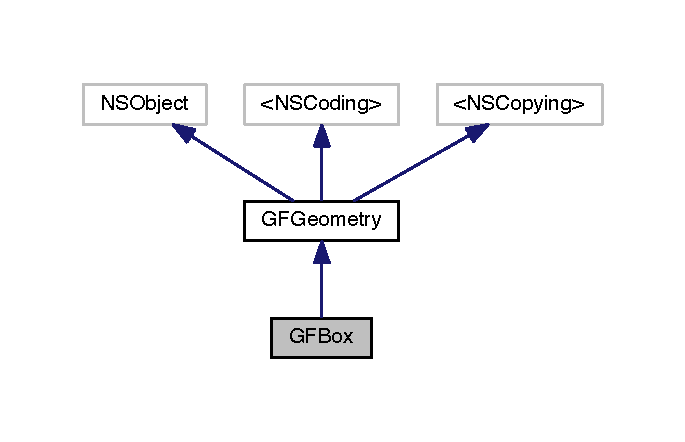
\includegraphics[width=350pt]{interface_g_f_box__inherit__graph}
\end{center}
\end{figure}


Collaboration diagram for G\+F\+Box\+:\nopagebreak
\begin{figure}[H]
\begin{center}
\leavevmode
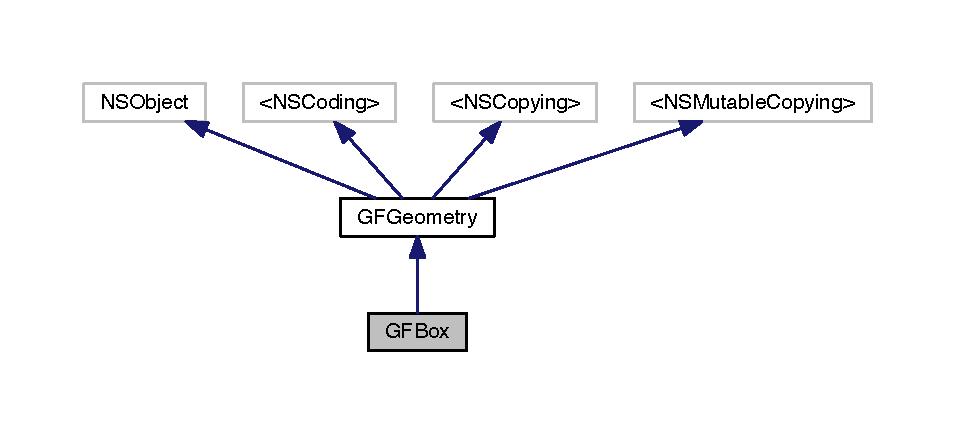
\includegraphics[width=350pt]{interface_g_f_box__coll__graph}
\end{center}
\end{figure}
\subsection*{Instance Methods}
\begin{DoxyCompactItemize}
\item 
(instancetype) -\/ \hyperlink{interface_g_f_box_a87bf50c9385711b4fed6c5ec9552397e}{init\+With\+Min\+Corner\+:max\+Corner\+:}
\item 
(instancetype) -\/ \hyperlink{interface_g_f_box_ab1c15e82e6b01e415e5fad629ac34ca4}{init\+With\+W\+K\+T\+:}
\item 
(instancetype) -\/ \hyperlink{interface_g_f_box_aaf52166ac0f936a32a04346ab91f2033}{init\+With\+W\+K\+T\+:error\+:}
\item 
(instancetype) -\/ \hyperlink{interface_g_f_box_a4865745ca621d9ee91186301d1bee3b3}{init\+With\+Geo\+J\+S\+O\+N\+Geometry\+:}
\item 
(instancetype) -\/ \hyperlink{interface_g_f_box_ad7feeb72217dbd9a8d89336f15455cb7}{init\+With\+Geo\+J\+S\+O\+N\+Geometry\+:error\+:}
\item 
(\hyperlink{interface_g_f_point}{G\+F\+Point} $\ast$) -\/ \hyperlink{interface_g_f_box_a102f7c53d4871e5431e813a2cb43eccd}{min\+Corner}
\item 
(\hyperlink{interface_g_f_point}{G\+F\+Point} $\ast$) -\/ \hyperlink{interface_g_f_box_ac2926a7b4f4f826f769a6f59aecd6f64}{max\+Corner}
\end{DoxyCompactItemize}
\subsection*{Additional Inherited Members}


\subsection{Detailed Description}
\hyperlink{interface_g_f_box}{G\+F\+Box} represents a simple box geometry. 

The \hyperlink{interface_g_f_box}{G\+F\+Box} class represents a simple box geometry and is represented as min and max corner G\+F\+Points.

\begin{DoxyAuthor}{Author}
Tony Stone 
\end{DoxyAuthor}
\begin{DoxyDate}{Date}
6/4/15 
\end{DoxyDate}


\subsection{Method Documentation}
\hypertarget{interface_g_f_box_a87bf50c9385711b4fed6c5ec9552397e}{}\index{G\+F\+Box@{G\+F\+Box}!init\+With\+Min\+Corner\+:max\+Corner\+:@{init\+With\+Min\+Corner\+:max\+Corner\+:}}
\index{init\+With\+Min\+Corner\+:max\+Corner\+:@{init\+With\+Min\+Corner\+:max\+Corner\+:}!G\+F\+Box@{G\+F\+Box}}
\subsubsection[{init\+With\+Min\+Corner\+:max\+Corner\+:(\+G\+F\+Point $\ast$min\+Corner,[max\+Corner] G\+F\+Point $\ast$max\+Corner)}]{\setlength{\rightskip}{0pt plus 5cm}-\/ (instancetype) init\+With\+Min\+Corner\+: 
\begin{DoxyParamCaption}
\item[{({\bf G\+F\+Point} $\ast$)}]{min\+Corner}
\item[{maxCorner:({\bf G\+F\+Point} $\ast$)}]{max\+Corner}
\end{DoxyParamCaption}
}\label{interface_g_f_box_a87bf50c9385711b4fed6c5ec9552397e}
Initialize this \hyperlink{interface_g_f_box}{G\+F\+Box} with 2 points representing the min and max point in the box. \hypertarget{interface_g_f_box_ab1c15e82e6b01e415e5fad629ac34ca4}{}\index{G\+F\+Box@{G\+F\+Box}!init\+With\+W\+K\+T\+:@{init\+With\+W\+K\+T\+:}}
\index{init\+With\+W\+K\+T\+:@{init\+With\+W\+K\+T\+:}!G\+F\+Box@{G\+F\+Box}}
\subsubsection[{init\+With\+W\+K\+T\+:(\+N\+S\+String $\ast$wkt)}]{\setlength{\rightskip}{0pt plus 5cm}-\/ (instancetype) init\+With\+W\+K\+T\+: 
\begin{DoxyParamCaption}
\item[{(N\+S\+String $\ast$)}]{wkt}
\end{DoxyParamCaption}
}\label{interface_g_f_box_ab1c15e82e6b01e415e5fad629ac34ca4}
Initialize this geometry with the given W\+K\+T (Well-\/\+Known-\/\+Text) string.

\begin{DoxyNote}{Note}


W\+K\+T does not support boxes. However, to be generic Geo\+Features supports reading and writing from and to boxes. Boxes are outputted as a standard P\+O\+L\+Y\+G\+O\+N W\+K\+T.

Geo\+Features can read boxes from a standard P\+O\+L\+Y\+G\+O\+N, from a P\+O\+L\+Y\+G\+O\+N with 2 points or from a B\+O\+X

The W\+K\+T output will always be a P\+O\+L\+Y\+G\+O\+N 
\end{DoxyNote}


Example\+: 
\begin{DoxyCode}
\{

  NSString * wkt = \textcolor{stringliteral}{@"POLYGON((0 0,0 90,90 90,90 0,0 0))"};

  \hyperlink{interface_g_f_box}{GFBox} * box = [[\hyperlink{interface_g_f_box}{GFBox} alloc] initWithWKT: wkt]];

\}
\end{DoxyCode}
 \hypertarget{interface_g_f_box_aaf52166ac0f936a32a04346ab91f2033}{}\index{G\+F\+Box@{G\+F\+Box}!init\+With\+W\+K\+T\+:error\+:@{init\+With\+W\+K\+T\+:error\+:}}
\index{init\+With\+W\+K\+T\+:error\+:@{init\+With\+W\+K\+T\+:error\+:}!G\+F\+Box@{G\+F\+Box}}
\subsubsection[{init\+With\+W\+K\+T\+:error\+:(\+N\+S\+String $\ast$wkt,[error] N\+S\+Error $\ast$\+\_\+\+\_\+autoreleasing $\ast$\+\_\+\+Nullable error)}]{\setlength{\rightskip}{0pt plus 5cm}-\/ (instancetype) {\bf init\+With\+W\+K\+T\+:} 
\begin{DoxyParamCaption}
\item[{(N\+S\+String $\ast$)}]{wkt}
\item[{error:(N\+S\+Error $\ast$\+\_\+\+\_\+autoreleasing $\ast$\+\_\+\+Nullable)}]{error}
\end{DoxyParamCaption}
}\label{interface_g_f_box_aaf52166ac0f936a32a04346ab91f2033}
Initialize this geometry with the given W\+K\+T (Well-\/\+Known-\/\+Text) string.

\begin{DoxyNote}{Note}


W\+K\+T does not support boxes. However, to be generic Geo\+Features supports reading and writing from and to boxes. Boxes are outputted as a standard P\+O\+L\+Y\+G\+O\+N W\+K\+T.

Geo\+Features can read boxes from a standard P\+O\+L\+Y\+G\+O\+N, from a P\+O\+L\+Y\+G\+O\+N with 2 points or from a B\+O\+X

The W\+K\+T output will always be a P\+O\+L\+Y\+G\+O\+N 
\end{DoxyNote}


Example\+: 
\begin{DoxyCode}
\{

  NSString * wkt = \textcolor{stringliteral}{@"POLYGON((0 0,0 90,90 90,90 0,0 0))"};

  NSError * error = nil;

  \hyperlink{interface_g_f_box}{GFBox} * box = [[\hyperlink{interface_g_f_box}{GFBox} alloc] initWithWKT: wkt error: &error]];

\}
\end{DoxyCode}
 \hypertarget{interface_g_f_box_a4865745ca621d9ee91186301d1bee3b3}{}\index{G\+F\+Box@{G\+F\+Box}!init\+With\+Geo\+J\+S\+O\+N\+Geometry\+:@{init\+With\+Geo\+J\+S\+O\+N\+Geometry\+:}}
\index{init\+With\+Geo\+J\+S\+O\+N\+Geometry\+:@{init\+With\+Geo\+J\+S\+O\+N\+Geometry\+:}!G\+F\+Box@{G\+F\+Box}}
\subsubsection[{init\+With\+Geo\+J\+S\+O\+N\+Geometry\+:(\+N\+S\+Dictionary $\ast$json\+Dictionary)}]{\setlength{\rightskip}{0pt plus 5cm}-\/ (instancetype) init\+With\+Geo\+J\+S\+O\+N\+Geometry\+: 
\begin{DoxyParamCaption}
\item[{(N\+S\+Dictionary $\ast$)}]{json\+Dictionary}
\end{DoxyParamCaption}
}\label{interface_g_f_box_a4865745ca621d9ee91186301d1bee3b3}
Initialize this geometry with the given json\+Dictionary.

\begin{DoxyNote}{Note}


You must pass the geometry portion of the Geo\+J\+S\+O\+N structure and not the entire Geo\+J\+S\+O\+N object.

Example\+:


\begin{DoxyCode}
\{
      \textcolor{stringliteral}{"type"}: \textcolor{stringliteral}{"Feature"},

      \textcolor{stringliteral}{"geometry"}:  \{
          \textcolor{stringliteral}{"type"}: \textcolor{stringliteral}{"Box"},
          \textcolor{stringliteral}{"coordinates"}: [[100.0, 0.0], [101.0, 1.0]]
      \}
 \}
\end{DoxyCode}


In the above example only the dictionary below that represents the geometry portion is passed.


\begin{DoxyCode}
\{
    \textcolor{stringliteral}{"type"}: \textcolor{stringliteral}{"Box"},
    \textcolor{stringliteral}{"coordinates"}: [[100.0, 0.0], [101.0, 1.0]]
\}
\end{DoxyCode}
 
\end{DoxyNote}
\hypertarget{interface_g_f_box_ad7feeb72217dbd9a8d89336f15455cb7}{}\index{G\+F\+Box@{G\+F\+Box}!init\+With\+Geo\+J\+S\+O\+N\+Geometry\+:error\+:@{init\+With\+Geo\+J\+S\+O\+N\+Geometry\+:error\+:}}
\index{init\+With\+Geo\+J\+S\+O\+N\+Geometry\+:error\+:@{init\+With\+Geo\+J\+S\+O\+N\+Geometry\+:error\+:}!G\+F\+Box@{G\+F\+Box}}
\subsubsection[{init\+With\+Geo\+J\+S\+O\+N\+Geometry\+:error\+:(\+N\+S\+Dictionary $\ast$json\+Dictionary,[error] N\+S\+Error $\ast$\+\_\+\+\_\+autoreleasing $\ast$error)}]{\setlength{\rightskip}{0pt plus 5cm}-\/ (instancetype) {\bf init\+With\+Geo\+J\+S\+O\+N\+Geometry\+:} 
\begin{DoxyParamCaption}
\item[{(N\+S\+Dictionary $\ast$)}]{json\+Dictionary}
\item[{error:(N\+S\+Error $\ast$\+\_\+\+\_\+autoreleasing $\ast$)}]{error}
\end{DoxyParamCaption}
}\label{interface_g_f_box_ad7feeb72217dbd9a8d89336f15455cb7}
Initialize this geometry with the given json\+Dictionary.

\begin{DoxyNote}{Note}


You must pass the geometry portion of the Geo\+J\+S\+O\+N structure and not the entire Geo\+J\+S\+O\+N object.

Example\+:


\begin{DoxyCode}
\{
      \textcolor{stringliteral}{"type"}: \textcolor{stringliteral}{"Feature"},

      \textcolor{stringliteral}{"geometry"}:  \{
          \textcolor{stringliteral}{"type"}: \textcolor{stringliteral}{"Box"},
          \textcolor{stringliteral}{"coordinates"}: [[100.0, 0.0], [101.0, 1.0]]
      \}
 \}
\end{DoxyCode}


In the above example only the dictionary below that represents the geometry portion is passed.


\begin{DoxyCode}
\{
    \textcolor{stringliteral}{"type"}: \textcolor{stringliteral}{"Box"},
    \textcolor{stringliteral}{"coordinates"}: [[100.0, 0.0], [101.0, 1.0]]
\}
\end{DoxyCode}
 
\end{DoxyNote}
\hypertarget{interface_g_f_box_a102f7c53d4871e5431e813a2cb43eccd}{}\index{G\+F\+Box@{G\+F\+Box}!min\+Corner@{min\+Corner}}
\index{min\+Corner@{min\+Corner}!G\+F\+Box@{G\+F\+Box}}
\subsubsection[{min\+Corner()}]{\setlength{\rightskip}{0pt plus 5cm}-\/ ({\bf G\+F\+Point} $\ast$) min\+Corner 
\begin{DoxyParamCaption}
{}
\end{DoxyParamCaption}
}\label{interface_g_f_box_a102f7c53d4871e5431e813a2cb43eccd}
\begin{DoxyReturn}{Returns}
The min\+Corner \hyperlink{interface_g_f_point}{G\+F\+Point} from this \hyperlink{interface_g_f_box}{G\+F\+Box} 
\end{DoxyReturn}
\hypertarget{interface_g_f_box_ac2926a7b4f4f826f769a6f59aecd6f64}{}\index{G\+F\+Box@{G\+F\+Box}!max\+Corner@{max\+Corner}}
\index{max\+Corner@{max\+Corner}!G\+F\+Box@{G\+F\+Box}}
\subsubsection[{max\+Corner()}]{\setlength{\rightskip}{0pt plus 5cm}-\/ ({\bf G\+F\+Point} $\ast$) max\+Corner 
\begin{DoxyParamCaption}
{}
\end{DoxyParamCaption}
}\label{interface_g_f_box_ac2926a7b4f4f826f769a6f59aecd6f64}
\begin{DoxyReturn}{Returns}
The max\+Corner \hyperlink{interface_g_f_point}{G\+F\+Point} from this \hyperlink{interface_g_f_box}{G\+F\+Box} 
\end{DoxyReturn}


The documentation for this class was generated from the following file\+:\begin{DoxyCompactItemize}
\item 
Geo\+Features/G\+F\+Box.\+h\end{DoxyCompactItemize}

\hypertarget{interface_g_f_geometry}{}\section{G\+F\+Geometry Class Reference}
\label{interface_g_f_geometry}\index{G\+F\+Geometry@{G\+F\+Geometry}}


An abstract class that represents a geometric shape.  




{\ttfamily \#import $<$Geo\+Features/\+G\+F\+Geometry.\+h$>$}



Inheritance diagram for G\+F\+Geometry\+:\nopagebreak
\begin{figure}[H]
\begin{center}
\leavevmode
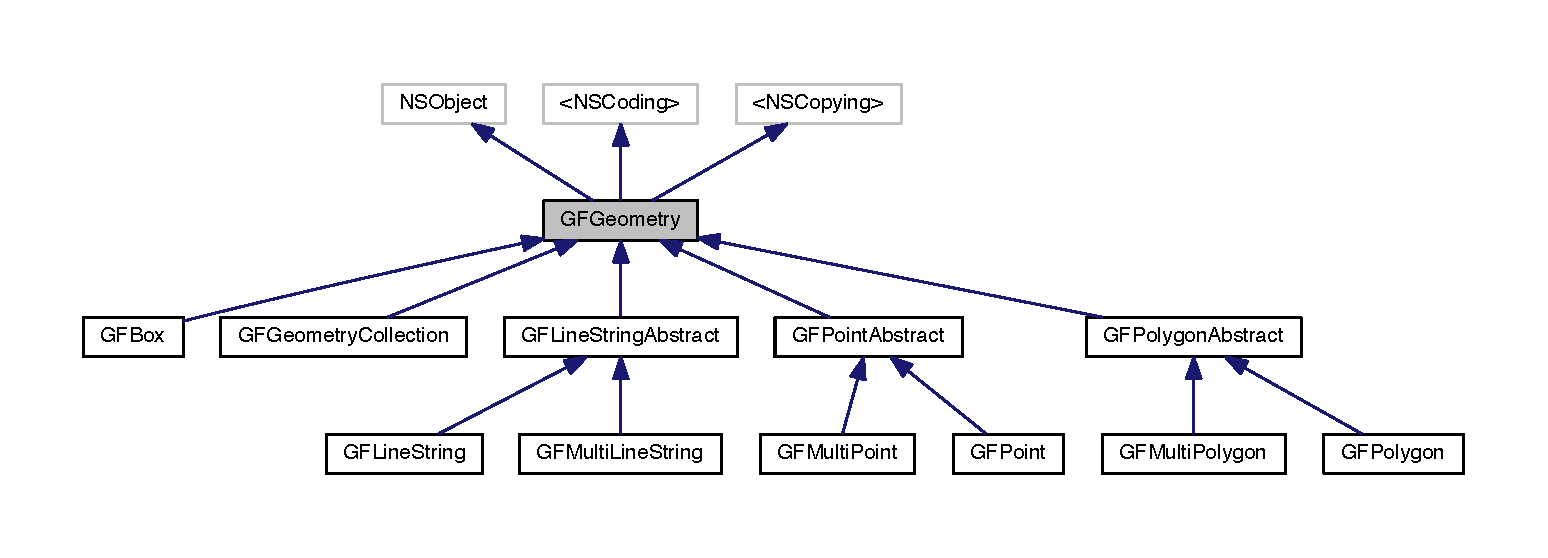
\includegraphics[width=350pt]{interface_g_f_geometry__inherit__graph}
\end{center}
\end{figure}


Collaboration diagram for G\+F\+Geometry\+:\nopagebreak
\begin{figure}[H]
\begin{center}
\leavevmode
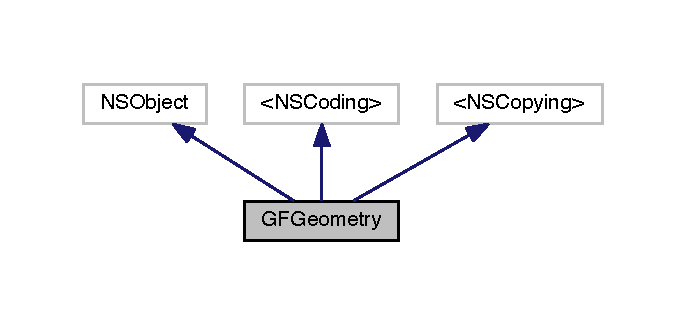
\includegraphics[width=350pt]{interface_g_f_geometry__coll__graph}
\end{center}
\end{figure}
\subsection*{Instance Methods}
\begin{DoxyCompactItemize}
\item 
(B\+O\+O\+L) -\/ \hyperlink{interface_g_f_geometry_a3a63de5905eae52356c6afd7313e4828}{is\+Valid}
\item 
(double) -\/ \hyperlink{interface_g_f_geometry_a0028dc3b2c2315a24d803dfa4cf2250e}{area}
\item 
(double) -\/ \hyperlink{interface_g_f_geometry_ab68dd3c418a3f06c6593d02dfebe2585}{length}
\item 
(double) -\/ \hyperlink{interface_g_f_geometry_a31593eea12da7a9ed46b2dd4e6ca511e}{perimeter}
\item 
(\hyperlink{interface_g_f_point}{G\+F\+Point} $\ast$) -\/ \hyperlink{interface_g_f_geometry_af53b7bf19dfea6827eed19a7979c7dca}{centroid}
\item 
(\hyperlink{interface_g_f_point}{G\+F\+Point} $\ast$) -\/ \hyperlink{interface_g_f_geometry_a16f03e92b3636e574d5f8659e822de69}{centroid\+:}
\item 
(\hyperlink{interface_g_f_box}{G\+F\+Box} $\ast$) -\/ \hyperlink{interface_g_f_geometry_a808ba7daf6d4c3d742668ad3fe5d0f0e}{bounding\+Box}
\item 
(B\+O\+O\+L) -\/ \hyperlink{interface_g_f_geometry_a832350c76f4a42a39889c9138108edd2}{within\+:}
\item 
(B\+O\+O\+L) -\/ \hyperlink{interface_g_f_geometry_a3735ea20bc337cff79944bbe08f3bdf0}{intersects}
\item 
(B\+O\+O\+L) -\/ \hyperlink{interface_g_f_geometry_a86d1a80435c6b838dfb8b1a22a17a0b8}{intersects\+:}
\item 
(\hyperlink{interface_g_f_geometry}{G\+F\+Geometry} $\ast$) -\/ \hyperlink{interface_g_f_geometry_ac93053aeabad1f97466b1ec31292ed11}{intersection\+:}
\item 
(\hyperlink{interface_g_f_geometry}{G\+F\+Geometry} $\ast$) -\/ \hyperlink{interface_g_f_geometry_a6faa39e502da86516c58b5ce65847924}{intersection\+:error\+:}
\item 
(\hyperlink{interface_g_f_geometry}{G\+F\+Geometry} $\ast$) -\/ \hyperlink{interface_g_f_geometry_acb76057cb6cdee9255ecba8447045cc6}{difference\+:}
\item 
(\hyperlink{interface_g_f_geometry}{G\+F\+Geometry} $\ast$) -\/ \hyperlink{interface_g_f_geometry_a30eb0242f8e9f9e3e1d542af03e4144b}{difference\+:error\+:}
\item 
(\hyperlink{interface_g_f_geometry}{G\+F\+Geometry} $\ast$) -\/ \hyperlink{interface_g_f_geometry_a58c32fcf4a3932281498d1a1b25fb46b}{union\+\_\+\+:}
\item 
(\hyperlink{interface_g_f_geometry}{G\+F\+Geometry} $\ast$) -\/ \hyperlink{interface_g_f_geometry_ac3fa56a053de364baf4b9c496b0b93a4}{union\+\_\+\+:error\+:}
\item 
(N\+S\+Dictionary $\ast$) -\/ \hyperlink{interface_g_f_geometry_a89a1dd53c1d9a51fd5b933fde28be5b7}{to\+Geo\+J\+S\+O\+N\+Geometry}
\item 
(N\+S\+Array $\ast$) -\/ \hyperlink{interface_g_f_geometry_a69a56e7786e1de09034c546ade1c7262}{mk\+Map\+Overlays}
\item 
(N\+S\+String $\ast$) -\/ \hyperlink{interface_g_f_geometry_a9d257cce05d031211e2cece24b5530e4}{to\+W\+K\+T\+String}
\end{DoxyCompactItemize}
\subsection*{Class Methods}
\begin{DoxyCompactItemize}
\item 
(instancetype) + \hyperlink{interface_g_f_geometry_a5b730dcea33fc8b2c156199400e3014e}{geometry\+With\+Geo\+J\+S\+O\+N\+Geometry\+:}
\item 
(instancetype) + \hyperlink{interface_g_f_geometry_ac665565535c19e73e6b7a696e8109586}{geometry\+With\+Geo\+J\+S\+O\+N\+Geometry\+:error\+:}
\item 
(instancetype) + \hyperlink{interface_g_f_geometry_a32a49e08fdbc2998735c26ddbfa88741}{geometry\+With\+W\+K\+T\+:}
\item 
(instancetype) + \hyperlink{interface_g_f_geometry_a04922dcfc9db4543970774b0457d487b}{geometry\+With\+W\+K\+T\+:error\+:}
\end{DoxyCompactItemize}


\subsection{Detailed Description}
An abstract class that represents a geometric shape. 

\hyperlink{interface_g_f_geometry}{G\+F\+Geometry} is the abstract base class for all geometry subclasses. It is also the central factory object for creation of geometries.

\begin{DoxyWarning}{Warning}
Do not instantiate this abstract class.
\end{DoxyWarning}
\begin{DoxyAuthor}{Author}
Tony Stone 
\end{DoxyAuthor}
\begin{DoxyDate}{Date}
6/14/15 
\end{DoxyDate}


\subsection{Method Documentation}
\hypertarget{interface_g_f_geometry_a3a63de5905eae52356c6afd7313e4828}{}\index{G\+F\+Geometry@{G\+F\+Geometry}!is\+Valid@{is\+Valid}}
\index{is\+Valid@{is\+Valid}!G\+F\+Geometry@{G\+F\+Geometry}}
\subsubsection[{is\+Valid()}]{\setlength{\rightskip}{0pt plus 5cm}-\/ (B\+O\+O\+L) is\+Valid 
\begin{DoxyParamCaption}
{}
\end{DoxyParamCaption}
}\label{interface_g_f_geometry_a3a63de5905eae52356c6afd7313e4828}
Checks if a geometry is valid. \hypertarget{interface_g_f_geometry_a0028dc3b2c2315a24d803dfa4cf2250e}{}\index{G\+F\+Geometry@{G\+F\+Geometry}!area@{area}}
\index{area@{area}!G\+F\+Geometry@{G\+F\+Geometry}}
\subsubsection[{area()}]{\setlength{\rightskip}{0pt plus 5cm}-\/ (double) area 
\begin{DoxyParamCaption}
{}
\end{DoxyParamCaption}
}\label{interface_g_f_geometry_a0028dc3b2c2315a24d803dfa4cf2250e}
The area algorithm calculates the surface area of all geometries having a surface, namely box, polygon, ring, multipolygon. The units are the square of the units used for the points defining the surface. If subject geometry is defined in meters, then area is calculated in square meters

\begin{DoxyReturn}{Returns}
The area of the geometry. 
\end{DoxyReturn}
\hypertarget{interface_g_f_geometry_ab68dd3c418a3f06c6593d02dfebe2585}{}\index{G\+F\+Geometry@{G\+F\+Geometry}!length@{length}}
\index{length@{length}!G\+F\+Geometry@{G\+F\+Geometry}}
\subsubsection[{length()}]{\setlength{\rightskip}{0pt plus 5cm}-\/ (double) length 
\begin{DoxyParamCaption}
{}
\end{DoxyParamCaption}
}\label{interface_g_f_geometry_ab68dd3c418a3f06c6593d02dfebe2585}
The length method calculates the length (the sum of distances between consecutive points) of a geometry.

\begin{DoxyNote}{Note}


point types (e.\+g. \hyperlink{interface_g_f_point}{G\+F\+Point}) Return zero

linear types (e.\+g. \hyperlink{interface_g_f_line_string}{G\+F\+Line\+String}) Return the length

areal (e.\+g. \hyperlink{interface_g_f_polygon}{G\+F\+Polygon}) Return zero




\end{DoxyNote}
\begin{DoxyReturn}{Returns}
The length of linear \hyperlink{interface_g_f_geometry}{G\+F\+Geometry} types (e.\+g. \hyperlink{interface_g_f_line_string}{G\+F\+Line\+String}). 
\end{DoxyReturn}
\hypertarget{interface_g_f_geometry_a31593eea12da7a9ed46b2dd4e6ca511e}{}\index{G\+F\+Geometry@{G\+F\+Geometry}!perimeter@{perimeter}}
\index{perimeter@{perimeter}!G\+F\+Geometry@{G\+F\+Geometry}}
\subsubsection[{perimeter()}]{\setlength{\rightskip}{0pt plus 5cm}-\/ (double) perimeter 
\begin{DoxyParamCaption}
{}
\end{DoxyParamCaption}
}\label{interface_g_f_geometry_a31593eea12da7a9ed46b2dd4e6ca511e}
Calculates the perimeter of a geometry

\begin{DoxyNote}{Note}


point types (e.\+g. \hyperlink{interface_g_f_point}{G\+F\+Point}) Returns zero

linear types (e.\+g. \hyperlink{interface_g_f_line_string}{G\+F\+Line\+String}) Returns zero

areal (e.\+g. \hyperlink{interface_g_f_polygon}{G\+F\+Polygon}) Returns the perimeter


\end{DoxyNote}


\begin{DoxyReturn}{Returns}
The perimeter of areal \hyperlink{interface_g_f_geometry}{G\+F\+Geometry} types (e.\+g. \hyperlink{interface_g_f_polygon}{G\+F\+Polygon}). 
\end{DoxyReturn}
\hypertarget{interface_g_f_geometry_af53b7bf19dfea6827eed19a7979c7dca}{}\index{G\+F\+Geometry@{G\+F\+Geometry}!centroid@{centroid}}
\index{centroid@{centroid}!G\+F\+Geometry@{G\+F\+Geometry}}
\subsubsection[{centroid()}]{\setlength{\rightskip}{0pt plus 5cm}-\/ ({\bf G\+F\+Point} $\ast$) centroid 
\begin{DoxyParamCaption}
{}
\end{DoxyParamCaption}
}\label{interface_g_f_geometry_af53b7bf19dfea6827eed19a7979c7dca}
The centroid method calculates the geometric center (or\+: center of mass) of a geometry.

\begin{DoxyReturn}{Returns}
The calculated centroid as a \hyperlink{interface_g_f_point}{G\+F\+Point}. 
\end{DoxyReturn}
\hypertarget{interface_g_f_geometry_a16f03e92b3636e574d5f8659e822de69}{}\index{G\+F\+Geometry@{G\+F\+Geometry}!centroid\+:@{centroid\+:}}
\index{centroid\+:@{centroid\+:}!G\+F\+Geometry@{G\+F\+Geometry}}
\subsubsection[{centroid\+:(\+N\+S\+Error $\ast$\+\_\+\+\_\+autoreleasing $\ast$error)}]{\setlength{\rightskip}{0pt plus 5cm}-\/ ({\bf G\+F\+Point} $\ast$) centroid\+: 
\begin{DoxyParamCaption}
\item[{(N\+S\+Error $\ast$\+\_\+\+\_\+autoreleasing $\ast$)}]{error}
\end{DoxyParamCaption}
}\label{interface_g_f_geometry_a16f03e92b3636e574d5f8659e822de69}
The centroid method calculates the geometric center (or\+: center of mass) of a geometry.

\begin{DoxyReturn}{Returns}
The calculated centroid as a \hyperlink{interface_g_f_point}{G\+F\+Point}. 
\end{DoxyReturn}
\hypertarget{interface_g_f_geometry_a808ba7daf6d4c3d742668ad3fe5d0f0e}{}\index{G\+F\+Geometry@{G\+F\+Geometry}!bounding\+Box@{bounding\+Box}}
\index{bounding\+Box@{bounding\+Box}!G\+F\+Geometry@{G\+F\+Geometry}}
\subsubsection[{bounding\+Box()}]{\setlength{\rightskip}{0pt plus 5cm}-\/ ({\bf G\+F\+Box} $\ast$) bounding\+Box 
\begin{DoxyParamCaption}
{}
\end{DoxyParamCaption}
}\label{interface_g_f_geometry_a808ba7daf6d4c3d742668ad3fe5d0f0e}
The bounding\+Box method calculates the bounding\+Box (also known as axis aligned bounding box, aabb, or minimum bounding rectangle, mbr) of a geometry.

\begin{DoxyReturn}{Returns}
The bounding box as a \hyperlink{interface_g_f_box}{G\+F\+Box}. 
\end{DoxyReturn}
\hypertarget{interface_g_f_geometry_a832350c76f4a42a39889c9138108edd2}{}\index{G\+F\+Geometry@{G\+F\+Geometry}!within\+:@{within\+:}}
\index{within\+:@{within\+:}!G\+F\+Geometry@{G\+F\+Geometry}}
\subsubsection[{within\+:(\+G\+F\+Geometry $\ast$other)}]{\setlength{\rightskip}{0pt plus 5cm}-\/ (B\+O\+O\+L) within\+: 
\begin{DoxyParamCaption}
\item[{({\bf G\+F\+Geometry} $\ast$)}]{other}
\end{DoxyParamCaption}
}\label{interface_g_f_geometry_a832350c76f4a42a39889c9138108edd2}
Checks if the geometry is completely inside the other geometry.

\begin{DoxyReturn}{Returns}
True if self is within the other \hyperlink{interface_g_f_geometry}{G\+F\+Geometry} instance. False otherwise. 
\end{DoxyReturn}
\hypertarget{interface_g_f_geometry_a3735ea20bc337cff79944bbe08f3bdf0}{}\index{G\+F\+Geometry@{G\+F\+Geometry}!intersects@{intersects}}
\index{intersects@{intersects}!G\+F\+Geometry@{G\+F\+Geometry}}
\subsubsection[{intersects()}]{\setlength{\rightskip}{0pt plus 5cm}-\/ (B\+O\+O\+L) intersects 
\begin{DoxyParamCaption}
{}
\end{DoxyParamCaption}
}\label{interface_g_f_geometry_a3735ea20bc337cff79944bbe08f3bdf0}
Checks if self has at least one intersection.

\begin{DoxyReturn}{Returns}
true if self has at least one intersection. 
\end{DoxyReturn}
\hypertarget{interface_g_f_geometry_a86d1a80435c6b838dfb8b1a22a17a0b8}{}\index{G\+F\+Geometry@{G\+F\+Geometry}!intersects\+:@{intersects\+:}}
\index{intersects\+:@{intersects\+:}!G\+F\+Geometry@{G\+F\+Geometry}}
\subsubsection[{intersects\+:(\+G\+F\+Geometry $\ast$other)}]{\setlength{\rightskip}{0pt plus 5cm}-\/ (B\+O\+O\+L) intersects\+: 
\begin{DoxyParamCaption}
\item[{({\bf G\+F\+Geometry} $\ast$)}]{other}
\end{DoxyParamCaption}
}\label{interface_g_f_geometry_a86d1a80435c6b838dfb8b1a22a17a0b8}
Checks if self has at least one intersection with the other geometry.

\begin{DoxyReturn}{Returns}
true if self has at least one intersection with the other geometry. 
\end{DoxyReturn}
\hypertarget{interface_g_f_geometry_ac93053aeabad1f97466b1ec31292ed11}{}\index{G\+F\+Geometry@{G\+F\+Geometry}!intersection\+:@{intersection\+:}}
\index{intersection\+:@{intersection\+:}!G\+F\+Geometry@{G\+F\+Geometry}}
\subsubsection[{intersection\+:(\+G\+F\+Geometry $\ast$other)}]{\setlength{\rightskip}{0pt plus 5cm}-\/ ({\bf G\+F\+Geometry} $\ast$) intersection\+: 
\begin{DoxyParamCaption}
\item[{({\bf G\+F\+Geometry} $\ast$)}]{other}
\end{DoxyParamCaption}
}\label{interface_g_f_geometry_ac93053aeabad1f97466b1ec31292ed11}
Calculates the point set intersection of this geometry with other.

\begin{DoxyReturn}{Returns}
A geometry object that represents the point set intersection of this geometric object with other.
\end{DoxyReturn}

\begin{DoxyExceptions}{Exceptions}
{\em N\+S\+Invalid\+Argument\+Exception} & If the an intersection between self and other are not supported. \\
\hline
\end{DoxyExceptions}
\hypertarget{interface_g_f_geometry_a6faa39e502da86516c58b5ce65847924}{}\index{G\+F\+Geometry@{G\+F\+Geometry}!intersection\+:error\+:@{intersection\+:error\+:}}
\index{intersection\+:error\+:@{intersection\+:error\+:}!G\+F\+Geometry@{G\+F\+Geometry}}
\subsubsection[{intersection\+:error\+:(\+G\+F\+Geometry $\ast$other,[error] N\+S\+Error $\ast$\+\_\+\+\_\+autoreleasing $\ast$error)}]{\setlength{\rightskip}{0pt plus 5cm}-\/ ({\bf G\+F\+Geometry} $\ast$) {\bf intersection\+:} 
\begin{DoxyParamCaption}
\item[{({\bf G\+F\+Geometry} $\ast$)}]{other}
\item[{error:(N\+S\+Error $\ast$\+\_\+\+\_\+autoreleasing $\ast$)}]{error}
\end{DoxyParamCaption}
}\label{interface_g_f_geometry_a6faa39e502da86516c58b5ce65847924}
Calculates the point set intersection of this geometry with other.

\begin{DoxyReturn}{Returns}
A geometry object that represents the point set intersection of this geometric object with other. 
\end{DoxyReturn}
\hypertarget{interface_g_f_geometry_acb76057cb6cdee9255ecba8447045cc6}{}\index{G\+F\+Geometry@{G\+F\+Geometry}!difference\+:@{difference\+:}}
\index{difference\+:@{difference\+:}!G\+F\+Geometry@{G\+F\+Geometry}}
\subsubsection[{difference\+:(\+G\+F\+Geometry $\ast$other)}]{\setlength{\rightskip}{0pt plus 5cm}-\/ ({\bf G\+F\+Geometry} $\ast$) difference\+: 
\begin{DoxyParamCaption}
\item[{({\bf G\+F\+Geometry} $\ast$)}]{other}
\end{DoxyParamCaption}
}\label{interface_g_f_geometry_acb76057cb6cdee9255ecba8447045cc6}
Calculate the difference of two geometries.

\begin{DoxyReturn}{Returns}
A new \hyperlink{interface_g_f_geometry}{G\+F\+Geometry} instance that represents the difference of self and other.
\end{DoxyReturn}

\begin{DoxyExceptions}{Exceptions}
{\em N\+S\+Invalid\+Argument\+Exception} & If the difference between self and other are not supported. \\
\hline
\end{DoxyExceptions}
\hypertarget{interface_g_f_geometry_a30eb0242f8e9f9e3e1d542af03e4144b}{}\index{G\+F\+Geometry@{G\+F\+Geometry}!difference\+:error\+:@{difference\+:error\+:}}
\index{difference\+:error\+:@{difference\+:error\+:}!G\+F\+Geometry@{G\+F\+Geometry}}
\subsubsection[{difference\+:error\+:(\+G\+F\+Geometry $\ast$other,[error] N\+S\+Error $\ast$\+\_\+\+\_\+autoreleasing $\ast$error)}]{\setlength{\rightskip}{0pt plus 5cm}-\/ ({\bf G\+F\+Geometry} $\ast$) {\bf difference\+:} 
\begin{DoxyParamCaption}
\item[{({\bf G\+F\+Geometry} $\ast$)}]{other}
\item[{error:(N\+S\+Error $\ast$\+\_\+\+\_\+autoreleasing $\ast$)}]{error}
\end{DoxyParamCaption}
}\label{interface_g_f_geometry_a30eb0242f8e9f9e3e1d542af03e4144b}
Calculate the difference of two geometries.

\begin{DoxyReturn}{Returns}
A new \hyperlink{interface_g_f_geometry}{G\+F\+Geometry} instance that represents the difference of self and other. 
\end{DoxyReturn}
\hypertarget{interface_g_f_geometry_a58c32fcf4a3932281498d1a1b25fb46b}{}\index{G\+F\+Geometry@{G\+F\+Geometry}!union\+\_\+\+:@{union\+\_\+\+:}}
\index{union\+\_\+\+:@{union\+\_\+\+:}!G\+F\+Geometry@{G\+F\+Geometry}}
\subsubsection[{union\+\_\+\+:(\+G\+F\+Geometry $\ast$other)}]{\setlength{\rightskip}{0pt plus 5cm}-\/ ({\bf G\+F\+Geometry} $\ast$) union\+\_\+\+: 
\begin{DoxyParamCaption}
\item[{({\bf G\+F\+Geometry} $\ast$)}]{other}
\end{DoxyParamCaption}
}\label{interface_g_f_geometry_a58c32fcf4a3932281498d1a1b25fb46b}
Combines the other geometry with self. The union calculates the spatial set theoretic union of the two geometries.

\begin{DoxyReturn}{Returns}
A new \hyperlink{interface_g_f_geometry}{G\+F\+Geometry} instance that represents the union of the and other.
\end{DoxyReturn}

\begin{DoxyExceptions}{Exceptions}
{\em N\+S\+Invalid\+Argument\+Exception} & if the one of the geometries is invalid. You can test for an invalid geometry by calling is\+Valid. \\
\hline
\end{DoxyExceptions}
\hypertarget{interface_g_f_geometry_ac3fa56a053de364baf4b9c496b0b93a4}{}\index{G\+F\+Geometry@{G\+F\+Geometry}!union\+\_\+\+:error\+:@{union\+\_\+\+:error\+:}}
\index{union\+\_\+\+:error\+:@{union\+\_\+\+:error\+:}!G\+F\+Geometry@{G\+F\+Geometry}}
\subsubsection[{union\+\_\+\+:error\+:(\+G\+F\+Geometry $\ast$other,[error] N\+S\+Error $\ast$\+\_\+\+\_\+autoreleasing $\ast$error)}]{\setlength{\rightskip}{0pt plus 5cm}-\/ ({\bf G\+F\+Geometry} $\ast$) {\bf union\+\_\+\+:} 
\begin{DoxyParamCaption}
\item[{({\bf G\+F\+Geometry} $\ast$)}]{other}
\item[{error:(N\+S\+Error $\ast$\+\_\+\+\_\+autoreleasing $\ast$)}]{error}
\end{DoxyParamCaption}
}\label{interface_g_f_geometry_ac3fa56a053de364baf4b9c496b0b93a4}
Combines the other geometry with self. The union calculates the spatial set theoretic union of the two geometries.

\begin{DoxyReturn}{Returns}
A new \hyperlink{interface_g_f_geometry}{G\+F\+Geometry} instance that represents the union of self and other. 
\end{DoxyReturn}
\hypertarget{interface_g_f_geometry_a5b730dcea33fc8b2c156199400e3014e}{}\index{G\+F\+Geometry@{G\+F\+Geometry}!geometry\+With\+Geo\+J\+S\+O\+N\+Geometry\+:@{geometry\+With\+Geo\+J\+S\+O\+N\+Geometry\+:}}
\index{geometry\+With\+Geo\+J\+S\+O\+N\+Geometry\+:@{geometry\+With\+Geo\+J\+S\+O\+N\+Geometry\+:}!G\+F\+Geometry@{G\+F\+Geometry}}
\subsubsection[{geometry\+With\+Geo\+J\+S\+O\+N\+Geometry\+:(\+N\+S\+Dictionary $\ast$geo\+J\+S\+O\+N\+Geometry\+Dictionary)}]{\setlength{\rightskip}{0pt plus 5cm}+ (instancetype) geometry\+With\+Geo\+J\+S\+O\+N\+Geometry\+: 
\begin{DoxyParamCaption}
\item[{(N\+S\+Dictionary $\ast$)}]{geo\+J\+S\+O\+N\+Geometry\+Dictionary}
\end{DoxyParamCaption}
}\label{interface_g_f_geometry_a5b730dcea33fc8b2c156199400e3014e}
Creates a \hyperlink{interface_g_f_geometry}{G\+F\+Geometry} from the Geo\+J\+S\+O\+N dictionary supplied.

\begin{DoxyNote}{Note}
You must pass the geometry portion of the Geo\+J\+S\+O\+N structure and not the entire Geo\+J\+S\+O\+N object. 

Given the following Geo\+J\+S\+O\+N\+: 
\begin{DoxyCode}
\{
      \textcolor{stringliteral}{"type"}: \textcolor{stringliteral}{"Feature"},

      \textcolor{stringliteral}{"geometry"}:  \{
          \textcolor{stringliteral}{"type"}: \textcolor{stringliteral}{"Box"},
          \textcolor{stringliteral}{"coordinates"}: [[100.0, 0.0], [101.0, 1.0]]
      \}
 \}
\end{DoxyCode}


You would pass the geometry section below to the init method. 
\begin{DoxyCode}
\{
    \textcolor{stringliteral}{"type"}: \textcolor{stringliteral}{"Box"},
    \textcolor{stringliteral}{"coordinates"}: [[100.0, 0.0], [101.0, 1.0]]
\}
\end{DoxyCode}
 
\end{DoxyNote}


Example\+: 
\begin{DoxyCode}
\{
    NSString * jsonString = \textcolor{stringliteral}{@"\{ \(\backslash\)"}type\(\backslash\)\textcolor{stringliteral}{": \(\backslash\)"Polygon\(\backslash\)","}
                             \textcolor{stringliteral}{"    \(\backslash\)"coordinates\(\backslash\)": ["}
                             \textcolor{stringliteral}{"      [ [100.0, 0.0], [200.0, 0.0], [200.0, 100.0], [100.0, 1.0], [100.0,
       0.0] ],"}
                             \textcolor{stringliteral}{"      [ [100.2, 0.2], [100.8, 0.2], [100.8, 0.8], [100.2, 0.8], [100.2, 0.2]
       ]"}
                             \textcolor{stringliteral}{"      ]"}
                             \textcolor{stringliteral}{"   \}"}

    NSDictionary * geometryDictionary = [NSJSONSerialization JSONObjectWithData: [jsonString 
      dataUsingEncoding: NSUTF8StringEncoding] options: 0 error: nil];

    \hyperlink{interface_g_f_geometry}{GFGeometry} * geometry = [\hyperlink{interface_g_f_geometry}{GFGeometry} geometryWithGeoJSONGeometry: geometryDictionary
       ]

\}
\end{DoxyCode}



\begin{DoxyExceptions}{Exceptions}
{\em N\+S\+Exception} & This method will throw an exception if the geo json is invalid. \\
\hline
\end{DoxyExceptions}


Provided by category \hyperlink{category_g_f_geometry_07_geo_j_s_o_n_08_a5b730dcea33fc8b2c156199400e3014e}{G\+F\+Geometry(\+Geo\+J\+S\+O\+N)}.

\hypertarget{interface_g_f_geometry_ac665565535c19e73e6b7a696e8109586}{}\index{G\+F\+Geometry@{G\+F\+Geometry}!geometry\+With\+Geo\+J\+S\+O\+N\+Geometry\+:error\+:@{geometry\+With\+Geo\+J\+S\+O\+N\+Geometry\+:error\+:}}
\index{geometry\+With\+Geo\+J\+S\+O\+N\+Geometry\+:error\+:@{geometry\+With\+Geo\+J\+S\+O\+N\+Geometry\+:error\+:}!G\+F\+Geometry@{G\+F\+Geometry}}
\subsubsection[{geometry\+With\+Geo\+J\+S\+O\+N\+Geometry\+:error\+:(\+N\+S\+Dictionary $\ast$geo\+J\+S\+O\+N\+Geometry\+Dictionary,[error] N\+S\+Error $\ast$\+\_\+\+\_\+autoreleasing $\ast$error)}]{\setlength{\rightskip}{0pt plus 5cm}+ (instancetype) {\bf geometry\+With\+Geo\+J\+S\+O\+N\+Geometry\+:} 
\begin{DoxyParamCaption}
\item[{(N\+S\+Dictionary $\ast$)}]{geo\+J\+S\+O\+N\+Geometry\+Dictionary}
\item[{error:(N\+S\+Error $\ast$\+\_\+\+\_\+autoreleasing $\ast$)}]{error}
\end{DoxyParamCaption}
}\label{interface_g_f_geometry_ac665565535c19e73e6b7a696e8109586}
Creates a \hyperlink{interface_g_f_geometry}{G\+F\+Geometry} from the Geo\+J\+S\+O\+N dictionary supplied.

\begin{DoxyNote}{Note}
You must pass the geometry portion of the Geo\+J\+S\+O\+N structure and not the entire Geo\+J\+S\+O\+N object. 

Given the following Geo\+J\+S\+O\+N\+: 
\begin{DoxyCode}
\{
      \textcolor{stringliteral}{"type"}: \textcolor{stringliteral}{"Feature"},

      \textcolor{stringliteral}{"geometry"}:  \{
          \textcolor{stringliteral}{"type"}: \textcolor{stringliteral}{"Box"},
          \textcolor{stringliteral}{"coordinates"}: [[100.0, 0.0], [101.0, 1.0]]
      \}
 \}
\end{DoxyCode}


You would pass the geometry section below to the init method. 
\begin{DoxyCode}
\{
    \textcolor{stringliteral}{"type"}: \textcolor{stringliteral}{"Box"},
    \textcolor{stringliteral}{"coordinates"}: [[100.0, 0.0], [101.0, 1.0]]
\}
\end{DoxyCode}
 
\end{DoxyNote}


Example\+: 
\begin{DoxyCode}
\{
    NSString * jsonString = \textcolor{stringliteral}{@"\{ \(\backslash\)"}type\(\backslash\)\textcolor{stringliteral}{": \(\backslash\)"Polygon\(\backslash\)","}
                             \textcolor{stringliteral}{"    \(\backslash\)"coordinates\(\backslash\)": ["}
                             \textcolor{stringliteral}{"      [ [100.0, 0.0], [200.0, 0.0], [200.0, 100.0], [100.0, 1.0], [100.0,
       0.0] ],"}
                             \textcolor{stringliteral}{"      [ [100.2, 0.2], [100.8, 0.2], [100.8, 0.8], [100.2, 0.8], [100.2, 0.2]
       ]"}
                             \textcolor{stringliteral}{"      ]"}
                             \textcolor{stringliteral}{"   \}"}

    NSDictionary * geometryDictionary = [NSJSONSerialization JSONObjectWithData: [jsonString 
      dataUsingEncoding: NSUTF8StringEncoding] options: 0 error: nil];

    \hyperlink{interface_g_f_geometry}{GFGeometry} * geometry = [\hyperlink{interface_g_f_geometry}{GFGeometry} geometryWithGeoJSONGeometry: geometryDictionary
       ]

\}
\end{DoxyCode}



\begin{DoxyExceptions}{Exceptions}
{\em N\+S\+Exception} & This method will throw an exception if the geo json is invalid. \\
\hline
\end{DoxyExceptions}


Provided by category \hyperlink{category_g_f_geometry_07_geo_j_s_o_n_08_ac665565535c19e73e6b7a696e8109586}{G\+F\+Geometry(\+Geo\+J\+S\+O\+N)}.

\hypertarget{interface_g_f_geometry_a89a1dd53c1d9a51fd5b933fde28be5b7}{}\index{G\+F\+Geometry@{G\+F\+Geometry}!to\+Geo\+J\+S\+O\+N\+Geometry@{to\+Geo\+J\+S\+O\+N\+Geometry}}
\index{to\+Geo\+J\+S\+O\+N\+Geometry@{to\+Geo\+J\+S\+O\+N\+Geometry}!G\+F\+Geometry@{G\+F\+Geometry}}
\subsubsection[{to\+Geo\+J\+S\+O\+N\+Geometry()}]{\setlength{\rightskip}{0pt plus 5cm}-\/ (N\+S\+Dictionary $\ast$) to\+Geo\+J\+S\+O\+N\+Geometry 
\begin{DoxyParamCaption}
{}
\end{DoxyParamCaption}
}\label{interface_g_f_geometry_a89a1dd53c1d9a51fd5b933fde28be5b7}
Converts the Geometry to a Geo\+J\+S\+O\+N object.


\begin{DoxyExceptions}{Exceptions}
{\em N\+S\+Exception} & \\
\hline
\end{DoxyExceptions}
\begin{DoxyReturn}{Returns}
A N\+S\+Dictionary Geo\+J\+S\+O\+N representation of self. 
\end{DoxyReturn}


Provided by category \hyperlink{category_g_f_geometry_07_geo_j_s_o_n_08_a89a1dd53c1d9a51fd5b933fde28be5b7}{G\+F\+Geometry(\+Geo\+J\+S\+O\+N)}.

\hypertarget{interface_g_f_geometry_a69a56e7786e1de09034c546ade1c7262}{}\index{G\+F\+Geometry@{G\+F\+Geometry}!mk\+Map\+Overlays@{mk\+Map\+Overlays}}
\index{mk\+Map\+Overlays@{mk\+Map\+Overlays}!G\+F\+Geometry@{G\+F\+Geometry}}
\subsubsection[{mk\+Map\+Overlays()}]{\setlength{\rightskip}{0pt plus 5cm}-\/ (N\+S\+Array $\ast$) mk\+Map\+Overlays 
\begin{DoxyParamCaption}
{}
\end{DoxyParamCaption}
}\label{interface_g_f_geometry_a69a56e7786e1de09034c546ade1c7262}
\begin{DoxyReturn}{Returns}
An array of map overlay objects that represent this geometry. These can be placed directly on a Map\+Kit map. 
\end{DoxyReturn}


Provided by category \hyperlink{category_g_f_geometry_07_map_kit_08_a69a56e7786e1de09034c546ade1c7262}{G\+F\+Geometry(\+Map\+Kit)}.

\hypertarget{interface_g_f_geometry_a32a49e08fdbc2998735c26ddbfa88741}{}\index{G\+F\+Geometry@{G\+F\+Geometry}!geometry\+With\+W\+K\+T\+:@{geometry\+With\+W\+K\+T\+:}}
\index{geometry\+With\+W\+K\+T\+:@{geometry\+With\+W\+K\+T\+:}!G\+F\+Geometry@{G\+F\+Geometry}}
\subsubsection[{geometry\+With\+W\+K\+T\+:(\+N\+S\+String $\ast$wkt)}]{\setlength{\rightskip}{0pt plus 5cm}+ (instancetype) geometry\+With\+W\+K\+T\+: 
\begin{DoxyParamCaption}
\item[{(N\+S\+String $\ast$)}]{wkt}
\end{DoxyParamCaption}
}\label{interface_g_f_geometry_a32a49e08fdbc2998735c26ddbfa88741}
Create a \hyperlink{interface_g_f_geometry}{G\+F\+Geometry} instance from the W\+K\+T string.


\begin{DoxyParams}{Parameters}
{\em wkt} & an N\+S\+String wkt representation of the geometry\\
\hline
\end{DoxyParams}
Example 1\+: 
\begin{DoxyCode}
\{

  NSString * wkt = \textcolor{stringliteral}{@"POLYGON((0 0,0 90,90 90,90 0,0 0))"};

  \hyperlink{interface_g_f_geometry}{GFGeometry} * geometry = [\hyperlink{interface_g_f_geometry}{GFGeometry} geometryWithWKT: wkt]];

\}
\end{DoxyCode}


Example 2\+: 
\begin{DoxyCode}
\{

  NSString * wkt = \textcolor{stringliteral}{@"MULTILINESTRING((0 0,5 0),(5 0,10 0,5 -5,5 0),(5 0,5 5))"};

  \hyperlink{interface_g_f_geometry}{GFGeometry} * geometry = [\hyperlink{interface_g_f_geometry}{GFGeometry} geometryWithWKT: wkt]];

\}
\end{DoxyCode}
 

Provided by category \hyperlink{category_g_f_geometry_07_w_k_t_08_a32a49e08fdbc2998735c26ddbfa88741}{G\+F\+Geometry(\+W\+K\+T)}.

\hypertarget{interface_g_f_geometry_a04922dcfc9db4543970774b0457d487b}{}\index{G\+F\+Geometry@{G\+F\+Geometry}!geometry\+With\+W\+K\+T\+:error\+:@{geometry\+With\+W\+K\+T\+:error\+:}}
\index{geometry\+With\+W\+K\+T\+:error\+:@{geometry\+With\+W\+K\+T\+:error\+:}!G\+F\+Geometry@{G\+F\+Geometry}}
\subsubsection[{geometry\+With\+W\+K\+T\+:error\+:(\+N\+S\+String $\ast$wkt,[error] N\+S\+Error $\ast$\+\_\+\+\_\+autoreleasing $\ast$error)}]{\setlength{\rightskip}{0pt plus 5cm}+ (instancetype) {\bf geometry\+With\+W\+K\+T\+:} 
\begin{DoxyParamCaption}
\item[{(N\+S\+String $\ast$)}]{wkt}
\item[{error:(N\+S\+Error $\ast$\+\_\+\+\_\+autoreleasing $\ast$)}]{error}
\end{DoxyParamCaption}
}\label{interface_g_f_geometry_a04922dcfc9db4543970774b0457d487b}
Create a \hyperlink{interface_g_f_geometry}{G\+F\+Geometry} instance from the W\+K\+T string.


\begin{DoxyParams}{Parameters}
{\em wkt} & an N\+S\+String wkt representation of the geometry\\
\hline
\end{DoxyParams}
Example 1\+: 
\begin{DoxyCode}
\{

  NSString * wkt = \textcolor{stringliteral}{@"POLYGON((0 0,0 90,90 90,90 0,0 0))"};

  \hyperlink{interface_g_f_geometry}{GFGeometry} * geometry = [\hyperlink{interface_g_f_geometry}{GFGeometry} geometryWithWKT: wkt]];

\}
\end{DoxyCode}


Example 2\+: 
\begin{DoxyCode}
\{

  NSString * wkt = \textcolor{stringliteral}{@"MULTILINESTRING((0 0,5 0),(5 0,10 0,5 -5,5 0),(5 0,5 5))"};
  
  NSError * error = nil;

  \hyperlink{interface_g_f_geometry}{GFGeometry} * geometry = [\hyperlink{interface_g_f_geometry}{GFGeometry} geometryWithWKT: wkt error: &error]];

\}
\end{DoxyCode}
 

Provided by category \hyperlink{category_g_f_geometry_07_w_k_t_08_a04922dcfc9db4543970774b0457d487b}{G\+F\+Geometry(\+W\+K\+T)}.

\hypertarget{interface_g_f_geometry_a9d257cce05d031211e2cece24b5530e4}{}\index{G\+F\+Geometry@{G\+F\+Geometry}!to\+W\+K\+T\+String@{to\+W\+K\+T\+String}}
\index{to\+W\+K\+T\+String@{to\+W\+K\+T\+String}!G\+F\+Geometry@{G\+F\+Geometry}}
\subsubsection[{to\+W\+K\+T\+String()}]{\setlength{\rightskip}{0pt plus 5cm}-\/ (N\+S\+String $\ast$) to\+W\+K\+T\+String 
\begin{DoxyParamCaption}
{}
\end{DoxyParamCaption}
}\label{interface_g_f_geometry_a9d257cce05d031211e2cece24b5530e4}
\begin{DoxyReturn}{Returns}
A W\+K\+T string representation of this \hyperlink{interface_g_f_geometry}{G\+F\+Geometry}. 
\end{DoxyReturn}


Provided by category \hyperlink{category_g_f_geometry_07_w_k_t_08_a9d257cce05d031211e2cece24b5530e4}{G\+F\+Geometry(\+W\+K\+T)}.



The documentation for this class was generated from the following file\+:\begin{DoxyCompactItemize}
\item 
Geo\+Features/G\+F\+Geometry.\+h\end{DoxyCompactItemize}

\hypertarget{category_g_f_geometry_07_geo_j_s_o_n_08}{}\section{G\+F\+Geometry(Geo\+J\+S\+O\+N) Category Reference}
\label{category_g_f_geometry_07_geo_j_s_o_n_08}\index{G\+F\+Geometry(\+Geo\+J\+S\+O\+N)@{G\+F\+Geometry(\+Geo\+J\+S\+O\+N)}}


Geo\+J\+S\+O\+N interface to \hyperlink{interface_g_f_geometry}{G\+F\+Geometry}.  




{\ttfamily \#import $<$Geo\+Features/\+G\+F\+Geometry.\+h$>$}

\subsection*{Instance Methods}
\begin{DoxyCompactItemize}
\item 
(N\+S\+Dictionary $\ast$) -\/ \hyperlink{category_g_f_geometry_07_geo_j_s_o_n_08_a89a1dd53c1d9a51fd5b933fde28be5b7}{to\+Geo\+J\+S\+O\+N\+Geometry}
\end{DoxyCompactItemize}
\subsection*{Class Methods}
\begin{DoxyCompactItemize}
\item 
(instancetype) + \hyperlink{category_g_f_geometry_07_geo_j_s_o_n_08_a5b730dcea33fc8b2c156199400e3014e}{geometry\+With\+Geo\+J\+S\+O\+N\+Geometry\+:}
\end{DoxyCompactItemize}


\subsection{Detailed Description}
Geo\+J\+S\+O\+N interface to \hyperlink{interface_g_f_geometry}{G\+F\+Geometry}. 

\begin{DoxyAuthor}{Author}
Tony Stone 
\end{DoxyAuthor}
\begin{DoxyDate}{Date}
6/14/15 
\end{DoxyDate}


\subsection{Method Documentation}
\hypertarget{category_g_f_geometry_07_geo_j_s_o_n_08_a5b730dcea33fc8b2c156199400e3014e}{}\index{G\+F\+Geometry(\+Geo\+J\+S\+O\+N)@{G\+F\+Geometry(\+Geo\+J\+S\+O\+N)}!geometry\+With\+Geo\+J\+S\+O\+N\+Geometry\+:@{geometry\+With\+Geo\+J\+S\+O\+N\+Geometry\+:}}
\index{geometry\+With\+Geo\+J\+S\+O\+N\+Geometry\+:@{geometry\+With\+Geo\+J\+S\+O\+N\+Geometry\+:}!G\+F\+Geometry(\+Geo\+J\+S\+O\+N)@{G\+F\+Geometry(\+Geo\+J\+S\+O\+N)}}
\subsubsection[{geometry\+With\+Geo\+J\+S\+O\+N\+Geometry\+:(\+N\+S\+Dictionary $\ast$geo\+J\+S\+O\+N\+Geometry\+Dictionary)}]{\setlength{\rightskip}{0pt plus 5cm}+ (instancetype) geometry\+With\+Geo\+J\+S\+O\+N\+Geometry\+: 
\begin{DoxyParamCaption}
\item[{(N\+S\+Dictionary $\ast$)}]{geo\+J\+S\+O\+N\+Geometry\+Dictionary}
\end{DoxyParamCaption}
}\label{category_g_f_geometry_07_geo_j_s_o_n_08_a5b730dcea33fc8b2c156199400e3014e}
Creates a \hyperlink{interface_g_f_geometry}{G\+F\+Geometry} from the Geo\+J\+S\+O\+N dictionary supplied.

\begin{DoxyNote}{Note}
You must pass the geometry portion of the Geo\+J\+S\+O\+N structure and not the entire Geo\+J\+S\+O\+N object. 

Given the following Geo\+J\+S\+O\+N\+: 
\begin{DoxyCode}
\{
      \textcolor{stringliteral}{"type"}: \textcolor{stringliteral}{"Feature"},

      \textcolor{stringliteral}{"geometry"}:  \{
          \textcolor{stringliteral}{"type"}: \textcolor{stringliteral}{"Box"},
          \textcolor{stringliteral}{"coordinates"}: [[100.0, 0.0], [101.0, 1.0]]
      \}
 \}
\end{DoxyCode}


You would pass the geometry section below to the init method. 
\begin{DoxyCode}
\{
    \textcolor{stringliteral}{"type"}: \textcolor{stringliteral}{"Box"},
    \textcolor{stringliteral}{"coordinates"}: [[100.0, 0.0], [101.0, 1.0]]
\}
\end{DoxyCode}
 
\end{DoxyNote}


Example\+: 
\begin{DoxyCode}
\{
    NSString * jsonString = \textcolor{stringliteral}{@"\{ \(\backslash\)"}type\(\backslash\)\textcolor{stringliteral}{": \(\backslash\)"Polygon\(\backslash\)","}
                             \textcolor{stringliteral}{"    \(\backslash\)"coordinates\(\backslash\)": ["}
                             \textcolor{stringliteral}{"      [ [100.0, 0.0], [200.0, 0.0], [200.0, 100.0], [100.0, 1.0], [100.0,
       0.0] ],"}
                             \textcolor{stringliteral}{"      [ [100.2, 0.2], [100.8, 0.2], [100.8, 0.8], [100.2, 0.8], [100.2, 0.2]
       ]"}
                             \textcolor{stringliteral}{"      ]"}
                             \textcolor{stringliteral}{"   \}"}

    NSDictionary * geometryDictionary = [NSJSONSerialization JSONObjectWithData: [jsonString 
      dataUsingEncoding: NSUTF8StringEncoding] options: 0 error: nil];

    \hyperlink{interface_g_f_geometry}{GFGeometry} * geometry = [\hyperlink{interface_g_f_geometry}{GFGeometry} geometryWithGeoJSONGeometry: geometryDictionary
       ]

\}
\end{DoxyCode}



\begin{DoxyExceptions}{Exceptions}
{\em N\+S\+Exception} & This method will throw an exception if the geo json is invalid. \\
\hline
\end{DoxyExceptions}


Extends class \hyperlink{interface_g_f_geometry_a5b730dcea33fc8b2c156199400e3014e}{G\+F\+Geometry}.

\hypertarget{category_g_f_geometry_07_geo_j_s_o_n_08_a89a1dd53c1d9a51fd5b933fde28be5b7}{}\index{G\+F\+Geometry(\+Geo\+J\+S\+O\+N)@{G\+F\+Geometry(\+Geo\+J\+S\+O\+N)}!to\+Geo\+J\+S\+O\+N\+Geometry@{to\+Geo\+J\+S\+O\+N\+Geometry}}
\index{to\+Geo\+J\+S\+O\+N\+Geometry@{to\+Geo\+J\+S\+O\+N\+Geometry}!G\+F\+Geometry(\+Geo\+J\+S\+O\+N)@{G\+F\+Geometry(\+Geo\+J\+S\+O\+N)}}
\subsubsection[{to\+Geo\+J\+S\+O\+N\+Geometry()}]{\setlength{\rightskip}{0pt plus 5cm}-\/ (N\+S\+Dictionary $\ast$) to\+Geo\+J\+S\+O\+N\+Geometry 
\begin{DoxyParamCaption}
{}
\end{DoxyParamCaption}
}\label{category_g_f_geometry_07_geo_j_s_o_n_08_a89a1dd53c1d9a51fd5b933fde28be5b7}
Converts the Geometry to a Geo\+J\+S\+O\+N object.


\begin{DoxyExceptions}{Exceptions}
{\em N\+S\+Exception} & \\
\hline
\end{DoxyExceptions}
\begin{DoxyReturn}{Returns}
A N\+S\+Dictionary Geo\+J\+S\+O\+N representation of self. 
\end{DoxyReturn}


Extends class \hyperlink{interface_g_f_geometry_a89a1dd53c1d9a51fd5b933fde28be5b7}{G\+F\+Geometry}.



The documentation for this category was generated from the following file\+:\begin{DoxyCompactItemize}
\item 
Geo\+Features/G\+F\+Geometry.\+h\end{DoxyCompactItemize}

\hypertarget{category_g_f_geometry_07_map_kit_08}{}\section{G\+F\+Geometry(Map\+Kit) Category Reference}
\label{category_g_f_geometry_07_map_kit_08}\index{G\+F\+Geometry(\+Map\+Kit)@{G\+F\+Geometry(\+Map\+Kit)}}


Apple Map\+Kit methods for \hyperlink{interface_g_f_geometry}{G\+F\+Geometry}.  




{\ttfamily \#import $<$G\+F\+Geometry.\+h$>$}

\subsection*{Instance Methods}
\begin{DoxyCompactItemize}
\item 
(N\+S\+Array $\ast$) -\/ \hyperlink{category_g_f_geometry_07_map_kit_08_a69a56e7786e1de09034c546ade1c7262}{mk\+Map\+Overlays}
\end{DoxyCompactItemize}


\subsection{Detailed Description}
Apple Map\+Kit methods for \hyperlink{interface_g_f_geometry}{G\+F\+Geometry}. 

\begin{DoxyAuthor}{Author}
Tony Stone 
\end{DoxyAuthor}
\begin{DoxyDate}{Date}
6/14/15 
\end{DoxyDate}


\subsection{Method Documentation}
\hypertarget{category_g_f_geometry_07_map_kit_08_a69a56e7786e1de09034c546ade1c7262}{}\index{G\+F\+Geometry(\+Map\+Kit)@{G\+F\+Geometry(\+Map\+Kit)}!mk\+Map\+Overlays@{mk\+Map\+Overlays}}
\index{mk\+Map\+Overlays@{mk\+Map\+Overlays}!G\+F\+Geometry(\+Map\+Kit)@{G\+F\+Geometry(\+Map\+Kit)}}
\subsubsection[{mk\+Map\+Overlays()}]{\setlength{\rightskip}{0pt plus 5cm}-\/ (N\+S\+Array $\ast$) mk\+Map\+Overlays 
\begin{DoxyParamCaption}
{}
\end{DoxyParamCaption}
}\label{category_g_f_geometry_07_map_kit_08_a69a56e7786e1de09034c546ade1c7262}
\begin{DoxyReturn}{Returns}
An array of map overlay objects that represent this geometry. These can be placed directly on a Map\+Kit map. 
\end{DoxyReturn}


Extends class \hyperlink{interface_g_f_geometry_a69a56e7786e1de09034c546ade1c7262}{G\+F\+Geometry}.



The documentation for this category was generated from the following file\+:\begin{DoxyCompactItemize}
\item 
/\+Users/tony/\+Workspaces/tonystone/git/geofeatures/\+Pod/G\+F\+Geometry.\+h\end{DoxyCompactItemize}

\hypertarget{category_g_f_geometry_07_w_k_t_08}{}\section{G\+F\+Geometry(W\+K\+T) Category Reference}
\label{category_g_f_geometry_07_w_k_t_08}\index{G\+F\+Geometry(\+W\+K\+T)@{G\+F\+Geometry(\+W\+K\+T)}}


W\+K\+T (well-\/known-\/text) interface to \hyperlink{interface_g_f_geometry}{G\+F\+Geometry}.  




{\ttfamily \#import $<$Geo\+Features/\+G\+F\+Geometry.\+h$>$}

\subsection*{Instance Methods}
\begin{DoxyCompactItemize}
\item 
(N\+S\+String $\ast$) -\/ \hyperlink{category_g_f_geometry_07_w_k_t_08_a9d257cce05d031211e2cece24b5530e4}{to\+W\+K\+T\+String}
\end{DoxyCompactItemize}
\subsection*{Class Methods}
\begin{DoxyCompactItemize}
\item 
(instancetype) + \hyperlink{category_g_f_geometry_07_w_k_t_08_a32a49e08fdbc2998735c26ddbfa88741}{geometry\+With\+W\+K\+T\+:}
\item 
(instancetype) + \hyperlink{category_g_f_geometry_07_w_k_t_08_a04922dcfc9db4543970774b0457d487b}{geometry\+With\+W\+K\+T\+:error\+:}
\end{DoxyCompactItemize}


\subsection{Detailed Description}
W\+K\+T (well-\/known-\/text) interface to \hyperlink{interface_g_f_geometry}{G\+F\+Geometry}. 

\begin{DoxyAuthor}{Author}
Tony Stone 
\end{DoxyAuthor}
\begin{DoxyDate}{Date}
6/14/15 
\end{DoxyDate}


\subsection{Method Documentation}
\hypertarget{category_g_f_geometry_07_w_k_t_08_a32a49e08fdbc2998735c26ddbfa88741}{}\index{G\+F\+Geometry(\+W\+K\+T)@{G\+F\+Geometry(\+W\+K\+T)}!geometry\+With\+W\+K\+T\+:@{geometry\+With\+W\+K\+T\+:}}
\index{geometry\+With\+W\+K\+T\+:@{geometry\+With\+W\+K\+T\+:}!G\+F\+Geometry(\+W\+K\+T)@{G\+F\+Geometry(\+W\+K\+T)}}
\subsubsection[{geometry\+With\+W\+K\+T\+:(\+N\+S\+String $\ast$wkt)}]{\setlength{\rightskip}{0pt plus 5cm}+ (instancetype) geometry\+With\+W\+K\+T\+: 
\begin{DoxyParamCaption}
\item[{(N\+S\+String $\ast$)}]{wkt}
\end{DoxyParamCaption}
}\label{category_g_f_geometry_07_w_k_t_08_a32a49e08fdbc2998735c26ddbfa88741}
Create a \hyperlink{interface_g_f_geometry}{G\+F\+Geometry} instance from the W\+K\+T string.


\begin{DoxyParams}{Parameters}
{\em wkt} & an N\+S\+String wkt representation of the geometry\\
\hline
\end{DoxyParams}
Example 1\+: 
\begin{DoxyCode}
\{

  NSString * wkt = \textcolor{stringliteral}{@"POLYGON((0 0,0 90,90 90,90 0,0 0))"};

  \hyperlink{interface_g_f_geometry}{GFGeometry} * geometry = [\hyperlink{interface_g_f_geometry}{GFGeometry} geometryWithWKT: wkt]];

\}
\end{DoxyCode}


Example 2\+: 
\begin{DoxyCode}
\{

  NSString * wkt = \textcolor{stringliteral}{@"MULTILINESTRING((0 0,5 0),(5 0,10 0,5 -5,5 0),(5 0,5 5))"};

  \hyperlink{interface_g_f_geometry}{GFGeometry} * geometry = [\hyperlink{interface_g_f_geometry}{GFGeometry} geometryWithWKT: wkt]];

\}
\end{DoxyCode}
 

Extends class \hyperlink{interface_g_f_geometry_a32a49e08fdbc2998735c26ddbfa88741}{G\+F\+Geometry}.

\hypertarget{category_g_f_geometry_07_w_k_t_08_a04922dcfc9db4543970774b0457d487b}{}\index{G\+F\+Geometry(\+W\+K\+T)@{G\+F\+Geometry(\+W\+K\+T)}!geometry\+With\+W\+K\+T\+:error\+:@{geometry\+With\+W\+K\+T\+:error\+:}}
\index{geometry\+With\+W\+K\+T\+:error\+:@{geometry\+With\+W\+K\+T\+:error\+:}!G\+F\+Geometry(\+W\+K\+T)@{G\+F\+Geometry(\+W\+K\+T)}}
\subsubsection[{geometry\+With\+W\+K\+T\+:error\+:(\+N\+S\+String $\ast$wkt,[error] N\+S\+Error $\ast$\+\_\+\+\_\+autoreleasing $\ast$error)}]{\setlength{\rightskip}{0pt plus 5cm}+ (instancetype) geometry\+With\+W\+K\+T\+: 
\begin{DoxyParamCaption}
\item[{(N\+S\+String $\ast$)}]{wkt}
\item[{error:(N\+S\+Error $\ast$\+\_\+\+\_\+autoreleasing $\ast$)}]{error}
\end{DoxyParamCaption}
}\label{category_g_f_geometry_07_w_k_t_08_a04922dcfc9db4543970774b0457d487b}
Create a \hyperlink{interface_g_f_geometry}{G\+F\+Geometry} instance from the W\+K\+T string.


\begin{DoxyParams}{Parameters}
{\em wkt} & an N\+S\+String wkt representation of the geometry\\
\hline
\end{DoxyParams}
Example 1\+: 
\begin{DoxyCode}
\{

  NSString * wkt = \textcolor{stringliteral}{@"POLYGON((0 0,0 90,90 90,90 0,0 0))"};

  \hyperlink{interface_g_f_geometry}{GFGeometry} * geometry = [\hyperlink{interface_g_f_geometry}{GFGeometry} geometryWithWKT: wkt]];

\}
\end{DoxyCode}


Example 2\+: 
\begin{DoxyCode}
\{

  NSString * wkt = \textcolor{stringliteral}{@"MULTILINESTRING((0 0,5 0),(5 0,10 0,5 -5,5 0),(5 0,5 5))"};
  
  NSError * error = nil;

  \hyperlink{interface_g_f_geometry}{GFGeometry} * geometry = [\hyperlink{interface_g_f_geometry}{GFGeometry} geometryWithWKT: wkt error: &error]];

\}
\end{DoxyCode}
 

Extends class \hyperlink{interface_g_f_geometry_a04922dcfc9db4543970774b0457d487b}{G\+F\+Geometry}.

\hypertarget{category_g_f_geometry_07_w_k_t_08_a9d257cce05d031211e2cece24b5530e4}{}\index{G\+F\+Geometry(\+W\+K\+T)@{G\+F\+Geometry(\+W\+K\+T)}!to\+W\+K\+T\+String@{to\+W\+K\+T\+String}}
\index{to\+W\+K\+T\+String@{to\+W\+K\+T\+String}!G\+F\+Geometry(\+W\+K\+T)@{G\+F\+Geometry(\+W\+K\+T)}}
\subsubsection[{to\+W\+K\+T\+String()}]{\setlength{\rightskip}{0pt plus 5cm}-\/ (N\+S\+String $\ast$) to\+W\+K\+T\+String 
\begin{DoxyParamCaption}
{}
\end{DoxyParamCaption}
}\label{category_g_f_geometry_07_w_k_t_08_a9d257cce05d031211e2cece24b5530e4}
\begin{DoxyReturn}{Returns}
A W\+K\+T string representation of this \hyperlink{interface_g_f_geometry}{G\+F\+Geometry}. 
\end{DoxyReturn}


Extends class \hyperlink{interface_g_f_geometry_a9d257cce05d031211e2cece24b5530e4}{G\+F\+Geometry}.



The documentation for this category was generated from the following file\+:\begin{DoxyCompactItemize}
\item 
Geo\+Features/G\+F\+Geometry.\+h\end{DoxyCompactItemize}

\hypertarget{interface_g_f_geometry_collection}{}\section{G\+F\+Geometry\+Collection Class Reference}
\label{interface_g_f_geometry_collection}\index{G\+F\+Geometry\+Collection@{G\+F\+Geometry\+Collection}}


A container class containing an array of \hyperlink{interface_g_f_geometry}{G\+F\+Geometry} objects.  




{\ttfamily \#import $<$Geo\+Features/\+G\+F\+Geometry\+Collection.\+h$>$}



Inheritance diagram for G\+F\+Geometry\+Collection\+:\nopagebreak
\begin{figure}[H]
\begin{center}
\leavevmode
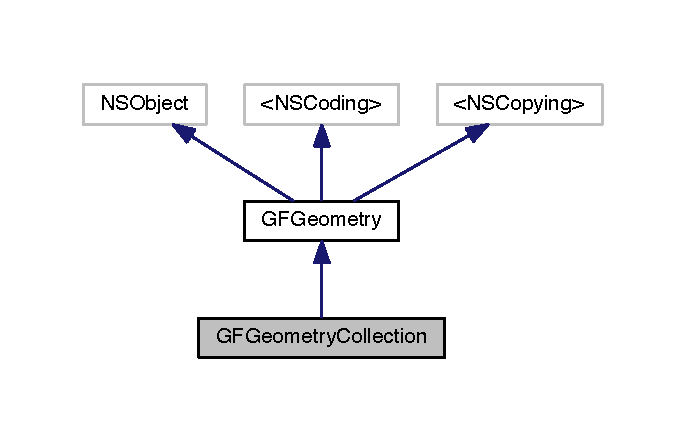
\includegraphics[width=329pt]{interface_g_f_geometry_collection__inherit__graph}
\end{center}
\end{figure}


Collaboration diagram for G\+F\+Geometry\+Collection\+:\nopagebreak
\begin{figure}[H]
\begin{center}
\leavevmode
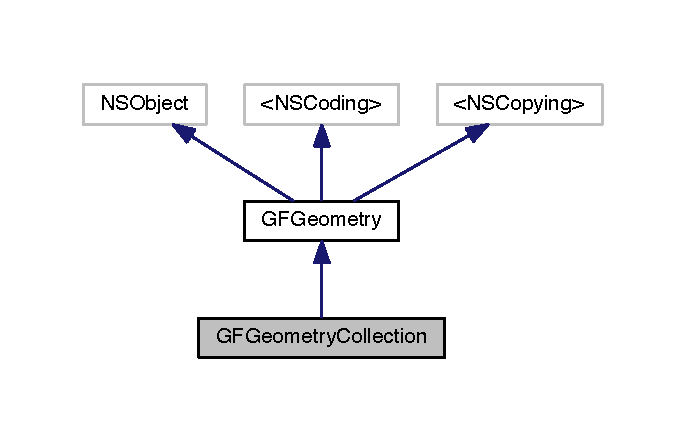
\includegraphics[width=329pt]{interface_g_f_geometry_collection__coll__graph}
\end{center}
\end{figure}
\subsection*{Instance Methods}
\begin{DoxyCompactItemize}
\item 
(instancetype) -\/ \hyperlink{interface_g_f_geometry_collection_a260bb3daa9d3324cb1cc2fa9ef3a61e9}{init\+With\+Array\+:}
\item 
(N\+S\+U\+Integer) -\/ \hyperlink{interface_g_f_geometry_collection_a020dd5245b572a391ccbd1ea92699240}{count}
\item 
(\hyperlink{interface_g_f_geometry}{G\+F\+Geometry} $\ast$) -\/ \hyperlink{interface_g_f_geometry_collection_aa4a654ef8751bdf8abac169f8746d026}{geometry\+At\+Index\+:}
\item 
(\hyperlink{interface_g_f_geometry}{G\+F\+Geometry} $\ast$) -\/ \hyperlink{interface_g_f_geometry_collection_a1910e3af2895a6c9cb7baf18ec791aad}{first\+Geometry}
\item 
(\hyperlink{interface_g_f_geometry}{G\+F\+Geometry} $\ast$) -\/ \hyperlink{interface_g_f_geometry_collection_a46262687af8b3c6599b2b2d68b0481b6}{last\+Geometry}
\end{DoxyCompactItemize}
\subsection*{Additional Inherited Members}


\subsection{Detailed Description}
A container class containing an array of \hyperlink{interface_g_f_geometry}{G\+F\+Geometry} objects. 

\begin{DoxyAuthor}{Author}
Tony Stone 
\end{DoxyAuthor}
\begin{DoxyDate}{Date}
6/5/15 
\end{DoxyDate}


\subsection{Method Documentation}
\hypertarget{interface_g_f_geometry_collection_a260bb3daa9d3324cb1cc2fa9ef3a61e9}{}\index{G\+F\+Geometry\+Collection@{G\+F\+Geometry\+Collection}!init\+With\+Array\+:@{init\+With\+Array\+:}}
\index{init\+With\+Array\+:@{init\+With\+Array\+:}!G\+F\+Geometry\+Collection@{G\+F\+Geometry\+Collection}}
\subsubsection[{init\+With\+Array\+:(\+N\+S\+Array $\ast$array)}]{\setlength{\rightskip}{0pt plus 5cm}-\/ (instancetype) init\+With\+Array\+: 
\begin{DoxyParamCaption}
\item[{(N\+S\+Array $\ast$)}]{array}
\end{DoxyParamCaption}
}\label{interface_g_f_geometry_collection_a260bb3daa9d3324cb1cc2fa9ef3a61e9}
Initialize this \hyperlink{interface_g_f_geometry_collection}{G\+F\+Geometry\+Collection} with the N\+S\+Array of \hyperlink{interface_g_f_geometry}{G\+F\+Geometry} instances.

\begin{DoxyWarning}{Warning}
The array must not contain another \hyperlink{interface_g_f_geometry_collection}{G\+F\+Geometry\+Collection} instance. 
\end{DoxyWarning}
\hypertarget{interface_g_f_geometry_collection_a020dd5245b572a391ccbd1ea92699240}{}\index{G\+F\+Geometry\+Collection@{G\+F\+Geometry\+Collection}!count@{count}}
\index{count@{count}!G\+F\+Geometry\+Collection@{G\+F\+Geometry\+Collection}}
\subsubsection[{count()}]{\setlength{\rightskip}{0pt plus 5cm}-\/ (N\+S\+U\+Integer) count 
\begin{DoxyParamCaption}
{}
\end{DoxyParamCaption}
}\label{interface_g_f_geometry_collection_a020dd5245b572a391ccbd1ea92699240}
\begin{DoxyReturn}{Returns}
The count of G\+D\+Geometry instances this collection contains. 
\end{DoxyReturn}
\hypertarget{interface_g_f_geometry_collection_aa4a654ef8751bdf8abac169f8746d026}{}\index{G\+F\+Geometry\+Collection@{G\+F\+Geometry\+Collection}!geometry\+At\+Index\+:@{geometry\+At\+Index\+:}}
\index{geometry\+At\+Index\+:@{geometry\+At\+Index\+:}!G\+F\+Geometry\+Collection@{G\+F\+Geometry\+Collection}}
\subsubsection[{geometry\+At\+Index\+:(\+N\+S\+U\+Integer index)}]{\setlength{\rightskip}{0pt plus 5cm}-\/ ({\bf G\+F\+Geometry} $\ast$) geometry\+At\+Index\+: 
\begin{DoxyParamCaption}
\item[{(N\+S\+U\+Integer)}]{index}
\end{DoxyParamCaption}
}\label{interface_g_f_geometry_collection_aa4a654ef8751bdf8abac169f8746d026}
\begin{DoxyReturn}{Returns}
The \hyperlink{interface_g_f_geometry}{G\+F\+Geometry} instance at the index given. 
\end{DoxyReturn}
\hypertarget{interface_g_f_geometry_collection_a1910e3af2895a6c9cb7baf18ec791aad}{}\index{G\+F\+Geometry\+Collection@{G\+F\+Geometry\+Collection}!first\+Geometry@{first\+Geometry}}
\index{first\+Geometry@{first\+Geometry}!G\+F\+Geometry\+Collection@{G\+F\+Geometry\+Collection}}
\subsubsection[{first\+Geometry()}]{\setlength{\rightskip}{0pt plus 5cm}-\/ ({\bf G\+F\+Geometry} $\ast$) first\+Geometry 
\begin{DoxyParamCaption}
{}
\end{DoxyParamCaption}
}\label{interface_g_f_geometry_collection_a1910e3af2895a6c9cb7baf18ec791aad}
\begin{DoxyReturn}{Returns}
The first \hyperlink{interface_g_f_geometry}{G\+F\+Geometry} instances contained in this collection or nil if the container is empty. 
\end{DoxyReturn}
\hypertarget{interface_g_f_geometry_collection_a46262687af8b3c6599b2b2d68b0481b6}{}\index{G\+F\+Geometry\+Collection@{G\+F\+Geometry\+Collection}!last\+Geometry@{last\+Geometry}}
\index{last\+Geometry@{last\+Geometry}!G\+F\+Geometry\+Collection@{G\+F\+Geometry\+Collection}}
\subsubsection[{last\+Geometry()}]{\setlength{\rightskip}{0pt plus 5cm}-\/ ({\bf G\+F\+Geometry} $\ast$) last\+Geometry 
\begin{DoxyParamCaption}
{}
\end{DoxyParamCaption}
}\label{interface_g_f_geometry_collection_a46262687af8b3c6599b2b2d68b0481b6}
\begin{DoxyReturn}{Returns}
The last \hyperlink{interface_g_f_geometry}{G\+F\+Geometry} instances contained in this collection or nil if the container is empty. 
\end{DoxyReturn}


The documentation for this class was generated from the following file\+:\begin{DoxyCompactItemize}
\item 
Geo\+Features/G\+F\+Geometry\+Collection.\+h\end{DoxyCompactItemize}

\hypertarget{interface_g_f_line_string}{}\section{G\+F\+Line\+String Class Reference}
\label{interface_g_f_line_string}\index{G\+F\+Line\+String@{G\+F\+Line\+String}}


A \hyperlink{interface_g_f_line_string}{G\+F\+Line\+String} is a collection of G\+F\+Points.  




{\ttfamily \#import $<$Geo\+Features/\+G\+F\+Line\+String.\+h$>$}



Inheritance diagram for G\+F\+Line\+String\+:\nopagebreak
\begin{figure}[H]
\begin{center}
\leavevmode
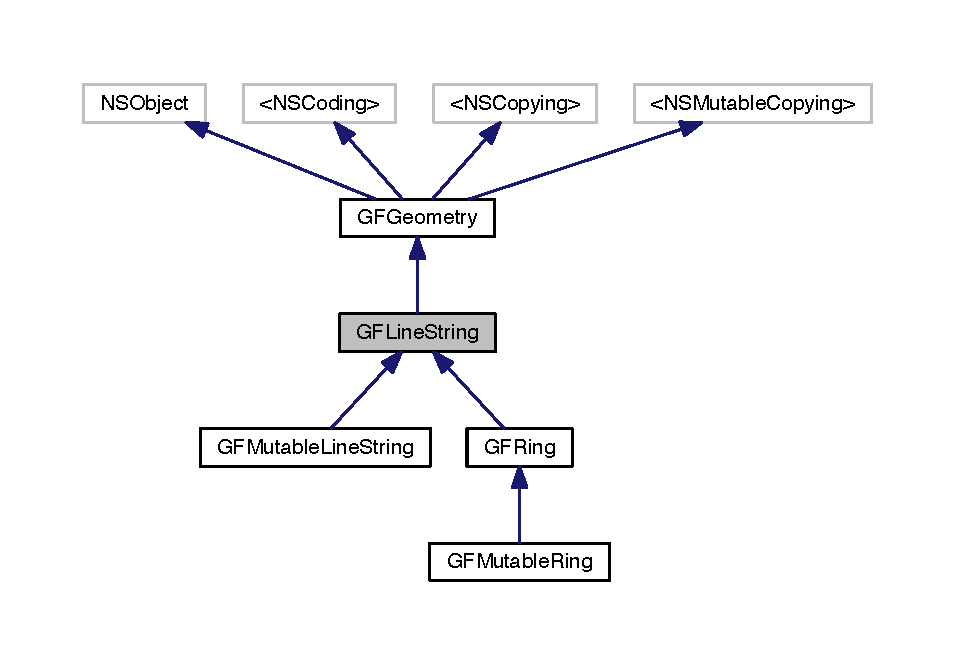
\includegraphics[width=329pt]{interface_g_f_line_string__inherit__graph}
\end{center}
\end{figure}


Collaboration diagram for G\+F\+Line\+String\+:\nopagebreak
\begin{figure}[H]
\begin{center}
\leavevmode
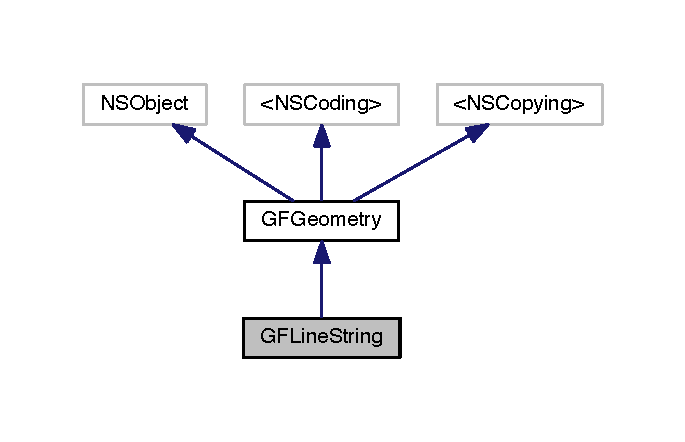
\includegraphics[width=329pt]{interface_g_f_line_string__coll__graph}
\end{center}
\end{figure}
\subsection*{Instance Methods}
\begin{DoxyCompactItemize}
\item 
(id) -\/ \hyperlink{interface_g_f_line_string_ae2adf99cdccb6ee23e22bd8e035d7896}{init\+With\+W\+K\+T\+:}
\item 
(id) -\/ \hyperlink{interface_g_f_line_string_a956fe6e6daf06ca4e016f94d18b2c71f}{init\+With\+Geo\+J\+S\+O\+N\+Geometry\+:}
\end{DoxyCompactItemize}
\subsection*{Additional Inherited Members}


\subsection{Detailed Description}
A \hyperlink{interface_g_f_line_string}{G\+F\+Line\+String} is a collection of G\+F\+Points. 

\begin{DoxyAuthor}{Author}
Tony Stone 
\end{DoxyAuthor}
\begin{DoxyDate}{Date}
6/14/15 
\end{DoxyDate}


\subsection{Method Documentation}
\hypertarget{interface_g_f_line_string_ae2adf99cdccb6ee23e22bd8e035d7896}{}\index{G\+F\+Line\+String@{G\+F\+Line\+String}!init\+With\+W\+K\+T\+:@{init\+With\+W\+K\+T\+:}}
\index{init\+With\+W\+K\+T\+:@{init\+With\+W\+K\+T\+:}!G\+F\+Line\+String@{G\+F\+Line\+String}}
\subsubsection[{init\+With\+W\+K\+T\+:(\+N\+S\+String $\ast$wkt)}]{\setlength{\rightskip}{0pt plus 5cm}-\/ (id) init\+With\+W\+K\+T\+: 
\begin{DoxyParamCaption}
\item[{(N\+S\+String $\ast$)}]{wkt}
\end{DoxyParamCaption}
}\label{interface_g_f_line_string_ae2adf99cdccb6ee23e22bd8e035d7896}
Initialize this geometry with the given W\+K\+T (Well-\/\+Known-\/\+Text) string.

Example\+: 
\begin{DoxyCode}
\{

  NSString * wkt = \textcolor{stringliteral}{@"LINESTRING(40 60,120 110)"};

  \hyperlink{interface_g_f_line_string}{GFLineString} * lineString = [[\hyperlink{interface_g_f_line_string}{GFLineString} alloc] initWithWKT: wkt]];

\}
\end{DoxyCode}
 \hypertarget{interface_g_f_line_string_a956fe6e6daf06ca4e016f94d18b2c71f}{}\index{G\+F\+Line\+String@{G\+F\+Line\+String}!init\+With\+Geo\+J\+S\+O\+N\+Geometry\+:@{init\+With\+Geo\+J\+S\+O\+N\+Geometry\+:}}
\index{init\+With\+Geo\+J\+S\+O\+N\+Geometry\+:@{init\+With\+Geo\+J\+S\+O\+N\+Geometry\+:}!G\+F\+Line\+String@{G\+F\+Line\+String}}
\subsubsection[{init\+With\+Geo\+J\+S\+O\+N\+Geometry\+:(\+N\+S\+Dictionary $\ast$json\+Dictionary)}]{\setlength{\rightskip}{0pt plus 5cm}-\/ (id) init\+With\+Geo\+J\+S\+O\+N\+Geometry\+: 
\begin{DoxyParamCaption}
\item[{(N\+S\+Dictionary $\ast$)}]{json\+Dictionary}
\end{DoxyParamCaption}
}\label{interface_g_f_line_string_a956fe6e6daf06ca4e016f94d18b2c71f}
Initialize this geometry with the given json\+Dictionary.

\begin{DoxyNote}{Note}


You must pass the geometry portion of the Geo\+J\+S\+O\+N structure and not the entire Geo\+J\+S\+O\+N object.

Example\+:


\begin{DoxyCode}
\{
      \textcolor{stringliteral}{"type"}: \textcolor{stringliteral}{"Feature"},

      \textcolor{stringliteral}{"geometry"}: \{ \textcolor{stringliteral}{"type"}: \textcolor{stringliteral}{"LineString"},
                    \textcolor{stringliteral}{"coordinates"}: [ [100.0, 0.0], [101.0, 1.0] ]
                  \}
 \}
\end{DoxyCode}


In the above example only the dictionary below that represents the geometry portion is passed.


\begin{DoxyCode}
\{
      \textcolor{stringliteral}{"type"}: \textcolor{stringliteral}{"LineString"},
      \textcolor{stringliteral}{"coordinates"}: [ [100.0, 0.0], [101.0, 1.0] ]
\}
\end{DoxyCode}
 
\end{DoxyNote}


The documentation for this class was generated from the following file\+:\begin{DoxyCompactItemize}
\item 
Geo\+Features/G\+F\+Line\+String.\+h\end{DoxyCompactItemize}

\hypertarget{interface_g_f_line_string_abstract}{}\section{G\+F\+Line\+String\+Abstract Class Reference}
\label{interface_g_f_line_string_abstract}\index{G\+F\+Line\+String\+Abstract@{G\+F\+Line\+String\+Abstract}}


An Abstract Line\+String implementation.  




{\ttfamily \#import $<$Geo\+Features/\+G\+F\+Line\+String\+Abstract.\+h$>$}



Inheritance diagram for G\+F\+Line\+String\+Abstract\+:
\nopagebreak
\begin{figure}[H]
\begin{center}
\leavevmode
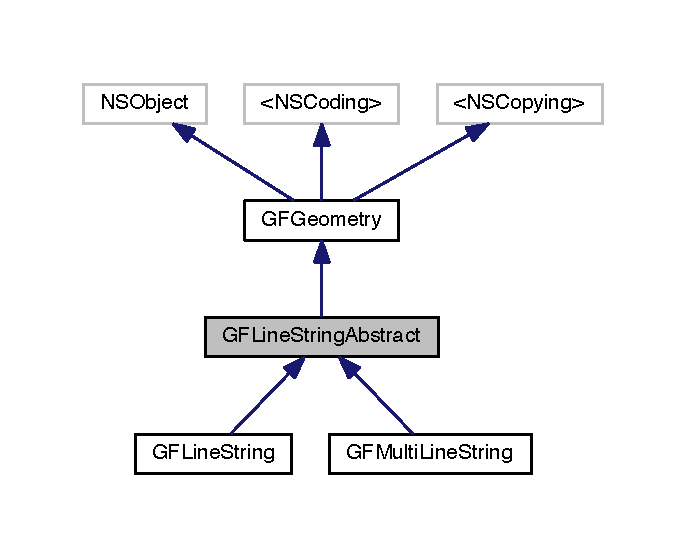
\includegraphics[width=350pt]{interface_g_f_line_string_abstract__inherit__graph}
\end{center}
\end{figure}


Collaboration diagram for G\+F\+Line\+String\+Abstract\+:
\nopagebreak
\begin{figure}[H]
\begin{center}
\leavevmode
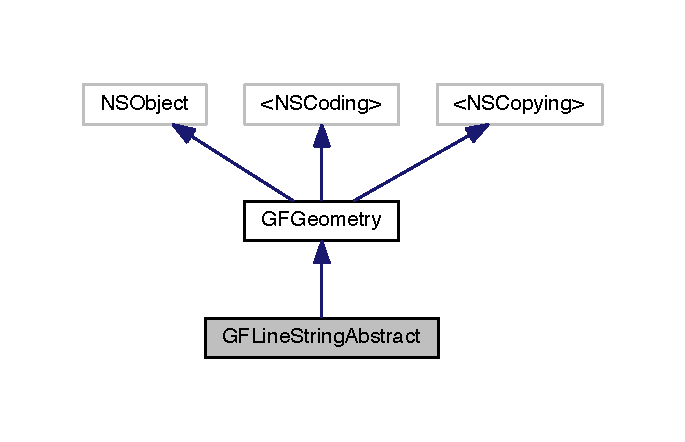
\includegraphics[width=350pt]{interface_g_f_line_string_abstract__coll__graph}
\end{center}
\end{figure}
\subsection*{Additional Inherited Members}


\subsection{Detailed Description}
An Abstract Line\+String implementation. 

An Abstract Line\+String implementation which should not be instantiated on it\textquotesingle{}s own.

\begin{DoxyWarning}{Warning}
Do not instantiate this abstract class.
\end{DoxyWarning}
\begin{DoxyRefDesc}{Deprecated}
\item[\hyperlink{deprecated__deprecated000001}{Deprecated}]This class will be removed in v2, please don\textquotesingle{}t directly rely on it at this point.\end{DoxyRefDesc}


\begin{DoxyAuthor}{Author}
Tony Stone 
\end{DoxyAuthor}
\begin{DoxyDate}{Date}
6/6/15 
\end{DoxyDate}


The documentation for this class was generated from the following file\+:\begin{DoxyCompactItemize}
\item 
Geo\+Features/G\+F\+Line\+String\+Abstract.\+h\end{DoxyCompactItemize}

\hypertarget{interface_g_f_multi_line_string}{}\section{G\+F\+Multi\+Line\+String Class Reference}
\label{interface_g_f_multi_line_string}\index{G\+F\+Multi\+Line\+String@{G\+F\+Multi\+Line\+String}}


A collection of G\+F\+Line\+Strings.  




{\ttfamily \#import $<$Geo\+Features/\+G\+F\+Multi\+Line\+String.\+h$>$}



Inheritance diagram for G\+F\+Multi\+Line\+String\+:
\nopagebreak
\begin{figure}[H]
\begin{center}
\leavevmode
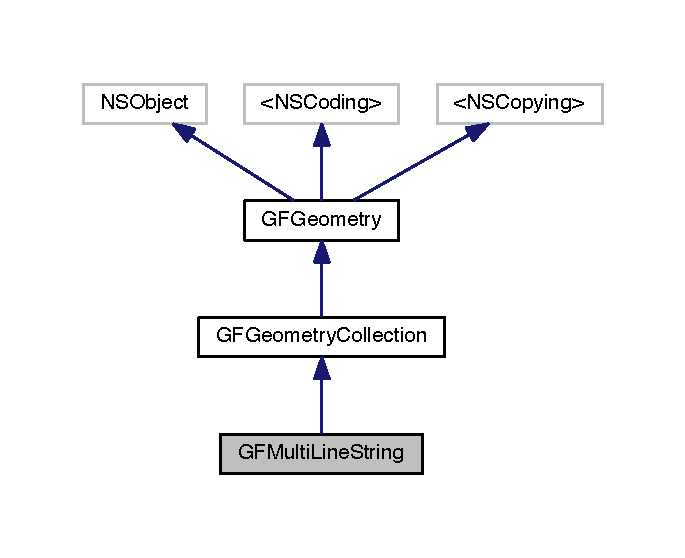
\includegraphics[width=350pt]{interface_g_f_multi_line_string__inherit__graph}
\end{center}
\end{figure}


Collaboration diagram for G\+F\+Multi\+Line\+String\+:
\nopagebreak
\begin{figure}[H]
\begin{center}
\leavevmode
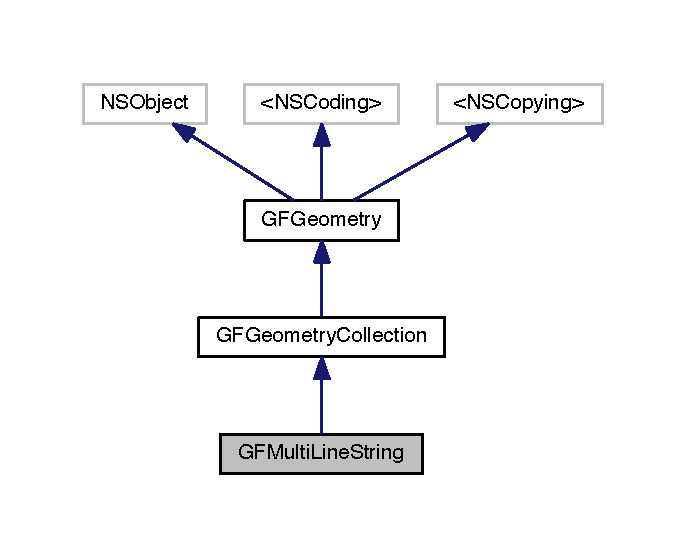
\includegraphics[width=350pt]{interface_g_f_multi_line_string__coll__graph}
\end{center}
\end{figure}
\subsection*{Instance Methods}
\begin{DoxyCompactItemize}
\item 
(instancetype) -\/ \hyperlink{interface_g_f_multi_line_string_a23cca8dc30634c3ac23c8cfaca41c569}{init\+With\+W\+K\+T\+:}
\item 
(instancetype) -\/ \hyperlink{interface_g_f_multi_line_string_a35fba00c08f785e70b47dda5067f84f8}{init\+With\+Geo\+J\+S\+O\+N\+Geometry\+:}
\item 
(N\+S\+U\+Integer) -\/ \hyperlink{interface_g_f_multi_line_string_a49494350a429df86186d111b5496d66c}{count}
\item 
(\hyperlink{interface_g_f_line_string}{G\+F\+Line\+String} $\ast$) -\/ \hyperlink{interface_g_f_multi_line_string_a6724df65ee49b15e8778f965d3498bcb}{geometry\+At\+Index\+:}
\item 
(\hyperlink{interface_g_f_line_string}{G\+F\+Line\+String} $\ast$) -\/ \hyperlink{interface_g_f_multi_line_string_a78586818fa6ddbce9c3cf2032eba7f2d}{first\+Geometry}
\item 
(\hyperlink{interface_g_f_line_string}{G\+F\+Line\+String} $\ast$) -\/ \hyperlink{interface_g_f_multi_line_string_a807c900c20062193febb780e4ecc6abd}{last\+Geometry}
\item 
(\hyperlink{interface_g_f_line_string}{G\+F\+Line\+String} $\ast$) -\/ \hyperlink{interface_g_f_multi_line_string_a00496d2af8be614fe4cc11c6a6347591}{object\+At\+Indexed\+Subscript\+:}
\end{DoxyCompactItemize}
\subsection*{Additional Inherited Members}


\subsection{Detailed Description}
A collection of G\+F\+Line\+Strings. 

Multi\+Line\+String can be used to group lines belonging to each other, e.\+g. a highway (with interruptions)

\begin{DoxyAuthor}{Author}
Tony Stone 
\end{DoxyAuthor}
\begin{DoxyDate}{Date}
6/4/15 
\end{DoxyDate}


\subsection{Method Documentation}
\hypertarget{interface_g_f_multi_line_string_a23cca8dc30634c3ac23c8cfaca41c569}{}\index{G\+F\+Multi\+Line\+String@{G\+F\+Multi\+Line\+String}!init\+With\+W\+K\+T\+:@{init\+With\+W\+K\+T\+:}}
\index{init\+With\+W\+K\+T\+:@{init\+With\+W\+K\+T\+:}!G\+F\+Multi\+Line\+String@{G\+F\+Multi\+Line\+String}}
\subsubsection[{init\+With\+W\+K\+T\+:(\+N\+S\+String $\ast$wkt)}]{\setlength{\rightskip}{0pt plus 5cm}-\/ (instancetype) init\+With\+W\+K\+T\+: 
\begin{DoxyParamCaption}
\item[{(N\+S\+String $\ast$)}]{wkt}
\end{DoxyParamCaption}
}\label{interface_g_f_multi_line_string_a23cca8dc30634c3ac23c8cfaca41c569}
Initialize this geometry with the given W\+K\+T (Well-\/\+Known-\/\+Text) string.

Example\+: 
\begin{DoxyCode}
\{

  NSString * wkt = \textcolor{stringliteral}{@"MULTILINESTRING((0 0,5 0),(5 0,10 0,5 -5,5 0),(5 0,5 5))"};

  \hyperlink{interface_g_f_multi_line_string}{GFMultiLineString} * multiLineString = [[\hyperlink{interface_g_f_multi_line_string}{GFMultiLineString} alloc] 
      initWithWKT: wkt]];

\}
\end{DoxyCode}
 

Reimplemented from \hyperlink{interface_g_f_geometry_collection_a13156620e5298fe7d286bb800df4097b}{G\+F\+Geometry\+Collection}.

\hypertarget{interface_g_f_multi_line_string_a35fba00c08f785e70b47dda5067f84f8}{}\index{G\+F\+Multi\+Line\+String@{G\+F\+Multi\+Line\+String}!init\+With\+Geo\+J\+S\+O\+N\+Geometry\+:@{init\+With\+Geo\+J\+S\+O\+N\+Geometry\+:}}
\index{init\+With\+Geo\+J\+S\+O\+N\+Geometry\+:@{init\+With\+Geo\+J\+S\+O\+N\+Geometry\+:}!G\+F\+Multi\+Line\+String@{G\+F\+Multi\+Line\+String}}
\subsubsection[{init\+With\+Geo\+J\+S\+O\+N\+Geometry\+:(\+N\+S\+Dictionary $\ast$json\+Dictionary)}]{\setlength{\rightskip}{0pt plus 5cm}-\/ (instancetype) init\+With\+Geo\+J\+S\+O\+N\+Geometry\+: 
\begin{DoxyParamCaption}
\item[{(N\+S\+Dictionary $\ast$)}]{json\+Dictionary}
\end{DoxyParamCaption}
}\label{interface_g_f_multi_line_string_a35fba00c08f785e70b47dda5067f84f8}
Initialize this geometry with the given json\+Dictionary.

\begin{DoxyNote}{Note}


You must pass the geometry portion of the Geo\+J\+S\+O\+N structure and not the entire Geo\+J\+S\+O\+N object.

Example\+:


\begin{DoxyCode}
\{
      \textcolor{stringliteral}{"type"}: \textcolor{stringliteral}{"Feature"},

      \textcolor{stringliteral}{"geometry"}: \{ \textcolor{stringliteral}{"type"}: \textcolor{stringliteral}{"MultiLineString"},
                    \textcolor{stringliteral}{"coordinates"}: [
                              [ [100.0, 0.0], [101.0, 1.0] ],
                              [ [102.0, 2.0], [103.0, 3.0] ]
                      ]
                  \}
 \}
\end{DoxyCode}


In the above example only the dictionary below that represents the geometry portion is passed.


\begin{DoxyCode}
\{
    \textcolor{stringliteral}{"type"}: \textcolor{stringliteral}{"MultiLineString"},
    \textcolor{stringliteral}{"coordinates"}: [
            [ [100.0, 0.0], [101.0, 1.0] ],
            [ [102.0, 2.0], [103.0, 3.0] ]
      ]
\}
\end{DoxyCode}
 
\end{DoxyNote}
\hypertarget{interface_g_f_multi_line_string_a49494350a429df86186d111b5496d66c}{}\index{G\+F\+Multi\+Line\+String@{G\+F\+Multi\+Line\+String}!count@{count}}
\index{count@{count}!G\+F\+Multi\+Line\+String@{G\+F\+Multi\+Line\+String}}
\subsubsection[{count()}]{\setlength{\rightskip}{0pt plus 5cm}-\/ (N\+S\+U\+Integer) count 
\begin{DoxyParamCaption}
{}
\end{DoxyParamCaption}
}\label{interface_g_f_multi_line_string_a49494350a429df86186d111b5496d66c}
The number of \hyperlink{interface_g_f_line_string}{G\+F\+Line\+String} instances in this collection.

\begin{DoxyReturn}{Returns}
The count of \hyperlink{interface_g_f_line_string}{G\+F\+Line\+String} instances this collection contains.
\end{DoxyReturn}
\begin{DoxySince}{Since}
1.\+1.\+0 
\end{DoxySince}


Reimplemented from \hyperlink{interface_g_f_geometry_collection_a020dd5245b572a391ccbd1ea92699240}{G\+F\+Geometry\+Collection}.

\hypertarget{interface_g_f_multi_line_string_a6724df65ee49b15e8778f965d3498bcb}{}\index{G\+F\+Multi\+Line\+String@{G\+F\+Multi\+Line\+String}!geometry\+At\+Index\+:@{geometry\+At\+Index\+:}}
\index{geometry\+At\+Index\+:@{geometry\+At\+Index\+:}!G\+F\+Multi\+Line\+String@{G\+F\+Multi\+Line\+String}}
\subsubsection[{geometry\+At\+Index\+:(\+N\+S\+U\+Integer index)}]{\setlength{\rightskip}{0pt plus 5cm}-\/ ({\bf G\+F\+Line\+String} $\ast$) geometry\+At\+Index\+: 
\begin{DoxyParamCaption}
\item[{(N\+S\+U\+Integer)}]{index}
\end{DoxyParamCaption}
}\label{interface_g_f_multi_line_string_a6724df65ee49b15e8778f965d3498bcb}
Returns the \hyperlink{interface_g_f_line_string}{G\+F\+Line\+String} located at the specified index.


\begin{DoxyParams}{Parameters}
{\em index} & -\/ An index within the bounds of the collection.\\
\hline
\end{DoxyParams}
\begin{DoxyReturn}{Returns}
The \hyperlink{interface_g_f_line_string}{G\+F\+Line\+String} located at index.
\end{DoxyReturn}

\begin{DoxyExceptions}{Exceptions}
{\em N\+S\+Exception,N\+S\+Range\+Exception} & If index is beyond the end of the collection (that is, if index is greater than or equal to the value returned by count), an N\+S\+Range\+Exception is raised.\\
\hline
\end{DoxyExceptions}
\begin{DoxySince}{Since}
1.\+1.\+0 
\end{DoxySince}


Reimplemented from \hyperlink{interface_g_f_geometry_collection_a4cd182279facec2850b47634aa0f6297}{G\+F\+Geometry\+Collection}.

\hypertarget{interface_g_f_multi_line_string_a78586818fa6ddbce9c3cf2032eba7f2d}{}\index{G\+F\+Multi\+Line\+String@{G\+F\+Multi\+Line\+String}!first\+Geometry@{first\+Geometry}}
\index{first\+Geometry@{first\+Geometry}!G\+F\+Multi\+Line\+String@{G\+F\+Multi\+Line\+String}}
\subsubsection[{first\+Geometry()}]{\setlength{\rightskip}{0pt plus 5cm}-\/ ({\bf G\+F\+Line\+String} $\ast$) first\+Geometry 
\begin{DoxyParamCaption}
{}
\end{DoxyParamCaption}
}\label{interface_g_f_multi_line_string_a78586818fa6ddbce9c3cf2032eba7f2d}
The first \hyperlink{interface_g_f_line_string}{G\+F\+Line\+String} in this collection.

\begin{DoxyReturn}{Returns}
The first \hyperlink{interface_g_f_line_string}{G\+F\+Line\+String} instances contained in this collection or nil if the container is empty.
\end{DoxyReturn}
\begin{DoxySince}{Since}
1.\+1.\+0 
\end{DoxySince}


Reimplemented from \hyperlink{interface_g_f_geometry_collection_a610f72a22d76a3ce6c9eaeb2dad35c0e}{G\+F\+Geometry\+Collection}.

\hypertarget{interface_g_f_multi_line_string_a807c900c20062193febb780e4ecc6abd}{}\index{G\+F\+Multi\+Line\+String@{G\+F\+Multi\+Line\+String}!last\+Geometry@{last\+Geometry}}
\index{last\+Geometry@{last\+Geometry}!G\+F\+Multi\+Line\+String@{G\+F\+Multi\+Line\+String}}
\subsubsection[{last\+Geometry()}]{\setlength{\rightskip}{0pt plus 5cm}-\/ ({\bf G\+F\+Line\+String} $\ast$) last\+Geometry 
\begin{DoxyParamCaption}
{}
\end{DoxyParamCaption}
}\label{interface_g_f_multi_line_string_a807c900c20062193febb780e4ecc6abd}
The last \hyperlink{interface_g_f_line_string}{G\+F\+Line\+String} in this collection.

\begin{DoxyReturn}{Returns}
The last \hyperlink{interface_g_f_line_string}{G\+F\+Line\+String} instances contained in this collection or nil if the container is empty.
\end{DoxyReturn}
\begin{DoxySince}{Since}
1.\+1.\+0 
\end{DoxySince}


Reimplemented from \hyperlink{interface_g_f_geometry_collection_a89b3b6e2097cf5899a6d635ddcb95ef3}{G\+F\+Geometry\+Collection}.

\hypertarget{interface_g_f_multi_line_string_a00496d2af8be614fe4cc11c6a6347591}{}\index{G\+F\+Multi\+Line\+String@{G\+F\+Multi\+Line\+String}!object\+At\+Indexed\+Subscript\+:@{object\+At\+Indexed\+Subscript\+:}}
\index{object\+At\+Indexed\+Subscript\+:@{object\+At\+Indexed\+Subscript\+:}!G\+F\+Multi\+Line\+String@{G\+F\+Multi\+Line\+String}}
\subsubsection[{object\+At\+Indexed\+Subscript\+:(\+N\+S\+U\+Integer index)}]{\setlength{\rightskip}{0pt plus 5cm}-\/ ({\bf G\+F\+Line\+String} $\ast$) object\+At\+Indexed\+Subscript\+: 
\begin{DoxyParamCaption}
\item[{(N\+S\+U\+Integer)}]{index}
\end{DoxyParamCaption}
}\label{interface_g_f_multi_line_string_a00496d2af8be614fe4cc11c6a6347591}
Returns the \hyperlink{interface_g_f_line_string}{G\+F\+Line\+String} at the specified index.


\begin{DoxyParams}{Parameters}
{\em index} & An index within the bounds of the collection.\\
\hline
\end{DoxyParams}
\begin{DoxyReturn}{Returns}
The \hyperlink{interface_g_f_line_string}{G\+F\+Line\+String} located at index.
\end{DoxyReturn}
Example\+:


\begin{DoxyCode}
\{
   \hyperlink{interface_g_f_multi_line_string}{GFMultiLineString} * multiLineString = [[\hyperlink{interface_g_f_multi_line_string}{GFMultiLineString} alloc] 
      initWithWKT: \textcolor{stringliteral}{@"MULTILINESTRING((0 0,5 0),(5 0,10 0,5 -5,5 0),(5 0,5 5))"}];

   \hyperlink{interface_g_f_line_string}{GFLineString} * lineString = multiLineString[1];
\}
\end{DoxyCode}



\begin{DoxyExceptions}{Exceptions}
{\em N\+S\+Exception} & If index is beyond the end of the collection (that is, if index is greater than or equal to the value returned by count), an N\+S\+Range\+Exception is raised.\\
\hline
\end{DoxyExceptions}
\begin{DoxySince}{Since}
1.\+1.\+0 
\end{DoxySince}


Reimplemented from \hyperlink{interface_g_f_geometry_collection_ac67dd4526580a8a38408e39c489a7503}{G\+F\+Geometry\+Collection}.



The documentation for this class was generated from the following file\+:\begin{DoxyCompactItemize}
\item 
Geo\+Features/G\+F\+Multi\+Line\+String.\+h\end{DoxyCompactItemize}

\hypertarget{interface_g_f_multi_point}{}\section{G\+F\+Multi\+Point Class Reference}
\label{interface_g_f_multi_point}\index{G\+F\+Multi\+Point@{G\+F\+Multi\+Point}}


A collection of G\+F\+Points.  




{\ttfamily \#import $<$Geo\+Features/\+G\+F\+Multi\+Point.\+h$>$}



Inheritance diagram for G\+F\+Multi\+Point\+:\nopagebreak
\begin{figure}[H]
\begin{center}
\leavevmode
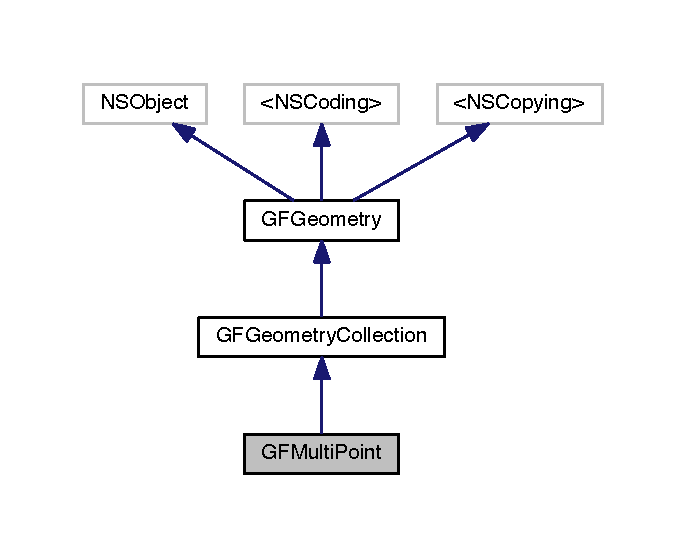
\includegraphics[width=350pt]{interface_g_f_multi_point__inherit__graph}
\end{center}
\end{figure}


Collaboration diagram for G\+F\+Multi\+Point\+:\nopagebreak
\begin{figure}[H]
\begin{center}
\leavevmode
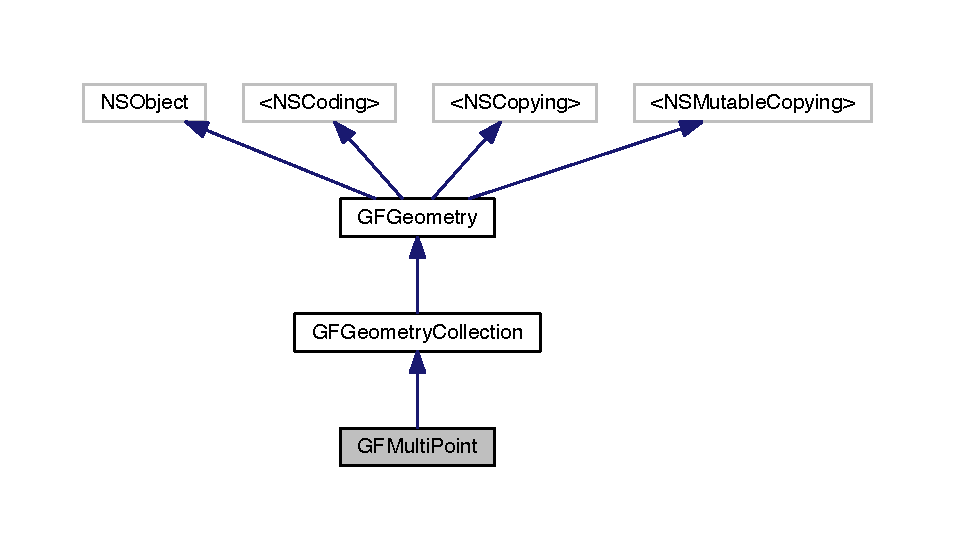
\includegraphics[width=350pt]{interface_g_f_multi_point__coll__graph}
\end{center}
\end{figure}
\subsection*{Instance Methods}
\begin{DoxyCompactItemize}
\item 
(instancetype) -\/ \hyperlink{interface_g_f_multi_point_a003eb1cee88057991c210dd0cd63ef7f}{init\+With\+W\+K\+T\+:}
\item 
(instancetype) -\/ \hyperlink{interface_g_f_multi_point_a3da732dd6a2635ab6ac56abf24168829}{init\+With\+W\+K\+T\+:error\+:}
\item 
(instancetype) -\/ \hyperlink{interface_g_f_multi_point_a08bc62987b4e8c0435b00367dd617e00}{init\+With\+Geo\+J\+S\+O\+N\+Geometry\+:}
\item 
(instancetype) -\/ \hyperlink{interface_g_f_multi_point_aed5c1b63f03328cb0796d3be78f790b1}{init\+With\+Geo\+J\+S\+O\+N\+Geometry\+:error\+:}
\item 
(N\+S\+U\+Integer) -\/ \hyperlink{interface_g_f_multi_point_afb692f3668a3631fbec6739c7fd7bf2c}{count}
\item 
(\hyperlink{interface_g_f_point}{G\+F\+Point} $\ast$) -\/ \hyperlink{interface_g_f_multi_point_a679f88a16cfc5e7d2d2bd1fda95303be}{geometry\+At\+Index\+:}
\item 
(\hyperlink{interface_g_f_point}{G\+F\+Point} $\ast$) -\/ \hyperlink{interface_g_f_multi_point_a2f300bc57f0010bc65da0f151b916e33}{first\+Geometry}
\item 
(\hyperlink{interface_g_f_point}{G\+F\+Point} $\ast$) -\/ \hyperlink{interface_g_f_multi_point_aa0c216ccbac49420bb8694fdb3311c6b}{last\+Geometry}
\item 
(\hyperlink{interface_g_f_point}{G\+F\+Point} $\ast$) -\/ \hyperlink{interface_g_f_multi_point_a003241a11b6d6da14364bb8a07c05a35}{object\+At\+Indexed\+Subscript\+:}
\end{DoxyCompactItemize}
\subsection*{Additional Inherited Members}


\subsection{Detailed Description}
A collection of G\+F\+Points. 

\begin{DoxyAuthor}{Author}
Tony Stone 
\end{DoxyAuthor}
\begin{DoxyDate}{Date}
6/14/15 
\end{DoxyDate}


\subsection{Method Documentation}
\hypertarget{interface_g_f_multi_point_a003eb1cee88057991c210dd0cd63ef7f}{}\index{G\+F\+Multi\+Point@{G\+F\+Multi\+Point}!init\+With\+W\+K\+T\+:@{init\+With\+W\+K\+T\+:}}
\index{init\+With\+W\+K\+T\+:@{init\+With\+W\+K\+T\+:}!G\+F\+Multi\+Point@{G\+F\+Multi\+Point}}
\subsubsection[{init\+With\+W\+K\+T\+:(\+N\+S\+String $\ast$wkt)}]{\setlength{\rightskip}{0pt plus 5cm}-\/ (instancetype) init\+With\+W\+K\+T\+: 
\begin{DoxyParamCaption}
\item[{(N\+S\+String $\ast$)}]{wkt}
\end{DoxyParamCaption}
}\label{interface_g_f_multi_point_a003eb1cee88057991c210dd0cd63ef7f}
Initialize this geometry with the given W\+K\+T (Well-\/\+Known-\/\+Text) string.

Example\+: 
\begin{DoxyCode}
\{

  NSString * wkt = \textcolor{stringliteral}{@"MULTIPOINT((1 1),(2 2))"};

  \hyperlink{interface_g_f_multi_point}{GFMultiPoint} * multiPoint = [[\hyperlink{interface_g_f_multi_point}{GFMultiPoint} alloc] initWithWKT: wkt]];

\}
\end{DoxyCode}
 

Reimplemented from \hyperlink{interface_g_f_geometry_collection_a13156620e5298fe7d286bb800df4097b}{G\+F\+Geometry\+Collection}.

\hypertarget{interface_g_f_multi_point_a3da732dd6a2635ab6ac56abf24168829}{}\index{G\+F\+Multi\+Point@{G\+F\+Multi\+Point}!init\+With\+W\+K\+T\+:error\+:@{init\+With\+W\+K\+T\+:error\+:}}
\index{init\+With\+W\+K\+T\+:error\+:@{init\+With\+W\+K\+T\+:error\+:}!G\+F\+Multi\+Point@{G\+F\+Multi\+Point}}
\subsubsection[{init\+With\+W\+K\+T\+:error\+:(\+N\+S\+String $\ast$wkt,[error] N\+S\+Error $\ast$\+\_\+\+\_\+autoreleasing $\ast$error)}]{\setlength{\rightskip}{0pt plus 5cm}-\/ (instancetype) {\bf init\+With\+W\+K\+T\+:} 
\begin{DoxyParamCaption}
\item[{(N\+S\+String $\ast$)}]{wkt}
\item[{error:(N\+S\+Error $\ast$\+\_\+\+\_\+autoreleasing $\ast$)}]{error}
\end{DoxyParamCaption}
}\label{interface_g_f_multi_point_a3da732dd6a2635ab6ac56abf24168829}
Initialize this geometry with the given W\+K\+T (Well-\/\+Known-\/\+Text) string.

Example\+: 
\begin{DoxyCode}
\{

  NSString * wkt = \textcolor{stringliteral}{@"MULTIPOINT((1 1),(2 2))"};

  NSError * error = nil;

  \hyperlink{interface_g_f_multi_point}{GFMultiPoint} * multiPoint = [[\hyperlink{interface_g_f_multi_point}{GFMultiPoint} alloc] initWithWKT: wkt error: &error]
      ];

\}
\end{DoxyCode}
 

Reimplemented from \hyperlink{interface_g_f_geometry_collection_ab9106d38d85940ef0bfa6eeb89d90193}{G\+F\+Geometry\+Collection}.

\hypertarget{interface_g_f_multi_point_a08bc62987b4e8c0435b00367dd617e00}{}\index{G\+F\+Multi\+Point@{G\+F\+Multi\+Point}!init\+With\+Geo\+J\+S\+O\+N\+Geometry\+:@{init\+With\+Geo\+J\+S\+O\+N\+Geometry\+:}}
\index{init\+With\+Geo\+J\+S\+O\+N\+Geometry\+:@{init\+With\+Geo\+J\+S\+O\+N\+Geometry\+:}!G\+F\+Multi\+Point@{G\+F\+Multi\+Point}}
\subsubsection[{init\+With\+Geo\+J\+S\+O\+N\+Geometry\+:(\+N\+S\+Dictionary $\ast$json\+Dictionary)}]{\setlength{\rightskip}{0pt plus 5cm}-\/ (instancetype) init\+With\+Geo\+J\+S\+O\+N\+Geometry\+: 
\begin{DoxyParamCaption}
\item[{(N\+S\+Dictionary $\ast$)}]{json\+Dictionary}
\end{DoxyParamCaption}
}\label{interface_g_f_multi_point_a08bc62987b4e8c0435b00367dd617e00}
Initialize this geometry with the given json\+Dictionary.

\begin{DoxyNote}{Note}


You must pass the geometry portion of the Geo\+J\+S\+O\+N structure and not the entire Geo\+J\+S\+O\+N object.

Example\+:


\begin{DoxyCode}
\{
      \textcolor{stringliteral}{"type"}: \textcolor{stringliteral}{"Feature"},

      \textcolor{stringliteral}{"geometry"}: \{ \textcolor{stringliteral}{"type"}: \textcolor{stringliteral}{"MultiPoint"},
                    \textcolor{stringliteral}{"coordinates"}: [ [100.0, 0.0], [101.0, 1.0] ]
                  \}
 \}
\end{DoxyCode}


In the above example only the dictionary below that represents the geometry portion is passed.


\begin{DoxyCode}
\{
    \textcolor{stringliteral}{"type"}: \textcolor{stringliteral}{"MultiPoint"},
    \textcolor{stringliteral}{"coordinates"}: [ [100.0, 0.0], [101.0, 1.0] ]
\}
\end{DoxyCode}
 
\end{DoxyNote}


Reimplemented from \hyperlink{interface_g_f_geometry_collection_adc8a317a694f82808d1e02e53e300f8f}{G\+F\+Geometry\+Collection}.

\hypertarget{interface_g_f_multi_point_aed5c1b63f03328cb0796d3be78f790b1}{}\index{G\+F\+Multi\+Point@{G\+F\+Multi\+Point}!init\+With\+Geo\+J\+S\+O\+N\+Geometry\+:error\+:@{init\+With\+Geo\+J\+S\+O\+N\+Geometry\+:error\+:}}
\index{init\+With\+Geo\+J\+S\+O\+N\+Geometry\+:error\+:@{init\+With\+Geo\+J\+S\+O\+N\+Geometry\+:error\+:}!G\+F\+Multi\+Point@{G\+F\+Multi\+Point}}
\subsubsection[{init\+With\+Geo\+J\+S\+O\+N\+Geometry\+:error\+:(\+N\+S\+Dictionary $\ast$json\+Dictionary,[error] N\+S\+Error $\ast$\+\_\+\+\_\+autoreleasing $\ast$error)}]{\setlength{\rightskip}{0pt plus 5cm}-\/ (instancetype) {\bf init\+With\+Geo\+J\+S\+O\+N\+Geometry\+:} 
\begin{DoxyParamCaption}
\item[{(N\+S\+Dictionary $\ast$)}]{json\+Dictionary}
\item[{error:(N\+S\+Error $\ast$\+\_\+\+\_\+autoreleasing $\ast$)}]{error}
\end{DoxyParamCaption}
}\label{interface_g_f_multi_point_aed5c1b63f03328cb0796d3be78f790b1}
Initialize this geometry with the given json\+Dictionary.

\begin{DoxyNote}{Note}


You must pass the geometry portion of the Geo\+J\+S\+O\+N structure and not the entire Geo\+J\+S\+O\+N object.

Example\+:


\begin{DoxyCode}
\{
      \textcolor{stringliteral}{"type"}: \textcolor{stringliteral}{"Feature"},

      \textcolor{stringliteral}{"geometry"}: \{ \textcolor{stringliteral}{"type"}: \textcolor{stringliteral}{"MultiPoint"},
                    \textcolor{stringliteral}{"coordinates"}: [ [100.0, 0.0], [101.0, 1.0] ]
                  \}
 \}
\end{DoxyCode}


In the above example only the dictionary below that represents the geometry portion is passed.


\begin{DoxyCode}
\{
    \textcolor{stringliteral}{"type"}: \textcolor{stringliteral}{"MultiPoint"},
    \textcolor{stringliteral}{"coordinates"}: [ [100.0, 0.0], [101.0, 1.0] ]
\}
\end{DoxyCode}
 
\end{DoxyNote}


Reimplemented from \hyperlink{interface_g_f_geometry_collection_a74b596f60b3363bb9f06b06847cb086d}{G\+F\+Geometry\+Collection}.

\hypertarget{interface_g_f_multi_point_afb692f3668a3631fbec6739c7fd7bf2c}{}\index{G\+F\+Multi\+Point@{G\+F\+Multi\+Point}!count@{count}}
\index{count@{count}!G\+F\+Multi\+Point@{G\+F\+Multi\+Point}}
\subsubsection[{count()}]{\setlength{\rightskip}{0pt plus 5cm}-\/ (N\+S\+U\+Integer) count 
\begin{DoxyParamCaption}
{}
\end{DoxyParamCaption}
}\label{interface_g_f_multi_point_afb692f3668a3631fbec6739c7fd7bf2c}
The number of \hyperlink{interface_g_f_point}{G\+F\+Point} instances in this collection.

\begin{DoxyReturn}{Returns}
The count of G\+D\+Geometry instances this collection contains.
\end{DoxyReturn}
\begin{DoxySince}{Since}
1.\+1.\+0 
\end{DoxySince}


Reimplemented from \hyperlink{interface_g_f_geometry_collection_a020dd5245b572a391ccbd1ea92699240}{G\+F\+Geometry\+Collection}.

\hypertarget{interface_g_f_multi_point_a679f88a16cfc5e7d2d2bd1fda95303be}{}\index{G\+F\+Multi\+Point@{G\+F\+Multi\+Point}!geometry\+At\+Index\+:@{geometry\+At\+Index\+:}}
\index{geometry\+At\+Index\+:@{geometry\+At\+Index\+:}!G\+F\+Multi\+Point@{G\+F\+Multi\+Point}}
\subsubsection[{geometry\+At\+Index\+:(\+N\+S\+U\+Integer index)}]{\setlength{\rightskip}{0pt plus 5cm}-\/ ({\bf G\+F\+Point} $\ast$) geometry\+At\+Index\+: 
\begin{DoxyParamCaption}
\item[{(N\+S\+U\+Integer)}]{index}
\end{DoxyParamCaption}
}\label{interface_g_f_multi_point_a679f88a16cfc5e7d2d2bd1fda95303be}
Returns the \hyperlink{interface_g_f_point}{G\+F\+Point} located at the specified index.


\begin{DoxyParams}{Parameters}
{\em index} & -\/ An index within the bounds of the collection.\\
\hline
\end{DoxyParams}
\begin{DoxyReturn}{Returns}
The \hyperlink{interface_g_f_point}{G\+F\+Point} located at index.
\end{DoxyReturn}

\begin{DoxyExceptions}{Exceptions}
{\em N\+S\+Exception,N\+S\+Range\+Exception} & If index is beyond the end of the collection (that is, if index is greater than or equal to the value returned by count), an N\+S\+Range\+Exception is raised.\\
\hline
\end{DoxyExceptions}
\begin{DoxySince}{Since}
1.\+1.\+0 
\end{DoxySince}


Reimplemented from \hyperlink{interface_g_f_geometry_collection_a4cd182279facec2850b47634aa0f6297}{G\+F\+Geometry\+Collection}.

\hypertarget{interface_g_f_multi_point_a2f300bc57f0010bc65da0f151b916e33}{}\index{G\+F\+Multi\+Point@{G\+F\+Multi\+Point}!first\+Geometry@{first\+Geometry}}
\index{first\+Geometry@{first\+Geometry}!G\+F\+Multi\+Point@{G\+F\+Multi\+Point}}
\subsubsection[{first\+Geometry()}]{\setlength{\rightskip}{0pt plus 5cm}-\/ ({\bf G\+F\+Point} $\ast$) first\+Geometry 
\begin{DoxyParamCaption}
{}
\end{DoxyParamCaption}
}\label{interface_g_f_multi_point_a2f300bc57f0010bc65da0f151b916e33}
The first \hyperlink{interface_g_f_point}{G\+F\+Point} in this collection.

\begin{DoxyReturn}{Returns}
The first \hyperlink{interface_g_f_point}{G\+F\+Point} instances contained in this collection or nil if the container is empty.
\end{DoxyReturn}
\begin{DoxySince}{Since}
1.\+1.\+0 
\end{DoxySince}


Reimplemented from \hyperlink{interface_g_f_geometry_collection_a610f72a22d76a3ce6c9eaeb2dad35c0e}{G\+F\+Geometry\+Collection}.

\hypertarget{interface_g_f_multi_point_aa0c216ccbac49420bb8694fdb3311c6b}{}\index{G\+F\+Multi\+Point@{G\+F\+Multi\+Point}!last\+Geometry@{last\+Geometry}}
\index{last\+Geometry@{last\+Geometry}!G\+F\+Multi\+Point@{G\+F\+Multi\+Point}}
\subsubsection[{last\+Geometry()}]{\setlength{\rightskip}{0pt plus 5cm}-\/ ({\bf G\+F\+Point} $\ast$) last\+Geometry 
\begin{DoxyParamCaption}
{}
\end{DoxyParamCaption}
}\label{interface_g_f_multi_point_aa0c216ccbac49420bb8694fdb3311c6b}
The last \hyperlink{interface_g_f_point}{G\+F\+Point} in this collection.

\begin{DoxyReturn}{Returns}
The last \hyperlink{interface_g_f_point}{G\+F\+Point} instances contained in this collection or nil if the container is empty.
\end{DoxyReturn}
\begin{DoxySince}{Since}
1.\+1.\+0 
\end{DoxySince}


Reimplemented from \hyperlink{interface_g_f_geometry_collection_a89b3b6e2097cf5899a6d635ddcb95ef3}{G\+F\+Geometry\+Collection}.

\hypertarget{interface_g_f_multi_point_a003241a11b6d6da14364bb8a07c05a35}{}\index{G\+F\+Multi\+Point@{G\+F\+Multi\+Point}!object\+At\+Indexed\+Subscript\+:@{object\+At\+Indexed\+Subscript\+:}}
\index{object\+At\+Indexed\+Subscript\+:@{object\+At\+Indexed\+Subscript\+:}!G\+F\+Multi\+Point@{G\+F\+Multi\+Point}}
\subsubsection[{object\+At\+Indexed\+Subscript\+:(\+N\+S\+U\+Integer index)}]{\setlength{\rightskip}{0pt plus 5cm}-\/ ({\bf G\+F\+Point} $\ast$) object\+At\+Indexed\+Subscript\+: 
\begin{DoxyParamCaption}
\item[{(N\+S\+U\+Integer)}]{index}
\end{DoxyParamCaption}
}\label{interface_g_f_multi_point_a003241a11b6d6da14364bb8a07c05a35}
Returns the point at the specified index.


\begin{DoxyParams}{Parameters}
{\em index} & An index within the bounds of the collection.\\
\hline
\end{DoxyParams}
\begin{DoxyReturn}{Returns}
The point located at index.
\end{DoxyReturn}
Example\+:


\begin{DoxyCode}
\{
   \hyperlink{interface_g_f_multi_point}{GFMultiPoint} * multiPoint = [[\hyperlink{interface_g_f_multi_point}{GFMultiPoint} alloc] initWithWKT: \textcolor{stringliteral}{@"MULTIPOINT((1
       1),(2 2))"}];

   \hyperlink{interface_g_f_point}{GFPoint} * point1 = multiPoint[0];
   \hyperlink{interface_g_f_point}{GFPoint} * point2 = multiPoint[1];
\}
\end{DoxyCode}



\begin{DoxyExceptions}{Exceptions}
{\em N\+S\+Exception} & If index is beyond the end of the collection (that is, if index is greater than or equal to the value returned by count), an N\+S\+Range\+Exception is raised.\\
\hline
\end{DoxyExceptions}
\begin{DoxySince}{Since}
1.\+1.\+0 
\end{DoxySince}


Reimplemented from \hyperlink{interface_g_f_geometry_collection_ac67dd4526580a8a38408e39c489a7503}{G\+F\+Geometry\+Collection}.



The documentation for this class was generated from the following file\+:\begin{DoxyCompactItemize}
\item 
Geo\+Features/G\+F\+Multi\+Point.\+h\end{DoxyCompactItemize}

\hypertarget{interface_g_f_multi_polygon}{}\section{G\+F\+Multi\+Polygon Class Reference}
\label{interface_g_f_multi_polygon}\index{G\+F\+Multi\+Polygon@{G\+F\+Multi\+Polygon}}


A collection of G\+F\+Polygons.  




{\ttfamily \#import $<$Geo\+Features/\+G\+F\+Multi\+Polygon.\+h$>$}



Inheritance diagram for G\+F\+Multi\+Polygon\+:\nopagebreak
\begin{figure}[H]
\begin{center}
\leavevmode
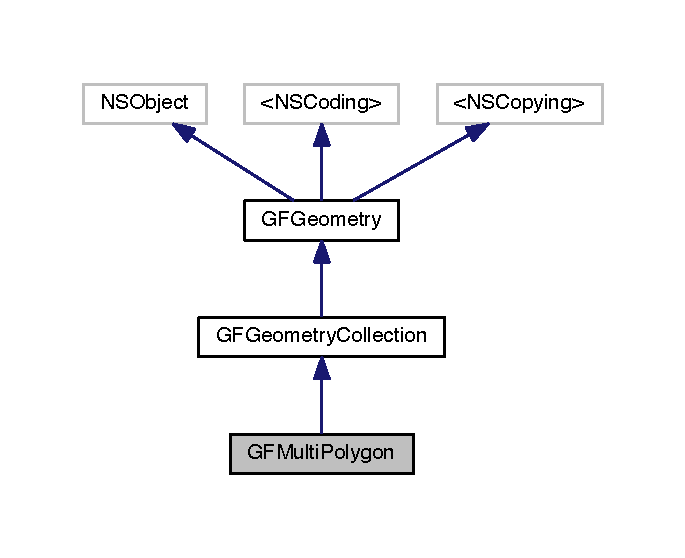
\includegraphics[width=350pt]{interface_g_f_multi_polygon__inherit__graph}
\end{center}
\end{figure}


Collaboration diagram for G\+F\+Multi\+Polygon\+:\nopagebreak
\begin{figure}[H]
\begin{center}
\leavevmode
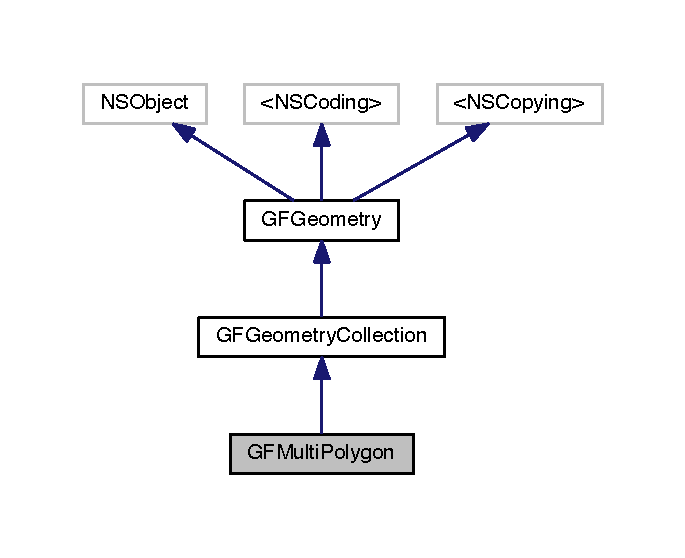
\includegraphics[width=350pt]{interface_g_f_multi_polygon__coll__graph}
\end{center}
\end{figure}
\subsection*{Instance Methods}
\begin{DoxyCompactItemize}
\item 
(instancetype) -\/ \hyperlink{interface_g_f_multi_polygon_a321e0b2c64e6dbe079205f1c58a17a2f}{init\+With\+W\+K\+T\+:}
\item 
(instancetype) -\/ \hyperlink{interface_g_f_multi_polygon_a719e2a53a9fa5e29735d53f8fc9d9071}{init\+With\+W\+K\+T\+:error\+:}
\item 
(instancetype) -\/ \hyperlink{interface_g_f_multi_polygon_a2c8f29141e272aad174a9f65190d7cab}{init\+With\+Geo\+J\+S\+O\+N\+Geometry\+:}
\item 
(instancetype) -\/ \hyperlink{interface_g_f_multi_polygon_acc419d7ae28145fa7d47186b9d125e98}{init\+With\+Geo\+J\+S\+O\+N\+Geometry\+:error\+:}
\item 
(N\+S\+U\+Integer) -\/ \hyperlink{interface_g_f_multi_polygon_a268a15cb86f1a8a57bb9f7c7f07b6443}{count}
\item 
(\hyperlink{interface_g_f_polygon}{G\+F\+Polygon} $\ast$) -\/ \hyperlink{interface_g_f_multi_polygon_ab18a262a8d02f4b15250bad1d8073f2a}{geometry\+At\+Index\+:}
\item 
(\hyperlink{interface_g_f_polygon}{G\+F\+Polygon} $\ast$) -\/ \hyperlink{interface_g_f_multi_polygon_a7dca748ca40ba2e1de638d4aaf251144}{first\+Geometry}
\item 
(\hyperlink{interface_g_f_polygon}{G\+F\+Polygon} $\ast$) -\/ \hyperlink{interface_g_f_multi_polygon_a8aa2546c3a714b390a5d2580d1356b62}{last\+Geometry}
\item 
(\hyperlink{interface_g_f_polygon}{G\+F\+Polygon} $\ast$) -\/ \hyperlink{interface_g_f_multi_polygon_ac0de2e4160cbb5e83522fc72502f681c}{object\+At\+Indexed\+Subscript\+:}
\end{DoxyCompactItemize}
\subsection*{Additional Inherited Members}


\subsection{Detailed Description}
A collection of G\+F\+Polygons. 

\begin{DoxyAuthor}{Author}
Tony Stone 
\end{DoxyAuthor}
\begin{DoxyDate}{Date}
6/14/15 
\end{DoxyDate}


\subsection{Method Documentation}
\hypertarget{interface_g_f_multi_polygon_a321e0b2c64e6dbe079205f1c58a17a2f}{}\index{G\+F\+Multi\+Polygon@{G\+F\+Multi\+Polygon}!init\+With\+W\+K\+T\+:@{init\+With\+W\+K\+T\+:}}
\index{init\+With\+W\+K\+T\+:@{init\+With\+W\+K\+T\+:}!G\+F\+Multi\+Polygon@{G\+F\+Multi\+Polygon}}
\subsubsection[{init\+With\+W\+K\+T\+:(\+N\+S\+String $\ast$wkt)}]{\setlength{\rightskip}{0pt plus 5cm}-\/ (instancetype) init\+With\+W\+K\+T\+: 
\begin{DoxyParamCaption}
\item[{(N\+S\+String $\ast$)}]{wkt}
\end{DoxyParamCaption}
}\label{interface_g_f_multi_polygon_a321e0b2c64e6dbe079205f1c58a17a2f}
Initialize this geometry with the given W\+K\+T (Well-\/\+Known-\/\+Text) string.

Example\+: 
\begin{DoxyCode}
\{

  NSString * wkt = \textcolor{stringliteral}{@"MULTIPOLYGON(((20 0,20 10,40 10,40 0,20 0)),((5 5,5 8,8 8,8 5,5 5)))"};

  \hyperlink{interface_g_f_multi_polygon}{GFMultiPolygon} * multiPolygon = [[\hyperlink{interface_g_f_multi_polygon}{GFMultiPolygon} alloc] initWithWKT: wkt]];

\}
\end{DoxyCode}
 

Reimplemented from \hyperlink{interface_g_f_geometry_collection_a13156620e5298fe7d286bb800df4097b}{G\+F\+Geometry\+Collection}.

\hypertarget{interface_g_f_multi_polygon_a719e2a53a9fa5e29735d53f8fc9d9071}{}\index{G\+F\+Multi\+Polygon@{G\+F\+Multi\+Polygon}!init\+With\+W\+K\+T\+:error\+:@{init\+With\+W\+K\+T\+:error\+:}}
\index{init\+With\+W\+K\+T\+:error\+:@{init\+With\+W\+K\+T\+:error\+:}!G\+F\+Multi\+Polygon@{G\+F\+Multi\+Polygon}}
\subsubsection[{init\+With\+W\+K\+T\+:error\+:(\+N\+S\+String $\ast$wkt,[error] N\+S\+Error $\ast$\+\_\+\+\_\+autoreleasing $\ast$\+\_\+\+Nullable error)}]{\setlength{\rightskip}{0pt plus 5cm}-\/ (instancetype) {\bf init\+With\+W\+K\+T\+:} 
\begin{DoxyParamCaption}
\item[{(N\+S\+String $\ast$)}]{wkt}
\item[{error:(N\+S\+Error $\ast$\+\_\+\+\_\+autoreleasing $\ast$\+\_\+\+Nullable)}]{error}
\end{DoxyParamCaption}
}\label{interface_g_f_multi_polygon_a719e2a53a9fa5e29735d53f8fc9d9071}
Initialize this geometry with the given W\+K\+T (Well-\/\+Known-\/\+Text) string.

Example\+: 
\begin{DoxyCode}
\{

  NSString * wkt = \textcolor{stringliteral}{@"MULTIPOLYGON(((20 0,20 10,40 10,40 0,20 0)),((5 5,5 8,8 8,8 5,5 5)))"};

  NSError * error = nil;

  \hyperlink{interface_g_f_multi_polygon}{GFMultiPolygon} * multiPolygon = [[\hyperlink{interface_g_f_multi_polygon}{GFMultiPolygon} alloc] initWithWKT: wkt 
      error: &error]];

\}
\end{DoxyCode}
 

Reimplemented from \hyperlink{interface_g_f_geometry_collection_a7569568bacbb3b0f73c60369a0dc710e}{G\+F\+Geometry\+Collection}.

\hypertarget{interface_g_f_multi_polygon_a2c8f29141e272aad174a9f65190d7cab}{}\index{G\+F\+Multi\+Polygon@{G\+F\+Multi\+Polygon}!init\+With\+Geo\+J\+S\+O\+N\+Geometry\+:@{init\+With\+Geo\+J\+S\+O\+N\+Geometry\+:}}
\index{init\+With\+Geo\+J\+S\+O\+N\+Geometry\+:@{init\+With\+Geo\+J\+S\+O\+N\+Geometry\+:}!G\+F\+Multi\+Polygon@{G\+F\+Multi\+Polygon}}
\subsubsection[{init\+With\+Geo\+J\+S\+O\+N\+Geometry\+:(\+N\+S\+Dictionary $\ast$json\+Dictionary)}]{\setlength{\rightskip}{0pt plus 5cm}-\/ (instancetype) init\+With\+Geo\+J\+S\+O\+N\+Geometry\+: 
\begin{DoxyParamCaption}
\item[{(N\+S\+Dictionary $\ast$)}]{json\+Dictionary}
\end{DoxyParamCaption}
}\label{interface_g_f_multi_polygon_a2c8f29141e272aad174a9f65190d7cab}
Initialize this geometry with the given json\+Dictionary.

\begin{DoxyNote}{Note}


You must pass the geometry portion of the Geo\+J\+S\+O\+N structure and not the entire Geo\+J\+S\+O\+N object.

Example\+:


\begin{DoxyCode}
\{
      \textcolor{stringliteral}{"type"}: \textcolor{stringliteral}{"Feature"},

      \textcolor{stringliteral}{"geometry"}: \{
                      \textcolor{stringliteral}{"type"}: \textcolor{stringliteral}{"MultiPolygon"},
                      \textcolor{stringliteral}{"coordinates"}: [
                           [
                              [[102.0, 2.0], [103.0, 2.0], [103.0, 3.0], [102.0, 3.0], [102.0, 2.0]]
                           ],
                           [
                              [[100.0, 0.0], [101.0, 0.0], [101.0, 1.0], [100.0, 1.0], [100.0, 0.0]],
                              [[100.2, 0.2], [100.8, 0.2], [100.8, 0.8], [100.2, 0.8], [100.2, 0.2]]
                           ]
                      ]
                  \}
 \}
\end{DoxyCode}


In the above example only the dictionary below that represents the geometry portion is passed.


\begin{DoxyCode}
 \{
     \textcolor{stringliteral}{"type"}: \textcolor{stringliteral}{"MultiPolygon"},
     \textcolor{stringliteral}{"coordinates"}: [
          [
            [[102.0, 2.0], [103.0, 2.0], [103.0, 3.0], [102.0, 3.0], [102.0, 2.0]]
          ],
          [
            [[100.0, 0.0], [101.0, 0.0], [101.0, 1.0], [100.0, 1.0], [100.0, 0.0]],
            [[100.2, 0.2], [100.8, 0.2], [100.8, 0.8], [100.2, 0.8], [100.2, 0.2]]
          ]
       ]
\}
\end{DoxyCode}
 
\end{DoxyNote}


Reimplemented from \hyperlink{interface_g_f_geometry_collection_adc8a317a694f82808d1e02e53e300f8f}{G\+F\+Geometry\+Collection}.

\hypertarget{interface_g_f_multi_polygon_acc419d7ae28145fa7d47186b9d125e98}{}\index{G\+F\+Multi\+Polygon@{G\+F\+Multi\+Polygon}!init\+With\+Geo\+J\+S\+O\+N\+Geometry\+:error\+:@{init\+With\+Geo\+J\+S\+O\+N\+Geometry\+:error\+:}}
\index{init\+With\+Geo\+J\+S\+O\+N\+Geometry\+:error\+:@{init\+With\+Geo\+J\+S\+O\+N\+Geometry\+:error\+:}!G\+F\+Multi\+Polygon@{G\+F\+Multi\+Polygon}}
\subsubsection[{init\+With\+Geo\+J\+S\+O\+N\+Geometry\+:error\+:(\+N\+S\+Dictionary $\ast$json\+Dictionary,[error] N\+S\+Error $\ast$\+\_\+\+\_\+autoreleasing $\ast$error)}]{\setlength{\rightskip}{0pt plus 5cm}-\/ (instancetype) {\bf init\+With\+Geo\+J\+S\+O\+N\+Geometry\+:} 
\begin{DoxyParamCaption}
\item[{(N\+S\+Dictionary $\ast$)}]{json\+Dictionary}
\item[{error:(N\+S\+Error $\ast$\+\_\+\+\_\+autoreleasing $\ast$)}]{error}
\end{DoxyParamCaption}
}\label{interface_g_f_multi_polygon_acc419d7ae28145fa7d47186b9d125e98}
Initialize this geometry with the given json\+Dictionary.

\begin{DoxyNote}{Note}


You must pass the geometry portion of the Geo\+J\+S\+O\+N structure and not the entire Geo\+J\+S\+O\+N object.

Example\+:


\begin{DoxyCode}
\{
      \textcolor{stringliteral}{"type"}: \textcolor{stringliteral}{"Feature"},

      \textcolor{stringliteral}{"geometry"}: \{
                      \textcolor{stringliteral}{"type"}: \textcolor{stringliteral}{"MultiPolygon"},
                      \textcolor{stringliteral}{"coordinates"}: [
                           [
                              [[102.0, 2.0], [103.0, 2.0], [103.0, 3.0], [102.0, 3.0], [102.0, 2.0]]
                           ],
                           [
                              [[100.0, 0.0], [101.0, 0.0], [101.0, 1.0], [100.0, 1.0], [100.0, 0.0]],
                              [[100.2, 0.2], [100.8, 0.2], [100.8, 0.8], [100.2, 0.8], [100.2, 0.2]]
                           ]
                      ]
                  \}
 \}
\end{DoxyCode}


In the above example only the dictionary below that represents the geometry portion is passed.


\begin{DoxyCode}
 \{
     \textcolor{stringliteral}{"type"}: \textcolor{stringliteral}{"MultiPolygon"},
     \textcolor{stringliteral}{"coordinates"}: [
          [
            [[102.0, 2.0], [103.0, 2.0], [103.0, 3.0], [102.0, 3.0], [102.0, 2.0]]
          ],
          [
            [[100.0, 0.0], [101.0, 0.0], [101.0, 1.0], [100.0, 1.0], [100.0, 0.0]],
            [[100.2, 0.2], [100.8, 0.2], [100.8, 0.8], [100.2, 0.8], [100.2, 0.2]]
          ]
       ]
\}
\end{DoxyCode}
 
\end{DoxyNote}


Reimplemented from \hyperlink{interface_g_f_geometry_collection_a74b596f60b3363bb9f06b06847cb086d}{G\+F\+Geometry\+Collection}.

\hypertarget{interface_g_f_multi_polygon_a268a15cb86f1a8a57bb9f7c7f07b6443}{}\index{G\+F\+Multi\+Polygon@{G\+F\+Multi\+Polygon}!count@{count}}
\index{count@{count}!G\+F\+Multi\+Polygon@{G\+F\+Multi\+Polygon}}
\subsubsection[{count()}]{\setlength{\rightskip}{0pt plus 5cm}-\/ (N\+S\+U\+Integer) count 
\begin{DoxyParamCaption}
{}
\end{DoxyParamCaption}
}\label{interface_g_f_multi_polygon_a268a15cb86f1a8a57bb9f7c7f07b6443}
The number of \hyperlink{interface_g_f_polygon}{G\+F\+Polygon} instances in this collection.

\begin{DoxyReturn}{Returns}
The count of G\+D\+Geometry instances this collection contains.
\end{DoxyReturn}
\begin{DoxySince}{Since}
1.\+1.\+0 
\end{DoxySince}


Reimplemented from \hyperlink{interface_g_f_geometry_collection_a020dd5245b572a391ccbd1ea92699240}{G\+F\+Geometry\+Collection}.

\hypertarget{interface_g_f_multi_polygon_ab18a262a8d02f4b15250bad1d8073f2a}{}\index{G\+F\+Multi\+Polygon@{G\+F\+Multi\+Polygon}!geometry\+At\+Index\+:@{geometry\+At\+Index\+:}}
\index{geometry\+At\+Index\+:@{geometry\+At\+Index\+:}!G\+F\+Multi\+Polygon@{G\+F\+Multi\+Polygon}}
\subsubsection[{geometry\+At\+Index\+:(\+N\+S\+U\+Integer index)}]{\setlength{\rightskip}{0pt plus 5cm}-\/ ({\bf G\+F\+Polygon} $\ast$) geometry\+At\+Index\+: 
\begin{DoxyParamCaption}
\item[{(N\+S\+U\+Integer)}]{index}
\end{DoxyParamCaption}
}\label{interface_g_f_multi_polygon_ab18a262a8d02f4b15250bad1d8073f2a}
Returns the \hyperlink{interface_g_f_polygon}{G\+F\+Polygon} located at the specified index.


\begin{DoxyParams}{Parameters}
{\em index} & -\/ An index within the bounds of the collection.\\
\hline
\end{DoxyParams}
\begin{DoxyReturn}{Returns}
The \hyperlink{interface_g_f_polygon}{G\+F\+Polygon} located at index.
\end{DoxyReturn}

\begin{DoxyExceptions}{Exceptions}
{\em N\+S\+Exception,N\+S\+Range\+Exception} & If index is beyond the end of the collection (that is, if index is greater than or equal to the value returned by count), an N\+S\+Range\+Exception is raised.\\
\hline
\end{DoxyExceptions}
\begin{DoxySince}{Since}
1.\+1.\+0 
\end{DoxySince}


Reimplemented from \hyperlink{interface_g_f_geometry_collection_a4cd182279facec2850b47634aa0f6297}{G\+F\+Geometry\+Collection}.

\hypertarget{interface_g_f_multi_polygon_a7dca748ca40ba2e1de638d4aaf251144}{}\index{G\+F\+Multi\+Polygon@{G\+F\+Multi\+Polygon}!first\+Geometry@{first\+Geometry}}
\index{first\+Geometry@{first\+Geometry}!G\+F\+Multi\+Polygon@{G\+F\+Multi\+Polygon}}
\subsubsection[{first\+Geometry()}]{\setlength{\rightskip}{0pt plus 5cm}-\/ ({\bf G\+F\+Polygon} $\ast$) first\+Geometry 
\begin{DoxyParamCaption}
{}
\end{DoxyParamCaption}
}\label{interface_g_f_multi_polygon_a7dca748ca40ba2e1de638d4aaf251144}
The first \hyperlink{interface_g_f_polygon}{G\+F\+Polygon} in this collection.

\begin{DoxyReturn}{Returns}
The first \hyperlink{interface_g_f_polygon}{G\+F\+Polygon} instances contained in this collection or nil if the container is empty.
\end{DoxyReturn}
\begin{DoxySince}{Since}
1.\+1.\+0 
\end{DoxySince}


Reimplemented from \hyperlink{interface_g_f_geometry_collection_a610f72a22d76a3ce6c9eaeb2dad35c0e}{G\+F\+Geometry\+Collection}.

\hypertarget{interface_g_f_multi_polygon_a8aa2546c3a714b390a5d2580d1356b62}{}\index{G\+F\+Multi\+Polygon@{G\+F\+Multi\+Polygon}!last\+Geometry@{last\+Geometry}}
\index{last\+Geometry@{last\+Geometry}!G\+F\+Multi\+Polygon@{G\+F\+Multi\+Polygon}}
\subsubsection[{last\+Geometry()}]{\setlength{\rightskip}{0pt plus 5cm}-\/ ({\bf G\+F\+Polygon} $\ast$) last\+Geometry 
\begin{DoxyParamCaption}
{}
\end{DoxyParamCaption}
}\label{interface_g_f_multi_polygon_a8aa2546c3a714b390a5d2580d1356b62}
The last \hyperlink{interface_g_f_polygon}{G\+F\+Polygon} in this collection.

\begin{DoxyReturn}{Returns}
The last \hyperlink{interface_g_f_polygon}{G\+F\+Polygon} instances contained in this collection or nil if the container is empty.
\end{DoxyReturn}
\begin{DoxySince}{Since}
1.\+1.\+0 
\end{DoxySince}


Reimplemented from \hyperlink{interface_g_f_geometry_collection_a89b3b6e2097cf5899a6d635ddcb95ef3}{G\+F\+Geometry\+Collection}.

\hypertarget{interface_g_f_multi_polygon_ac0de2e4160cbb5e83522fc72502f681c}{}\index{G\+F\+Multi\+Polygon@{G\+F\+Multi\+Polygon}!object\+At\+Indexed\+Subscript\+:@{object\+At\+Indexed\+Subscript\+:}}
\index{object\+At\+Indexed\+Subscript\+:@{object\+At\+Indexed\+Subscript\+:}!G\+F\+Multi\+Polygon@{G\+F\+Multi\+Polygon}}
\subsubsection[{object\+At\+Indexed\+Subscript\+:(\+N\+S\+U\+Integer index)}]{\setlength{\rightskip}{0pt plus 5cm}-\/ ({\bf G\+F\+Polygon} $\ast$) object\+At\+Indexed\+Subscript\+: 
\begin{DoxyParamCaption}
\item[{(N\+S\+U\+Integer)}]{index}
\end{DoxyParamCaption}
}\label{interface_g_f_multi_polygon_ac0de2e4160cbb5e83522fc72502f681c}
Returns the \hyperlink{interface_g_f_polygon}{G\+F\+Polygon} at the specified index.


\begin{DoxyParams}{Parameters}
{\em index} & An index within the bounds of the collection.\\
\hline
\end{DoxyParams}
\begin{DoxyReturn}{Returns}
The \hyperlink{interface_g_f_polygon}{G\+F\+Polygon} located at index.
\end{DoxyReturn}
Example\+:


\begin{DoxyCode}
\{
   \hyperlink{interface_g_f_multi_polygon}{GFMultiPolygon} * multiPolygon = [[\hyperlink{interface_g_f_multi_polygon}{GFMultiPolygon} alloc] initWithWKT: \textcolor{stringliteral}{@"
      MULTIPOLYGON(((20 0,20 10,40 10,40 0,20 0)),((5 5,5 8,8 8,8 5,5 5)))"}];

   \hyperlink{interface_g_f_polygon}{GFPolygon} * polygon = multiPolygon[1];
\}
\end{DoxyCode}



\begin{DoxyExceptions}{Exceptions}
{\em N\+S\+Exception} & If index is beyond the end of the collection (that is, if index is greater than or equal to the value returned by count), an N\+S\+Range\+Exception is raised.\\
\hline
\end{DoxyExceptions}
\begin{DoxySince}{Since}
1.\+1.\+0 
\end{DoxySince}


Reimplemented from \hyperlink{interface_g_f_geometry_collection_ac67dd4526580a8a38408e39c489a7503}{G\+F\+Geometry\+Collection}.



The documentation for this class was generated from the following file\+:\begin{DoxyCompactItemize}
\item 
Geo\+Features/G\+F\+Multi\+Polygon.\+h\end{DoxyCompactItemize}

\hypertarget{interface_g_f_point}{}\section{G\+F\+Point Class Reference}
\label{interface_g_f_point}\index{G\+F\+Point@{G\+F\+Point}}


Inheritance diagram for G\+F\+Point\+:\nopagebreak
\begin{figure}[H]
\begin{center}
\leavevmode
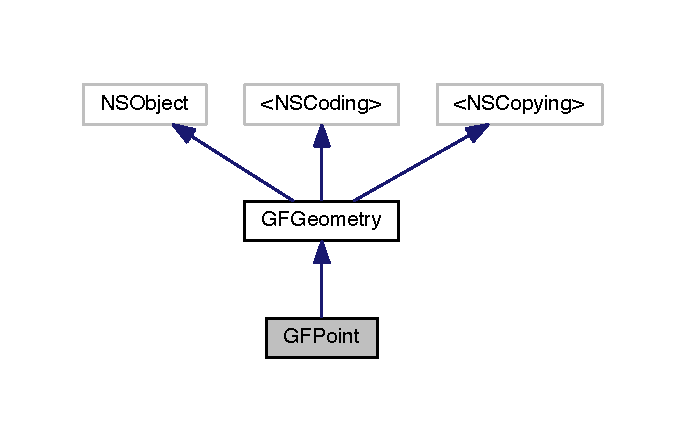
\includegraphics[width=329pt]{interface_g_f_point__inherit__graph}
\end{center}
\end{figure}


Collaboration diagram for G\+F\+Point\+:\nopagebreak
\begin{figure}[H]
\begin{center}
\leavevmode
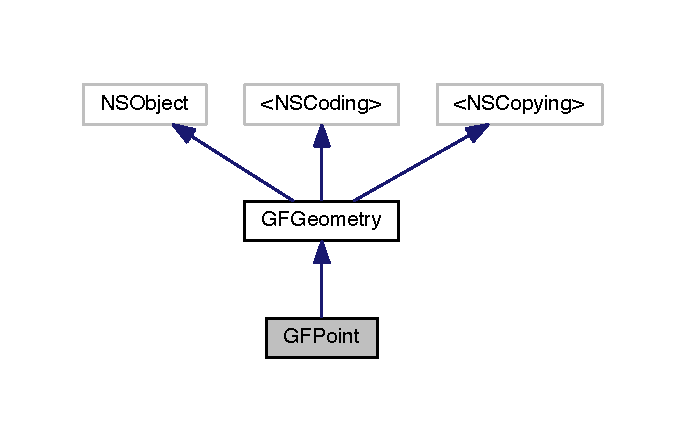
\includegraphics[width=329pt]{interface_g_f_point__coll__graph}
\end{center}
\end{figure}
\subsection*{Instance Methods}
\begin{DoxyCompactItemize}
\item 
(id) -\/ \hyperlink{interface_g_f_point_a430d98d14d3654c76f4682f53fbacf26}{init\+With\+X\+:y\+:}
\item 
(id) -\/ \hyperlink{interface_g_f_point_a85ea5cc1bf88733d818798664b991400}{init\+With\+W\+K\+T\+:}
\item 
(id) -\/ \hyperlink{interface_g_f_point_ac653a5e1489a2318bf2f00e5d7d0c03b}{init\+With\+Geo\+J\+S\+O\+N\+Geometry\+:}
\item 
(double) -\/ \hyperlink{interface_g_f_point_a5b9383f1c429724b6d938a64d468f63a}{x}
\item 
(double) -\/ \hyperlink{interface_g_f_point_a6e8ac1c0393e802c7fa7d623e0cc9599}{y}
\end{DoxyCompactItemize}
\subsection*{Additional Inherited Members}


\subsection{Method Documentation}
\hypertarget{interface_g_f_point_a430d98d14d3654c76f4682f53fbacf26}{}\index{G\+F\+Point@{G\+F\+Point}!init\+With\+X\+:y\+:@{init\+With\+X\+:y\+:}}
\index{init\+With\+X\+:y\+:@{init\+With\+X\+:y\+:}!G\+F\+Point@{G\+F\+Point}}
\subsubsection[{init\+With\+X\+:y\+:(double x,[y] double y)}]{\setlength{\rightskip}{0pt plus 5cm}-\/ (id) init\+With\+X\+: 
\begin{DoxyParamCaption}
\item[{(double)}]{x}
\item[{y:(double)}]{y}
\end{DoxyParamCaption}
}\label{interface_g_f_point_a430d98d14d3654c76f4682f53fbacf26}
Initialize this \hyperlink{interface_g_f_point}{G\+F\+Point} with the x,y coordinates \hypertarget{interface_g_f_point_a85ea5cc1bf88733d818798664b991400}{}\index{G\+F\+Point@{G\+F\+Point}!init\+With\+W\+K\+T\+:@{init\+With\+W\+K\+T\+:}}
\index{init\+With\+W\+K\+T\+:@{init\+With\+W\+K\+T\+:}!G\+F\+Point@{G\+F\+Point}}
\subsubsection[{init\+With\+W\+K\+T\+:(\+N\+S\+String $\ast$wkt)}]{\setlength{\rightskip}{0pt plus 5cm}-\/ (id) init\+With\+W\+K\+T\+: 
\begin{DoxyParamCaption}
\item[{(N\+S\+String $\ast$)}]{wkt}
\end{DoxyParamCaption}
}\label{interface_g_f_point_a85ea5cc1bf88733d818798664b991400}
Initialize this geometry with the given W\+K\+T (Well-\/\+Known-\/\+Text) string.

Example\+: 
\begin{DoxyCode}
\{

  NSString * wkt = \textcolor{stringliteral}{@"POINT(1 1)"};

  \hyperlink{interface_g_f_point}{GFPoint} * point = [[\hyperlink{interface_g_f_point}{GFPoint} alloc] initWithWKT: wkt]];

\}
\end{DoxyCode}
 \hypertarget{interface_g_f_point_ac653a5e1489a2318bf2f00e5d7d0c03b}{}\index{G\+F\+Point@{G\+F\+Point}!init\+With\+Geo\+J\+S\+O\+N\+Geometry\+:@{init\+With\+Geo\+J\+S\+O\+N\+Geometry\+:}}
\index{init\+With\+Geo\+J\+S\+O\+N\+Geometry\+:@{init\+With\+Geo\+J\+S\+O\+N\+Geometry\+:}!G\+F\+Point@{G\+F\+Point}}
\subsubsection[{init\+With\+Geo\+J\+S\+O\+N\+Geometry\+:(\+N\+S\+Dictionary $\ast$json\+Dictionary)}]{\setlength{\rightskip}{0pt plus 5cm}-\/ (id) init\+With\+Geo\+J\+S\+O\+N\+Geometry\+: 
\begin{DoxyParamCaption}
\item[{(N\+S\+Dictionary $\ast$)}]{json\+Dictionary}
\end{DoxyParamCaption}
}\label{interface_g_f_point_ac653a5e1489a2318bf2f00e5d7d0c03b}
Initialize this geometry with the given json\+Dictionary.

\begin{DoxyNote}{Note}


You must pass the geometry portion of the Geo\+J\+S\+O\+N structure and not the entire Geo\+J\+S\+O\+N object.

Example\+:


\begin{DoxyCode}
\{
      \textcolor{stringliteral}{"type"}: \textcolor{stringliteral}{"Feature"},

      \textcolor{stringliteral}{"geometry"}: \{ \textcolor{stringliteral}{"type"}: \textcolor{stringliteral}{"Point"},
                    \textcolor{stringliteral}{"coordinates"}: [100.0, 0.0]
                  \}
 \}
\end{DoxyCode}


In the above example only the dictionary below that represents the geometry portion is passed.


\begin{DoxyCode}
\{
    \textcolor{stringliteral}{"type"}: \textcolor{stringliteral}{"Point"},
    \textcolor{stringliteral}{"coordinates"}: [100.0, 0.0]
\}
\end{DoxyCode}
  
\end{DoxyNote}
\hypertarget{interface_g_f_point_a5b9383f1c429724b6d938a64d468f63a}{}\index{G\+F\+Point@{G\+F\+Point}!x@{x}}
\index{x@{x}!G\+F\+Point@{G\+F\+Point}}
\subsubsection[{x()}]{\setlength{\rightskip}{0pt plus 5cm}-\/ (double) x 
\begin{DoxyParamCaption}
{}
\end{DoxyParamCaption}
}\label{interface_g_f_point_a5b9383f1c429724b6d938a64d468f63a}
Get the point\textquotesingle{}s X value. \hypertarget{interface_g_f_point_a6e8ac1c0393e802c7fa7d623e0cc9599}{}\index{G\+F\+Point@{G\+F\+Point}!y@{y}}
\index{y@{y}!G\+F\+Point@{G\+F\+Point}}
\subsubsection[{y()}]{\setlength{\rightskip}{0pt plus 5cm}-\/ (double) y 
\begin{DoxyParamCaption}
{}
\end{DoxyParamCaption}
}\label{interface_g_f_point_a6e8ac1c0393e802c7fa7d623e0cc9599}
Get the point\textquotesingle{}s Y value. 

The documentation for this class was generated from the following file\+:\begin{DoxyCompactItemize}
\item 
G\+F\+Point.\+h\end{DoxyCompactItemize}

\hypertarget{interface_g_f_point_abstract}{}\section{G\+F\+Point\+Abstract Class Reference}
\label{interface_g_f_point_abstract}\index{G\+F\+Point\+Abstract@{G\+F\+Point\+Abstract}}


An Abstract Point implementation.  




{\ttfamily \#import $<$Geo\+Features/\+G\+F\+Point\+Abstract.\+h$>$}



Inheritance diagram for G\+F\+Point\+Abstract\+:
\nopagebreak
\begin{figure}[H]
\begin{center}
\leavevmode
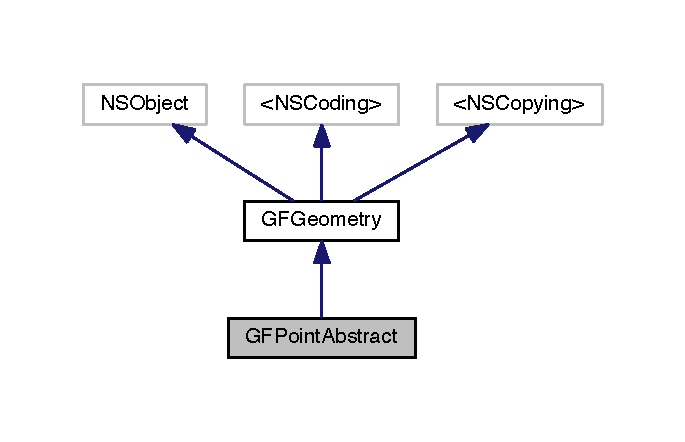
\includegraphics[width=329pt]{interface_g_f_point_abstract__inherit__graph}
\end{center}
\end{figure}


Collaboration diagram for G\+F\+Point\+Abstract\+:\nopagebreak
\begin{figure}[H]
\begin{center}
\leavevmode
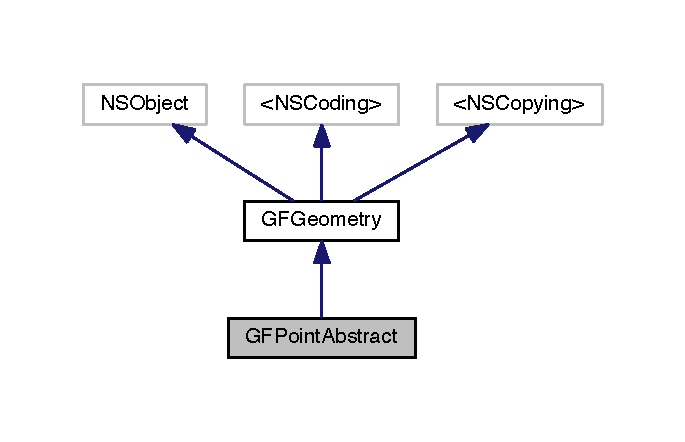
\includegraphics[width=329pt]{interface_g_f_point_abstract__coll__graph}
\end{center}
\end{figure}
\subsection*{Additional Inherited Members}


\subsection{Detailed Description}
An Abstract Point implementation. 

An Abstract Point implementation which should not be instantiated on it\textquotesingle{}s own.

\begin{DoxyWarning}{Warning}
Do not instantiate this abstract class.
\end{DoxyWarning}
\begin{DoxyAuthor}{Author}
Tony Stone 
\end{DoxyAuthor}
\begin{DoxyDate}{Date}
6/6/15 
\end{DoxyDate}


The documentation for this class was generated from the following file\+:\begin{DoxyCompactItemize}
\item 
Geo\+Features/G\+F\+Point\+Abstract.\+h\end{DoxyCompactItemize}

\hypertarget{interface_g_f_polygon}{}\section{G\+F\+Polygon Class Reference}
\label{interface_g_f_polygon}\index{G\+F\+Polygon@{G\+F\+Polygon}}


A concrete Polygon implementation.  




{\ttfamily \#import $<$Geo\+Features/\+G\+F\+Polygon.\+h$>$}



Inheritance diagram for G\+F\+Polygon\+:\nopagebreak
\begin{figure}[H]
\begin{center}
\leavevmode
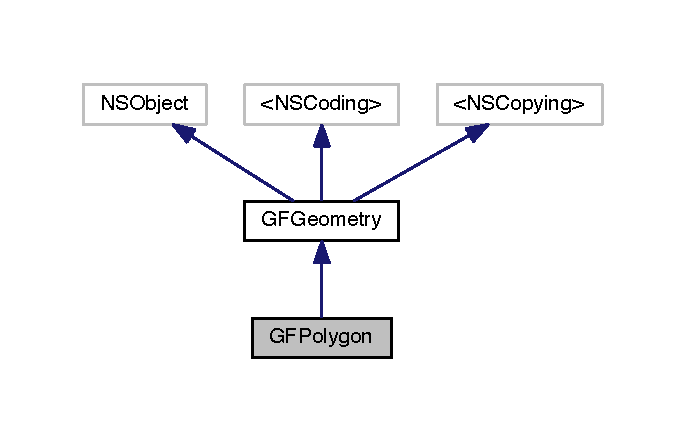
\includegraphics[width=350pt]{interface_g_f_polygon__inherit__graph}
\end{center}
\end{figure}


Collaboration diagram for G\+F\+Polygon\+:\nopagebreak
\begin{figure}[H]
\begin{center}
\leavevmode
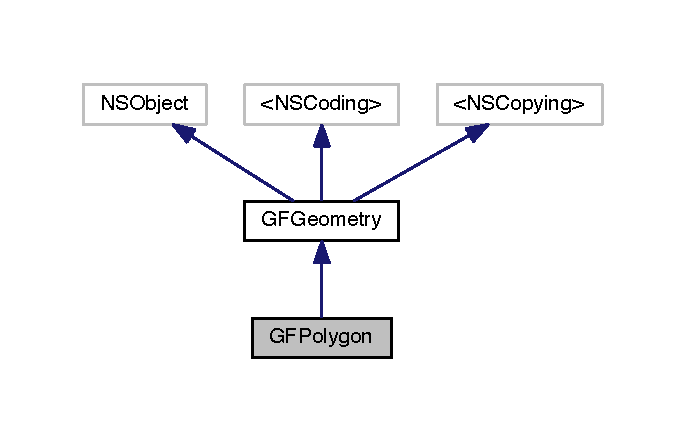
\includegraphics[width=350pt]{interface_g_f_polygon__coll__graph}
\end{center}
\end{figure}
\subsection*{Instance Methods}
\begin{DoxyCompactItemize}
\item 
(instancetype) -\/ \hyperlink{interface_g_f_polygon_a72e0e0e299103715f933177f57df2815}{init\+With\+W\+K\+T\+:}
\item 
(instancetype) -\/ \hyperlink{interface_g_f_polygon_aabc794c06956ee13f36acf6a61b2ec7c}{init\+With\+W\+K\+T\+:error\+:}
\item 
(instancetype) -\/ \hyperlink{interface_g_f_polygon_a91f132a23f38e16d5e8dea762f43ef84}{init\+With\+Geo\+J\+S\+O\+N\+Geometry\+:}
\item 
(instancetype) -\/ \hyperlink{interface_g_f_polygon_a46083a0507e17742cec90e68bc337717}{init\+With\+Geo\+J\+S\+O\+N\+Geometry\+:error\+:}
\item 
(\hyperlink{interface_g_f_ring}{G\+F\+Ring} $\ast$) -\/ \hyperlink{interface_g_f_polygon_af984fc68777e9069cd2418f6077454c1}{outer\+Ring}
\item 
(\hyperlink{interface_g_f_geometry_collection}{G\+F\+Geometry\+Collection} $\ast$) -\/ \hyperlink{interface_g_f_polygon_ae2a7ec1a59646496e5ed5e4a813909f9}{inner\+Rings}
\end{DoxyCompactItemize}
\subsection*{Additional Inherited Members}


\subsection{Detailed Description}
A concrete Polygon implementation. 

\begin{DoxyAuthor}{Author}
Tony Stone 
\end{DoxyAuthor}
\begin{DoxyDate}{Date}
6/6/15 
\end{DoxyDate}


\subsection{Method Documentation}
\hypertarget{interface_g_f_polygon_a72e0e0e299103715f933177f57df2815}{}\index{G\+F\+Polygon@{G\+F\+Polygon}!init\+With\+W\+K\+T\+:@{init\+With\+W\+K\+T\+:}}
\index{init\+With\+W\+K\+T\+:@{init\+With\+W\+K\+T\+:}!G\+F\+Polygon@{G\+F\+Polygon}}
\subsubsection[{init\+With\+W\+K\+T\+:(\+N\+S\+String $\ast$wkt)}]{\setlength{\rightskip}{0pt plus 5cm}-\/ (instancetype) init\+With\+W\+K\+T\+: 
\begin{DoxyParamCaption}
\item[{(N\+S\+String $\ast$)}]{wkt}
\end{DoxyParamCaption}
}\label{interface_g_f_polygon_a72e0e0e299103715f933177f57df2815}
Initialize this geometry with the given W\+K\+T (Well-\/\+Known-\/\+Text) string.

Example\+: 
\begin{DoxyCode}
\{

  NSString * wkt = \textcolor{stringliteral}{@"POLYGON((0 0,0 90,90 90,90 0,0 0))"};

  \hyperlink{interface_g_f_polygon}{GFPolygon} * polygon = [[\hyperlink{interface_g_f_polygon}{GFPolygon} alloc] initWithWKT: wkt]];

\}
\end{DoxyCode}
 \hypertarget{interface_g_f_polygon_aabc794c06956ee13f36acf6a61b2ec7c}{}\index{G\+F\+Polygon@{G\+F\+Polygon}!init\+With\+W\+K\+T\+:error\+:@{init\+With\+W\+K\+T\+:error\+:}}
\index{init\+With\+W\+K\+T\+:error\+:@{init\+With\+W\+K\+T\+:error\+:}!G\+F\+Polygon@{G\+F\+Polygon}}
\subsubsection[{init\+With\+W\+K\+T\+:error\+:(\+N\+S\+String $\ast$wkt,[error] N\+S\+Error $\ast$\+\_\+\+\_\+autoreleasing $\ast$error)}]{\setlength{\rightskip}{0pt plus 5cm}-\/ (instancetype) {\bf init\+With\+W\+K\+T\+:} 
\begin{DoxyParamCaption}
\item[{(N\+S\+String $\ast$)}]{wkt}
\item[{error:(N\+S\+Error $\ast$\+\_\+\+\_\+autoreleasing $\ast$)}]{error}
\end{DoxyParamCaption}
}\label{interface_g_f_polygon_aabc794c06956ee13f36acf6a61b2ec7c}
Initialize this geometry with the given W\+K\+T (Well-\/\+Known-\/\+Text) string.

Example\+: 
\begin{DoxyCode}
\{

  NSString * wkt = \textcolor{stringliteral}{@"POLYGON((0 0,0 90,90 90,90 0,0 0))"};

  NSError * error = nil;

  \hyperlink{interface_g_f_polygon}{GFPolygon} * polygon = [[\hyperlink{interface_g_f_polygon}{GFPolygon} alloc] initWithWKT: wkt error: &error]];

\}
\end{DoxyCode}
 \hypertarget{interface_g_f_polygon_a91f132a23f38e16d5e8dea762f43ef84}{}\index{G\+F\+Polygon@{G\+F\+Polygon}!init\+With\+Geo\+J\+S\+O\+N\+Geometry\+:@{init\+With\+Geo\+J\+S\+O\+N\+Geometry\+:}}
\index{init\+With\+Geo\+J\+S\+O\+N\+Geometry\+:@{init\+With\+Geo\+J\+S\+O\+N\+Geometry\+:}!G\+F\+Polygon@{G\+F\+Polygon}}
\subsubsection[{init\+With\+Geo\+J\+S\+O\+N\+Geometry\+:(\+N\+S\+Dictionary $\ast$json\+Dictionary)}]{\setlength{\rightskip}{0pt plus 5cm}-\/ (instancetype) init\+With\+Geo\+J\+S\+O\+N\+Geometry\+: 
\begin{DoxyParamCaption}
\item[{(N\+S\+Dictionary $\ast$)}]{json\+Dictionary}
\end{DoxyParamCaption}
}\label{interface_g_f_polygon_a91f132a23f38e16d5e8dea762f43ef84}
Initialize this geometry with the given json\+Dictionary.

\begin{DoxyNote}{Note}


You must pass the geometry portion of the Geo\+J\+S\+O\+N structure and not the entire Geo\+J\+S\+O\+N object.

Given the following J\+S\+O\+N\+: 
\begin{DoxyCode}
\{
      \textcolor{stringliteral}{"type"}: \textcolor{stringliteral}{"Feature"},

      \textcolor{stringliteral}{"geometry"}: \{
                      \textcolor{stringliteral}{"type"}: \textcolor{stringliteral}{"MultiPolygon"},
                      \textcolor{stringliteral}{"coordinates"}: [
                            [ [100.0, 0.0], [101.0, 0.0], [101.0, 1.0], [100.0, 1.0], [100.0, 0.0] ]
                       ]
                  \}
 \}
\end{DoxyCode}


You would pass this section to the init method. 
\begin{DoxyCode}
\{
     \textcolor{stringliteral}{"type"}: \textcolor{stringliteral}{"MultiPolygon"},
     \textcolor{stringliteral}{"coordinates"}: [
           [ [100.0, 0.0], [101.0, 0.0], [101.0, 1.0], [100.0, 1.0], [100.0, 0.0] ]
     ]
\}
\end{DoxyCode}
 
\end{DoxyNote}
\hypertarget{interface_g_f_polygon_a46083a0507e17742cec90e68bc337717}{}\index{G\+F\+Polygon@{G\+F\+Polygon}!init\+With\+Geo\+J\+S\+O\+N\+Geometry\+:error\+:@{init\+With\+Geo\+J\+S\+O\+N\+Geometry\+:error\+:}}
\index{init\+With\+Geo\+J\+S\+O\+N\+Geometry\+:error\+:@{init\+With\+Geo\+J\+S\+O\+N\+Geometry\+:error\+:}!G\+F\+Polygon@{G\+F\+Polygon}}
\subsubsection[{init\+With\+Geo\+J\+S\+O\+N\+Geometry\+:error\+:(\+N\+S\+Dictionary $\ast$json\+Dictionary,[error] N\+S\+Error $\ast$\+\_\+\+\_\+autoreleasing $\ast$error)}]{\setlength{\rightskip}{0pt plus 5cm}-\/ (instancetype) {\bf init\+With\+Geo\+J\+S\+O\+N\+Geometry\+:} 
\begin{DoxyParamCaption}
\item[{(N\+S\+Dictionary $\ast$)}]{json\+Dictionary}
\item[{error:(N\+S\+Error $\ast$\+\_\+\+\_\+autoreleasing $\ast$)}]{error}
\end{DoxyParamCaption}
}\label{interface_g_f_polygon_a46083a0507e17742cec90e68bc337717}
Initialize this geometry with the given json\+Dictionary.

\begin{DoxyNote}{Note}


You must pass the geometry portion of the Geo\+J\+S\+O\+N structure and not the entire Geo\+J\+S\+O\+N object.

Given the following J\+S\+O\+N\+: 
\begin{DoxyCode}
\{
      \textcolor{stringliteral}{"type"}: \textcolor{stringliteral}{"Feature"},

      \textcolor{stringliteral}{"geometry"}: \{
                      \textcolor{stringliteral}{"type"}: \textcolor{stringliteral}{"MultiPolygon"},
                      \textcolor{stringliteral}{"coordinates"}: [
                            [ [100.0, 0.0], [101.0, 0.0], [101.0, 1.0], [100.0, 1.0], [100.0, 0.0] ]
                       ]
                  \}
 \}
\end{DoxyCode}


You would pass this section to the init method. 
\begin{DoxyCode}
\{
     \textcolor{stringliteral}{"type"}: \textcolor{stringliteral}{"MultiPolygon"},
     \textcolor{stringliteral}{"coordinates"}: [
           [ [100.0, 0.0], [101.0, 0.0], [101.0, 1.0], [100.0, 1.0], [100.0, 0.0] ]
     ]
\}
\end{DoxyCode}
 
\end{DoxyNote}
\hypertarget{interface_g_f_polygon_af984fc68777e9069cd2418f6077454c1}{}\index{G\+F\+Polygon@{G\+F\+Polygon}!outer\+Ring@{outer\+Ring}}
\index{outer\+Ring@{outer\+Ring}!G\+F\+Polygon@{G\+F\+Polygon}}
\subsubsection[{outer\+Ring()}]{\setlength{\rightskip}{0pt plus 5cm}-\/ ({\bf G\+F\+Ring} $\ast$) outer\+Ring 
\begin{DoxyParamCaption}
{}
\end{DoxyParamCaption}
}\label{interface_g_f_polygon_af984fc68777e9069cd2418f6077454c1}
The outer ring of this polygon.

\begin{DoxyReturn}{Returns}
The outer \hyperlink{interface_g_f_ring}{G\+F\+Ring} of this polygon. 
\end{DoxyReturn}
\hypertarget{interface_g_f_polygon_ae2a7ec1a59646496e5ed5e4a813909f9}{}\index{G\+F\+Polygon@{G\+F\+Polygon}!inner\+Rings@{inner\+Rings}}
\index{inner\+Rings@{inner\+Rings}!G\+F\+Polygon@{G\+F\+Polygon}}
\subsubsection[{inner\+Rings()}]{\setlength{\rightskip}{0pt plus 5cm}-\/ ({\bf G\+F\+Geometry\+Collection} $\ast$) inner\+Rings 
\begin{DoxyParamCaption}
{}
\end{DoxyParamCaption}
}\label{interface_g_f_polygon_ae2a7ec1a59646496e5ed5e4a813909f9}
The inner rings of this polygon.

\begin{DoxyReturn}{Returns}
A collection of inner G\+F\+Rings of this polygon. 
\end{DoxyReturn}


The documentation for this class was generated from the following file\+:\begin{DoxyCompactItemize}
\item 
Geo\+Features/G\+F\+Polygon.\+h\end{DoxyCompactItemize}

\hypertarget{interface_g_f_polygon_abstract}{}\section{G\+F\+Polygon\+Abstract Class Reference}
\label{interface_g_f_polygon_abstract}\index{G\+F\+Polygon\+Abstract@{G\+F\+Polygon\+Abstract}}


An Abstract Polygon implementation.  




{\ttfamily \#import $<$Geo\+Features/\+G\+F\+Polygon\+Abstract.\+h$>$}



Inheritance diagram for G\+F\+Polygon\+Abstract\+:\nopagebreak
\begin{figure}[H]
\begin{center}
\leavevmode
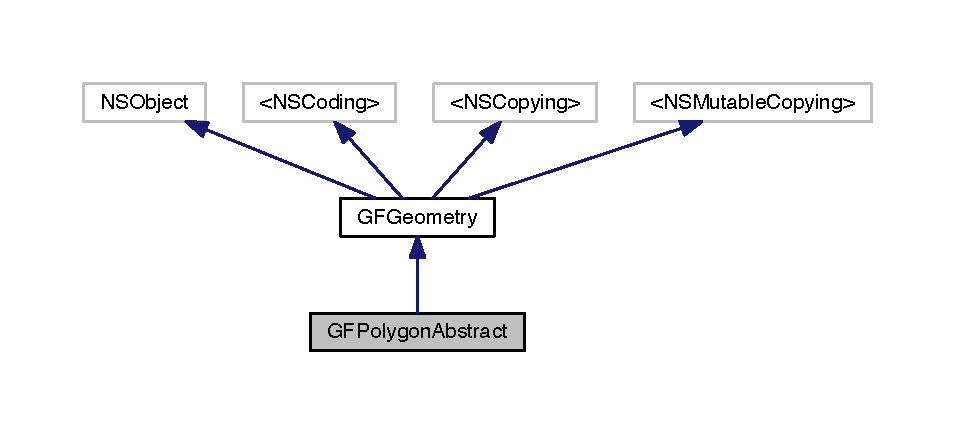
\includegraphics[width=329pt]{interface_g_f_polygon_abstract__inherit__graph}
\end{center}
\end{figure}


Collaboration diagram for G\+F\+Polygon\+Abstract\+:\nopagebreak
\begin{figure}[H]
\begin{center}
\leavevmode
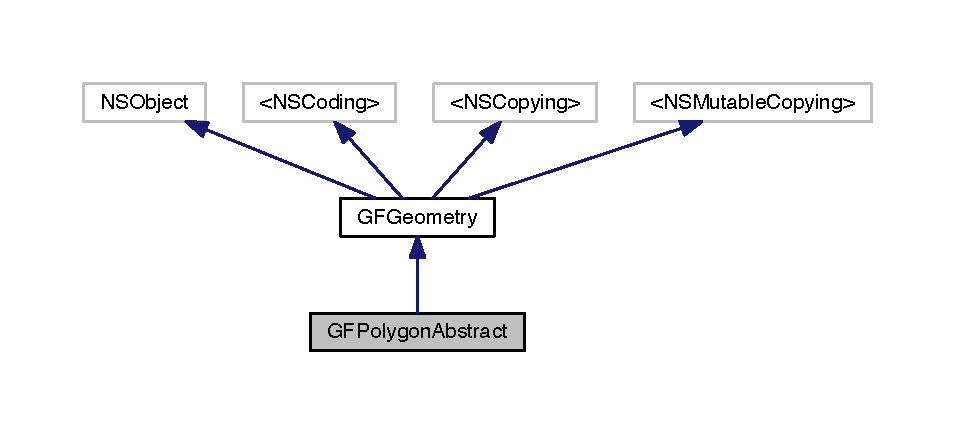
\includegraphics[width=329pt]{interface_g_f_polygon_abstract__coll__graph}
\end{center}
\end{figure}
\subsection*{Additional Inherited Members}


\subsection{Detailed Description}
An Abstract Polygon implementation. 

An Abstract Polygon implementation which should not be instantiated on it\textquotesingle{}s own.

\begin{DoxyWarning}{Warning}
Do not instantiate this abstract class.
\end{DoxyWarning}
\begin{DoxyAuthor}{Author}
Tony Stone 
\end{DoxyAuthor}
\begin{DoxyDate}{Date}
6/6/15 
\end{DoxyDate}


The documentation for this class was generated from the following file\+:\begin{DoxyCompactItemize}
\item 
Geo\+Features/G\+F\+Polygon\+Abstract.\+h\end{DoxyCompactItemize}

\hypertarget{interface_g_f_ring}{}\section{G\+F\+Ring Class Reference}
\label{interface_g_f_ring}\index{G\+F\+Ring@{G\+F\+Ring}}


A \hyperlink{interface_g_f_ring}{G\+F\+Ring} (aka linear ring) is a closed line which should not be self intersecting.  




{\ttfamily \#import $<$Geo\+Features/\+G\+F\+Ring.\+h$>$}



Inheritance diagram for G\+F\+Ring\+:\nopagebreak
\begin{figure}[H]
\begin{center}
\leavevmode
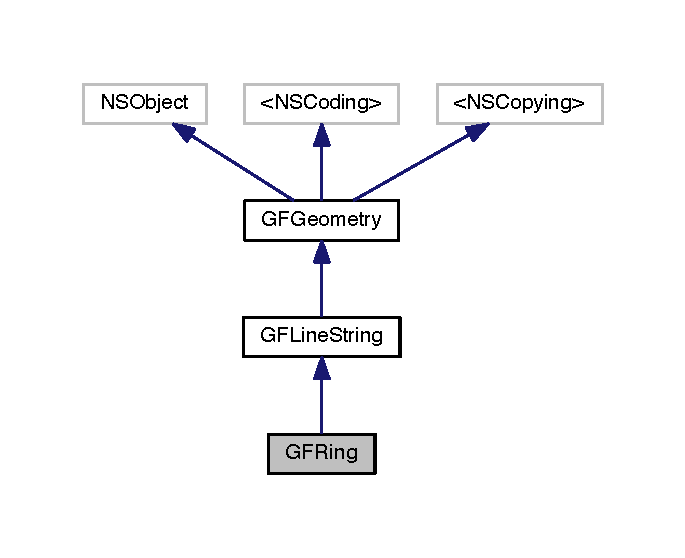
\includegraphics[width=350pt]{interface_g_f_ring__inherit__graph}
\end{center}
\end{figure}


Collaboration diagram for G\+F\+Ring\+:\nopagebreak
\begin{figure}[H]
\begin{center}
\leavevmode
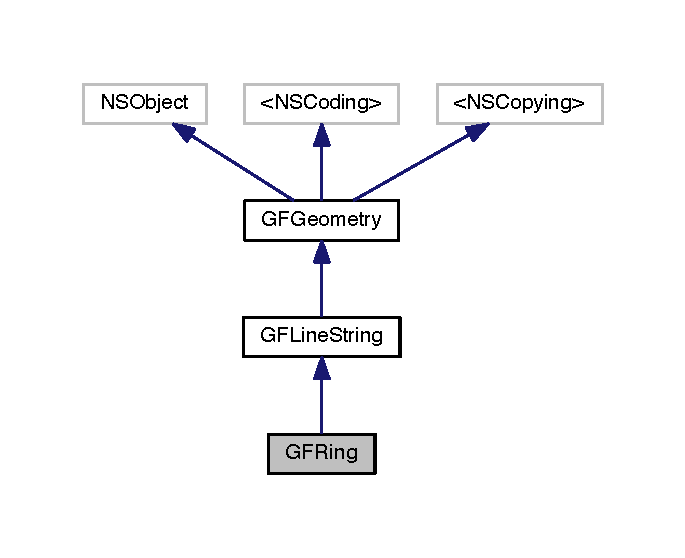
\includegraphics[width=350pt]{interface_g_f_ring__coll__graph}
\end{center}
\end{figure}
\subsection*{Instance Methods}
\begin{DoxyCompactItemize}
\item 
(instancetype) -\/ \hyperlink{interface_g_f_ring_a063be826fc24346e1fb5d4830f641ef0}{init\+With\+W\+K\+T\+:}
\item 
(instancetype) -\/ \hyperlink{interface_g_f_ring_a3562a7a5b8b37c53de97a0c31981c907}{init\+With\+Geo\+J\+S\+O\+N\+Geometry\+:}
\end{DoxyCompactItemize}
\subsection*{Additional Inherited Members}


\subsection{Detailed Description}
A \hyperlink{interface_g_f_ring}{G\+F\+Ring} (aka linear ring) is a closed line which should not be self intersecting. 

A \hyperlink{interface_g_f_ring}{G\+F\+Ring} is a \hyperlink{interface_g_f_line_string}{G\+F\+Line\+String} which is closed. The first and last coordinate in the ring must be equal, and the interior of the ring must not self-\/intersect. A ring must have either 0 or 4 or more G\+F\+Points. If these conditions are not met, the constructors throw an Illegal\+Argument\+Exception

\begin{DoxyAuthor}{Author}
Tony Stone 
\end{DoxyAuthor}
\begin{DoxyDate}{Date}
8/30/15 
\end{DoxyDate}


\subsection{Method Documentation}
\hypertarget{interface_g_f_ring_a063be826fc24346e1fb5d4830f641ef0}{}\index{G\+F\+Ring@{G\+F\+Ring}!init\+With\+W\+K\+T\+:@{init\+With\+W\+K\+T\+:}}
\index{init\+With\+W\+K\+T\+:@{init\+With\+W\+K\+T\+:}!G\+F\+Ring@{G\+F\+Ring}}
\subsubsection[{init\+With\+W\+K\+T\+:(\+N\+S\+String $\ast$wkt)}]{\setlength{\rightskip}{0pt plus 5cm}-\/ (instancetype) init\+With\+W\+K\+T\+: 
\begin{DoxyParamCaption}
\item[{(N\+S\+String $\ast$)}]{wkt}
\end{DoxyParamCaption}
}\label{interface_g_f_ring_a063be826fc24346e1fb5d4830f641ef0}
\begin{DoxySeeAlso}{See also}
\hyperlink{interface_g_f_line_string}{G\+F\+Line\+String} for methods Initialize this geometry with the given W\+K\+T (Well-\/\+Known-\/\+Text) string.
\end{DoxySeeAlso}
\begin{DoxyNote}{Note}


W\+K\+T does not support rings. However, to be generic Geo\+Features supports reading and writing from and to rings. Rings are read and written as a standard L\+I\+N\+E\+S\+T\+R\+I\+N\+G W\+K\+T.


\end{DoxyNote}


Example\+: 
\begin{DoxyCode}
\{

  NSString * wkt = \textcolor{stringliteral}{@"LINESTRING(40 60,120 110)"};

  \hyperlink{interface_g_f_ring}{GFRing} * ring = [[\hyperlink{interface_g_f_ring}{GFRing} alloc] initWithWKT: wkt]];

\}
\end{DoxyCode}
 

Reimplemented from \hyperlink{interface_g_f_line_string_a261a4d08fe5cb35f935d265c3a97f453}{G\+F\+Line\+String}.

\hypertarget{interface_g_f_ring_a3562a7a5b8b37c53de97a0c31981c907}{}\index{G\+F\+Ring@{G\+F\+Ring}!init\+With\+Geo\+J\+S\+O\+N\+Geometry\+:@{init\+With\+Geo\+J\+S\+O\+N\+Geometry\+:}}
\index{init\+With\+Geo\+J\+S\+O\+N\+Geometry\+:@{init\+With\+Geo\+J\+S\+O\+N\+Geometry\+:}!G\+F\+Ring@{G\+F\+Ring}}
\subsubsection[{init\+With\+Geo\+J\+S\+O\+N\+Geometry\+:(\+N\+S\+Dictionary $\ast$json\+Dictionary)}]{\setlength{\rightskip}{0pt plus 5cm}-\/ (instancetype) init\+With\+Geo\+J\+S\+O\+N\+Geometry\+: 
\begin{DoxyParamCaption}
\item[{(N\+S\+Dictionary $\ast$)}]{json\+Dictionary}
\end{DoxyParamCaption}
}\label{interface_g_f_ring_a3562a7a5b8b37c53de97a0c31981c907}
Initialize this geometry with the given json\+Dictionary.

\begin{DoxyNote}{Note}


Geo\+J\+S\+O\+N does not support rings. However, to be generic Geo\+Features supports reading and writing from and to rings. Rings are read and written as a standard Geo\+J\+S\+O\+N Line\+String.

You must pass the geometry portion of the Geo\+J\+S\+O\+N structure and not the entire Geo\+J\+S\+O\+N object.

Example\+:


\begin{DoxyCode}
\{
      \textcolor{stringliteral}{"type"}: \textcolor{stringliteral}{"Feature"},

      \textcolor{stringliteral}{"geometry"}: \{ \textcolor{stringliteral}{"type"}: \textcolor{stringliteral}{"LineString"},
                    \textcolor{stringliteral}{"coordinates"}: [ [100.0, 0.0], [101.0, 1.0] ]
                  \}
 \}
\end{DoxyCode}


In the above example only the dictionary below that represents the geometry portion is passed.


\begin{DoxyCode}
\{
      \textcolor{stringliteral}{"type"}: \textcolor{stringliteral}{"LineString"},
      \textcolor{stringliteral}{"coordinates"}: [ [100.0, 0.0], [101.0, 1.0] ]
\}
\end{DoxyCode}
 
\end{DoxyNote}


Reimplemented from \hyperlink{interface_g_f_line_string_ad7a913bc12b6099982229190d1debd71}{G\+F\+Line\+String}.



The documentation for this class was generated from the following file\+:\begin{DoxyCompactItemize}
\item 
Geo\+Features/G\+F\+Ring.\+h\end{DoxyCompactItemize}

%--- End generated contents ---

% Index
\backmatter
\newpage
\phantomsection
\clearemptydoublepage
\addcontentsline{toc}{chapter}{Index}
\printindex

\end{document}
